% ============================================================================
%  Final Report Template — EAFIT University
%  Optical Methods in the Atmosphere
%  Emmanuel Mazó Gómez
% ============================================================================
\documentclass[a4paper, 11pt]{article}

% --- Encoding & Language ---
\usepackage[utf8]{inputenc}
\usepackage[T1]{fontenc}
\usepackage[english]{babel}

% --- Page geometry ---
\usepackage[
  top=2cm,
  bottom=1.8cm,
  left=1.8cm,
  right=1.8cm,
  headheight=2.0cm,
  headsep=0.5cm,
  footskip=1.0cm
]{geometry}

% --- Fonts ---
\usepackage{lmodern}
\usepackage{microtype}

% --- Math ---
\usepackage{amsmath, amssymb, amsfonts, bm}

% --- Graphics & Figures ---
\usepackage{graphicx}
\usepackage{float}
\usepackage{subcaption}
\usepackage{tikz}

% --- Tables ---
\usepackage{booktabs}
\usepackage{array}
\usepackage{multirow}

% --- Colors — EAFIT Institutional Palette ---
\usepackage{xcolor}
\definecolor{eafitNavy}{HTML}{003366}      % EAFIT primary dark blue
\definecolor{eafitBlue}{HTML}{004B8D}      % EAFIT medium blue
\definecolor{eafitGold}{HTML}{D4A843}      % EAFIT gold/yellow accent
\definecolor{eafitLightGray}{HTML}{F2F2F2} % Light background
\definecolor{eafitDarkGray}{HTML}{333333}   % Text color

% --- Headers & Footers ---
\usepackage{fancyhdr}
\pagestyle{fancy}
\fancyhf{}

% Header: logo left, course info right
\lhead{%
  \raisebox{-0.3\height}{%
    
\includegraphics[height=1.2cm]{logos/eafit_logo.png}% <-- Place your logo here
  }%
}
\rhead{%
  \small\color{eafitNavy}%
  \textbf{Universidad EAFIT}\\
  \textit{Optical Methods}%
}
\renewcommand{\headrulewidth}{1.5pt}
\renewcommand{\headrule}{\hbox to\headwidth{\color{eafitNavy}\leaders\hrule height \headrulewidth\hfill}}

% Footer: page number centered
\cfoot{\thepage}
\renewcommand{\footrulewidth}{0.4pt}
\renewcommand{\footrule}{\hbox to\headwidth{\color{eafitNavy}\leaders\hrule height \footrulewidth\hfill}}

% First-page style (for title page)
\fancypagestyle{plain}{
  \fancyhf{}
  \cfoot{\thepage}
  \renewcommand{\headrulewidth}{0pt}
  \renewcommand{\footrulewidth}{0.4pt}
  \renewcommand{\footrule}{\hbox to\headwidth{\color{eafitNavy}\leaders\hrule height \footrulewidth\hfill}}
}

% --- Hyperlinks ---
\usepackage[
  colorlinks=true,
  linkcolor=eafitNavy,
  citecolor=eafitBlue,
  urlcolor=eafitBlue
]{hyperref}

% --- Section styling ---
\usepackage{titlesec}

\titleformat{\section}
  {\Large\bfseries\color{eafitNavy}}
  {\thesection}{1em}{}
  [\vspace{2pt}{\color{eafitGold}\titlerule[1.5pt]}]

\titleformat{\subsection}
  {\large\bfseries\color{eafitBlue}}
  {\thesubsection}{1em}{}

\titleformat{\subsubsection}
  {\normalsize\bfseries\color{eafitNavy}}
  {\thesubsubsection}{1em}{}

% --- Colored boxes ---
\usepackage{tcolorbox}
\tcbuselibrary{skins, breakable}

\newtcolorbox{eafitbox}[1]{
  enhanced,
  colback=eafitLightGray,
  colframe=eafitNavy,
  coltitle=white,
  fonttitle=\bfseries,
  title={#1},
  arc=2pt,
  boxrule=1pt,
  breakable
}

\newtcolorbox{resultbox}[1]{
  enhanced,
  colback=white,
  colframe=eafitGold,
  coltitle=eafitNavy,
  fonttitle=\bfseries,
  title={#1},
  arc=2pt,
  boxrule=1.2pt,
  breakable
}

% --- Code listings ---
\usepackage{listings}
\lstset{
  language=Python,
  basicstyle=\ttfamily\small,
  keywordstyle=\color{eafitNavy}\bfseries,
  commentstyle=\color{gray}\itshape,
  stringstyle=\color{eafitGold!80!black},
  backgroundcolor=\color{eafitLightGray},
  frame=single,
  rulecolor=\color{eafitNavy},
  breaklines=true,
  numbers=left,
  numberstyle=\tiny\color{gray},
  tabsize=4,
  showstringspaces=false
}

% --- Bibliography ---
\usepackage[numbers, sort&compress]{natbib}

% --- Misc ---
\usepackage{enumitem}
\setlist{noitemsep, topsep=4pt}

% ============================================================================
%                           DOCUMENT BEGINS
% ============================================================================
\begin{document}

% ~~~~~~~~~~~~~~~~~~~~~~~~~~~~~~~~~~~~~~~~~~~~~~~~~~~~~~~~~~~~~~~~~~~~~~~~~~~~
%                            TITLE PAGE
% ~~~~~~~~~~~~~~~~~~~~~~~~~~~~~~~~~~~~~~~~~~~~~~~~~~~~~~~~~~~~~~~~~~~~~~~~~~~~
\begin{titlepage}
  \begin{center}

    % --- EAFIT Logo ---
    \vspace*{0.5cm}
    
\includegraphics[width=6cm]{logos/eafit_logo.png}% <-- Place your logo file
    \vspace{1.5cm}

    % --- University info ---
    {\large\color{eafitNavy}
      \textbf{UNIVERSIDAD EAFIT}\\[0.3cm]
      Escuela de Ciencias Aplicadas e Ingeniería\\[0.1cm]
      Maestría en Física Aplicada\\[0.1cm]
    }

    \vspace{0.5cm}
    {\color{eafitGold}\rule{0.8\textwidth}{1.5pt}}
    \vspace{1.0cm}

    % --- Title ---
    {\LARGE\bfseries\color{eafitNavy}
      Retrieval of Aerosol Optical Properties\\[0.3cm]
      Using Radiative Transfer Theory:\\[0.3cm]
      A Direct--Inverse Problem Approach
    }

    \vspace{0.8cm}
    {\color{eafitGold}\rule{0.8\textwidth}{1.5pt}}
    \vspace{1.0cm}

    % --- Subtitle ---
    {\large\color{eafitDarkGray}
      Final Report\\[0.3cm]
      \textit{Optical Methods}
    }

    \vfill

    % --- Author ---
    {\large
      \textbf{Emmanuel Mazo Gómez}\\[0.3cm]
    }

    \vspace{1cm}

    % --- Date ---
    {\large\color{eafitNavy}
      Medellín, Colombia\\[0.2cm]
      \today
    }

    \vspace{0.5cm}
  \end{center}
\end{titlepage}

% ~~~~~~~~~~~~~~~~~~~~~~~~~~~~~~~~~~~~~~~~~~~~~~~~~~~~~~~~~~~~~~~~~~~~~~~~~~~~
%                         FRONT MATTER
% ~~~~~~~~~~~~~~~~~~~~~~~~~~~~~~~~~~~~~~~~~~~~~~~~~~~~~~~~~~~~~~~~~~~~~~~~~~~~
\pagenumbering{roman}

% --- Abstract ---
\begin{abstract}
\noindent
% Write your abstract here.
This report presents the development and validation of a one-dimensional
radiative transfer model based on the Discrete Ordinates method (DISORT) for
the retrieval of aerosol optical properties from atmospheric radiance
measurements. The forward model solves the radiative transfer equation in a
multi-layer plane-parallel atmosphere with Rayleigh scattering, Mie aerosol
optics, and surface reflection. Multiple inverse techniques (Levenberg--Marquardt,
Optimal Estimation) are
implemented and compared for retrieving aerosol optical depth, single-scattering
albedo, and asymmetry parameter profiles.
\end{abstract}

\newpage
\tableofcontents
\newpage
\listoffigures
\newpage

% ~~~~~~~~~~~~~~~~~~~~~~~~~~~~~~~~~~~~~~~~~~~~~~~~~~~~~~~~~~~~~~~~~~~~~~~~~~~~
%                          MAIN BODY
% ~~~~~~~~~~~~~~~~~~~~~~~~~~~~~~~~~~~~~~~~~~~~~~~~~~~~~~~~~~~~~~~~~~~~~~~~~~~~
\pagenumbering{arabic}

% ====================================================================
\section{Introduction}
\label{sec:introduction}
% ====================================================================

Atmospheric aerosols play a central role in the Earth's radiative budget, by scattering and absorbing solar radiation, they modify the planetary albedo, alter the vertical distribution of heating rates, and constitute one of the largest sources of uncertainty in current climate projections \cite{ipcc2021}.  Quantifying their optical properties is therefore essential for climate science, satellite-based remote sensing of the Earth's surface \cite{kaufman2002}, and assessment of air quality and atmospheric visibility \cite{seinfeld2016}.

The primary measurable quantities that characterise an aerosol layer are
the aerosol optical depth~(AOD), $\tau_{\text{aer}}$, which describes
the column-integrated extinction; the single-scattering
albedo~(SSA), $\omega_0$, which gives the ratio of scattering to total
extinction; and the asymmetry parameter~$g$, which quantifies the
degree of forward scattering.  These three quantities fully determine
the first-order radiative effect (the direct perturbation to the shortwave energy balance at a given wavelength) of an aerosol population, and their retrieval from radiance measurements constitutes
a classic inverse problem in atmospheric optics \cite{rodgers2000}.

Retrieving aerosol properties from top-of-atmosphere~(TOA) radiance
measurements requires two complementary components: the \emph{forward model} computes the radiation field for a prescribed atmospheric state by solving the radiative transfer equation~(RTE) and the \emph{inverse method} then adjusts the atmospheric state until the
modelled radiances match the observations within a prescribed
tolerance.  Because the relationship between aerosol parameters and
radiances is nonlinear, and because the inverse problem is generally
ill-posed \cite{hadamard1902,tikhonov1977}, both the accuracy of the
forward solver and the choice of regularisation strategy are critical
to the quality of the retrieval.

Among the various numerical techniques available for solving the
plane-parallel RTE (including adding-doubling, Monte Carlo, and
successive orders of scattering) the Discrete Ordinates
method~(DISORT) introduced by Stamnes et al.\ \cite{stamnes1988} has become a
widely adopted standard.  DISORT replaces the continuous angular
variable by a finite set of quadrature directions, thereby reducing
the integro-differential RTE to a system of coupled ordinary
differential equations that can be solved by eigenvalue decomposition.
The method is exact for a given quadrature order, handles multiple
scattering and arbitrary vertical layering, and provides both upwelling
and downwelling intensities at all atmospheric levels.

The present work develops a complete forward--inverse modelling chain
for aerosol retrieval.  The specific objectives are:
\begin{enumerate}
  \item Formulate the plane-parallel RTE and implement a multi-layer
        DISORT solver with delta-M scaling, Mie-theory aerosol
        optics, and Lambertian surface reflection.
  \item Design and compare two inverse methods (Levenberg--Marquardt
        with Tikhonov regularisation and Optimal Estimation following
        Rodgers \cite{rodgers2000}) for the joint
        retrieval of AOD, SSA, and~$g$.
  \item Validate the forward model against analytical limiting cases
        and energy conservation constraints, and assess the retrieval
        performance on both synthetic and real data from the AERONET
        network \cite{holben1998}.
\end{enumerate}

The remainder of the report is organised as follows.
Section~\ref{sec:theory} presents the theoretical framework,
comprising the derivation of the RTE, the discrete-ordinates
formulation, Mie theory, and the mathematical basis of each inverse
method.  Section~\ref{sec:methods} describes the numerical
implementation, including the atmospheric model configuration, the
eigenvalue solver with its stabilisation techniques, and the algorithmic
details of each retrieval.  Section~\ref{sec:results} presents the
validation tests and the retrieval results for idealized, multi-layer,
and real-data scenarios.
Section~\ref{sec:uncertainty} provides an uncertainty analysis,
and Section~\ref{sec:conclusions} summarises the main findings.
\\
\\

% ====================================================================
\section{Theoretical Framework}
\label{sec:theory}
% ====================================================================

% --------------------------------------------------------------------
\subsection{The Radiative Transfer Equation}
\label{sec:rte}
% --------------------------------------------------------------------

The propagation of monochromatic radiation through a scattering and
absorbing medium is governed by the radiative transfer equation.  In a
plane-parallel atmosphere, the RTE takes the form
\cite{chandrasekhar1950,thomas2002,disortreport}
%
\begin{equation}
  \mu\,\frac{dI(\tau,\mu,\phi)}{d\tau}
  = I(\tau,\mu,\phi) - S(\tau,\mu,\phi),
  \label{eq:rte}
\end{equation}
%
where $I(\tau,\mu,\phi)$ is the specific intensity
[W\,m$^{-2}$\,sr$^{-1}$] at optical depth~$\tau$, in the direction
defined by the cosine of the zenith angle $\mu = \cos\theta$ and the
azimuth angle~$\phi$; and $S$ is the source function.  The optical
depth is a dimensionless vertical coordinate defined by
$d\tau = -\sigma_{\text{ext}}\,dz$, where $\sigma_{\text{ext}}$ is the
volume extinction coefficient and $z$ is the geometric altitude, so
that $\tau$ increases from zero at the top of the atmosphere~(TOA)
to a maximum value $\tau_{\text{total}}$ at the surface.  By convention,
$\mu > 0$ denotes upwelling (ascending) radiation, while $\mu < 0$
corresponds to downwelling (descending) radiation.

The source function contains two contributions.  The first is
multiple scattering from all directions into the direction of interest:
%
\begin{equation}
  S_{\text{scat}}(\tau,\mu,\phi)
  = \frac{\omega(\tau)}{4\pi}\int_{0}^{2\pi}\!\int_{-1}^{1}
    P(\cos\Theta)\,I(\tau,\mu',\phi')\,d\mu'\,d\phi',
  \label{eq:source_scat}
\end{equation}
%
where $\omega(\tau)$ is the single-scattering albedo, defined as the
ratio of the scattering coefficient to the total extinction coefficient,
and $P(\cos\Theta)$ is the scattering phase function, which describes
the angular redistribution of radiation upon scattering.  The scattering
angle~$\Theta$ between the incident direction $(\mu',\phi')$ and the
scattered direction $(\mu,\phi)$ satisfies
\cite{chandrasekhar1950}
%
\begin{equation}
  \cos\Theta = \mu\mu'
  + \sqrt{(1-\mu^2)(1-\mu'^{2})}\,\cos(\phi-\phi').
  \label{eq:cos_theta}
\end{equation}

The second contribution is the direct solar beam, which, owing to its
collimated nature, is represented as a Dirac delta function in angle
and therefore cannot be captured by a finite set of quadrature
points \cite{disortreport,thomas2002}.  Following the standard procedure
in DISORT, the total intensity is decomposed as
$I_{\text{tot}} = I_{\text{direct}} + I$, where $I$ hereafter denotes
the diffuse component only.  The collimated solar beam is represented as
$I_{\text{direct}} = F_0\,e^{-\tau/\mu_0}\,
\delta(\mu + \mu_0)\,\delta(\phi - \phi_0)$,
where $F_0$ is the extraterrestrial solar irradiance,
$\mu_0 = \cos\theta_0$ is the cosine of the solar zenith angle, and
$\phi_0$ is the solar azimuth.  Substituting this decomposition into
\eqref{eq:source_scat} and evaluating the delta functions analytically
yields the beam pseudo-source term, which represents the
single-scattering contribution of the attenuated direct solar beam
into each direction $(\mu,\phi)$:
%
\begin{equation}
  Q_{\text{beam}}(\tau,\mu,\phi)
  = \frac{\omega(\tau)\,F_0}{4\pi}\,
    P(\mu,\phi;-\mu_0,\phi_0)\,e^{-\tau/\mu_0}.
  \label{eq:q_beam}
\end{equation}

Thermal emission, proportional to $(1-\omega)\,B[T(\tau)]$ where $B$ is
the Planck function, is negligible at visible and near-infrared
wavelengths and is omitted in this work.  The RTE for the diffuse
intensity then reads
%
\begin{equation}
  \mu\,\frac{dI(\tau,\mu,\phi)}{d\tau}
  = I - \frac{\omega}{4\pi}\int_{0}^{2\pi}\!\int_{-1}^{1}
    p(\cos\Theta)\,I(\tau,\mu',\phi')\,d\mu'\,d\phi'
  - Q_{\text{beam}}.
  \label{eq:rte_diffuse}
\end{equation}
For computations involving only radiative fluxes or heating rates,
the RTE needs to be solved as a function of two variables, $\tau$
and~$\mu$.  However, if the full intensity field or the source
function is required, the problem involves three variables: $\tau$,
$\mu$, and~$\phi$.  The Addition Theorem for spherical harmonics
provides the mathematical framework to reduce this three-dimensional
problem into a set of uncoupled equations, each depending only on
$\tau$ and~$\mu$ \cite{thomas2002}.  The key step in this
reduction is the expansion of the scattering phase function in a
finite series of $2N$
Legendre polynomials \cite{chandrasekhar1950,thomas2002}:
%
\begin{equation}
  p(\cos\Theta)
  = \sum_{l=0}^{2N-1}(2l+1)\,\chi_l\,P_l(\cos\Theta),
  \label{eq:phase_legendre}
\end{equation}
%
where $P_l$ is the Legendre polynomial of degree~$l$ and the
expansion coefficients~$\chi_l$ are obtained from the orthogonality
of the Legendre polynomials:
%
\begin{equation}
  \chi_l
  = \frac{1}{2}\int_{-1}^{1}
    P_l(\cos\Theta)\,p(\cos\Theta)\,d(\cos\Theta).
  \label{eq:chi_l}
\end{equation}
%
The zeroth coefficient $\chi_0 = 1$ ensures the normalisation
$\frac{1}{2}\int_{-1}^{1}p\,d(\cos\Theta) = 1$, and the first
coefficient $\chi_1 \equiv g$ defines the asymmetry parameter, which
quantifies the degree of forward or backward scattering.  The
limiting cases are:
%
\begin{itemize}
  \item $g = 0$: isotropic scattering, or a phase function symmetric
        about $\cos\Theta = 0$;
  \item $g = 1$: complete forward scattering;
  \item $g = -1$: complete backward scattering.
\end{itemize}
%
In the atmosphere, $g \approx 0$ for molecular Rayleigh scattering,
$g \approx 0.6$--$0.7$ for typical continental aerosols, and $g$
approaches unity for large cloud droplets \cite{liou2002}.

Since the scattering angle~$\Theta$ depends on both the polar and
azimuthal coordinates through Eq.~\eqref{eq:cos_theta}, the Legendre
expansion~\eqref{eq:phase_legendre} couples the variables $\mu$
and~$\phi$.  This coupling is resolved by means of the Addition
Theorem for spherical harmonics
\cite{chandrasekhar1950,thomas2002}, which expresses each Legendre
polynomial evaluated at $\cos\Theta$ as
%
\begin{equation}
  P_l(\cos\Theta)
  = P_l(\mu)\,P_l(\mu')
  + 2\sum_{m=1}^{l}\Lambda_l^m(\mu)\,\Lambda_l^m(\mu')\,
    \cos\bigl[m(\phi' - \phi)\bigr],
  \label{eq:addition_theorem}
\end{equation}
%
where $m$ model how the radiation intensity change along the azimuth angle $\phi$, and $\Lambda_l^m(\mu)$ is the normalised associated Legendre
function, defined as
%
\begin{equation}
  \Lambda_l^m(\mu)
  \equiv \sqrt{\frac{(l-m)!}{(l+m)!}}\;P_l^m(\mu).
  \label{eq:norm_legendre}
\end{equation}
%
The normalisation ensures that $\Lambda_l^m$ remains bounded for all
$l$ and~$m$, avoiding the numerical overflow that can occur with the
unnormalised associated Legendre functions $P_l^m$ at high orders
\cite{thomas2002}.

Substituting Eq.~\eqref{eq:addition_theorem} into the Legendre
expansion~\eqref{eq:phase_legendre}, the phase function separates
into products of functions of $(\mu,\phi)$ and $(\mu',\phi')$:
%
\begin{equation}
  p(\cos\Theta)
  = \sum_{l=0}^{2N-1}(2l+1)\,\chi_l
  \left\{P_l(\mu)\,P_l(\mu')
  + 2\sum_{m=1}^{l}\Lambda_l^m(\mu)\,\Lambda_l^m(\mu')\,
    \cos\bigl[m(\phi' - \phi)\bigr]\right\}.
  \label{eq:phase_expanded}
\end{equation}
%
This factorisation permits the diffuse intensity to be decomposed into
a Fourier cosine series in the azimuthal variable
\cite{thomas2002,disortreport}:
%
\begin{equation}
  I(\tau,\mu,\phi)
  = \sum_{m=0}^{2N-1}
    I^m(\tau,\mu)\,\cos\bigl[m(\phi_0 - \phi)\bigr],
  \label{eq:fourier_intensity}
\end{equation}
%
which, upon substitution into the RTE~\eqref{eq:rte_diffuse}, yields
$2N$ independent equations (one for each azimuthal order~$m$) each
involving only the two variables $\tau$ and~$\mu$.

For problems with a Lambertian surface and phase functions that depend
only on the scattering angle, only the $m = 0$
(azimuthally-averaged) term contributes; the general treatment
without azimuthal symmetry is developed in Thomas and
Stamnes~\cite{thomas2002}.  The RTE then reduces to
%
\begin{equation}
  \mu\,\frac{dI(\tau,\mu)}{d\tau}
  = I(\tau,\mu)
  - \frac{\omega}{2}\int_{-1}^{1} p(\mu,\mu')\,I(\tau,\mu')\,d\mu'
  - \frac{\omega\,F_0}{2\pi}\,p(\tau,-\mu_0,\mu)\,e^{-\tau/\mu_0},
  \label{eq:rte_azimuthal}
\end{equation}
%
where the azimuthally-averaged phase function is
%
\begin{equation}
  p(\mu,\mu')
  = \sum_{l=0}^{2N-1}(2l+1)\,\chi_l\,P_l(\mu)\,P_l(\mu').
  \label{eq:phase_azimuthal}
\end{equation}


% --------------------------------------------------------------------
\subsection{The Discrete Ordinates Method}
\label{sec:disort}
% --------------------------------------------------------------------

The discrete ordinates method replaces the continuous angular integral
in Eq.~\eqref{eq:rte_azimuthal} by a quadrature sum over $N$ discrete
directions $\{\mu_i, w_i\}_{i=1}^{N}$, where $\mu_i$ are the
quadrature nodes and $w_i$ the associated weights.
Evaluating~\eqref{eq:rte_azimuthal} at each node $\mu_i$ yields a
system of $N$ coupled ordinary differential equations
\cite{disortreport,thomas2002}:
%
\begin{equation}
  \mu_i\,\frac{dI_i(\tau)}{d\tau}
  = I_i - \frac{\omega}{2}\sum_{j=1}^{N}w_j\,P_{ij}\,I_j
  - Q_i\,e^{-\tau/\mu_0},
  \label{eq:discrete_rte}
\end{equation}
%
where $I_i(\tau) \equiv I(\tau,\mu_i)$, the phase matrix element is
%
\begin{equation}
  P_{ij} = \sum_{l=0}^{N-1}\chi_l\,P_l(\mu_i)\,P_l(\mu_j),
  \label{eq:phase_matrix}
\end{equation}
%
and the beam source vector is
%
\begin{equation}
  Q_i = \frac{\omega\,F_0}{4\pi}\sum_{l=0}^{N-1}
  \chi_l\,P_l(\mu_i)\,P_l(-\mu_0).
  \label{eq:beam_source}
\end{equation}

In matrix form, defining $\mathbf{I} = [I_1,\ldots,I_N]^T$, the
system becomes
%
\begin{equation}
  \frac{d\mathbf{I}}{d\tau}
  = \mathbf{A}\,\mathbf{I} + \mathbf{S}\,e^{-\tau/\mu_0},
  \label{eq:matrix_ode}
\end{equation}
%
where the system matrix is
$\mathbf{A} = \mathbf{M}^{-1}(\mathbf{I}_N
- \tfrac{\omega}{2}\,\mathbf{P}\,\mathbf{W})$,
with $\mathbf{M} = \operatorname{diag}(\mu_1,\ldots,\mu_N)$,
$\mathbf{W} = \operatorname{diag}(w_1,\ldots,w_N)$,
$\mathbf{P} = [P_{ij}]$, and
$\mathbf{S} = -\mathbf{M}^{-1}\mathbf{Q}$.  Each row of
$\mathbf{A}$ is divided by $\mu_i$, which amplifies the equations for
near-horizontal directions ($|\mu_i| \ll 1$), reflecting the fact that
photons travelling at grazing angles traverse a much larger optical
path per unit vertical depth.

The general solution of Eq.~\eqref{eq:matrix_ode} comprises a
homogeneous part, obtained from the eigendecomposition of~$\mathbf{A}$,
and a particular solution driven by the solar beam:
%
\begin{equation}
  I_i(\tau) = \sum_{j=1}^{N} C_j\,G_j(\mu_i)\,e^{-k_j\tau}
  + Z_{p,i}\,e^{-\tau/\mu_0},
  \label{eq:general_solution}
\end{equation}
%
where $k_j$ and $G_j(\mu_i)$ are the eigenvalues and eigenvectors
of~$\mathbf{A}$ (with sign convention
$\mathbf{A}\,\mathbf{G}_j = -k_j\,\mathbf{G}_j$), $C_j$ are
integration constants determined by the boundary conditions, and
$\mathbf{Z}_p$ is the particular solution vector obtained by solving
$(\mathbf{A} + \mu_0^{-1}\mathbf{I}_N)\,\mathbf{Z}_p = -\mathbf{S}$
\cite{disortreport}.

Each eigenvalue--eigenvector pair $(k_j, \mathbf{G}_j)$ represents a
natural mode of radiative transport: $\mathbf{G}_j$ describes the
angular pattern of intensity across the $N$ streams, while $k_j$
determines the rate at which that pattern decays or grows with optical
depth.  Positive eigenvalues correspond to modes that decay from the
top of the layer, negative eigenvalues to modes that decay from the
bottom, and the integration constants $C_j$ set the amplitude of each
mode as dictated by the boundary conditions \cite{disortreport}.

\subsubsection{Boundary and Interface Conditions}

The discrete-ordinate solution~\eqref{eq:general_solution} contains $N$
unknown integration constants per layer.  For a medium composed of $L$
homogeneous layers, these $NL$ unknowns are determined by imposing
physically motivated conditions at the external boundaries and at every
internal interface \cite{disortreport,stamnes1984}:
%
\begin{enumerate}[label=(\roman*)]
  \item \textbf{Top of atmosphere} ($\tau = 0$): no incoming diffuse
        radiation from space,
        %
        \begin{equation}
          I^{(1)}(0,\,-\mu_i) = 0,
          \qquad i = 1,\ldots,N/2,
          \label{eq:bc_toa}
        \end{equation}
        %
        where the superscript denotes the first layer and $-\mu_i$
        labels the downwelling streams.

  \item \textbf{Layer interfaces} ($\tau = \hat{\tau}_p$,
        $p = 1,\ldots,L{-}1$): continuity of the intensity field
        across every boundary,
        %
        \begin{equation}
          I^{(p)}(\hat{\tau}_p,\,\mu_i)
          = I^{(p+1)}(\hat{\tau}_p,\,\mu_i),
          \qquad i = 1,\ldots,N,
          \label{eq:bc_interface}
        \end{equation}
        %
        which yields $N(L-1)$ equations.

  \item \textbf{Bottom of atmosphere} ($\tau = \tau_L$): Lambertian
        surface reflection.  The upwelling intensity at the lowest level
        equals the isotropically reflected downwelling flux
        \cite{disortreport}:
        %
        \begin{equation}
          I^{(L)}(\tau_L,\,+\mu_i)
          = \frac{A_s}{\pi}\left[
            \mu_0\,F_0\,e^{-\tau_L/\mu_0}
            + 2\pi\!\sum_{j:\,\mu_j<0}w_j\,|\mu_j|\,
              I_j^{(L)}(\tau_L)\right],
          \quad i = 1,\ldots,N/2.
          \label{eq:bc_boa}
        \end{equation}
\end{enumerate}
%
The total count is $N/2 + N(L{-}1) + N/2 = NL$ equations for $NL$
unknowns, producing a well-determined banded linear system that is
solved by direct factorisation.

Exponential terms in the general solution~\eqref{eq:general_solution}
can overflow for large optical depths; the stabilisation strategy is
detailed in Section~\ref{sec:numerical}.

\subsubsection{Intensities at Arbitrary Angles}

The discrete-ordinate solution~\eqref{eq:general_solution} provides
intensities only at the $N$ quadrature nodes, to obtain the intensity
at an arbitrary direction $\mu \neq \mu_i$, the source-function
integration technique is employed \cite{stamnes1982,disortreport}.  The
RTE~\eqref{eq:rte_azimuthal} can be written formally as
%
\begin{align}
  I(\tau,+\mu) &= I(\tau_L,+\mu)\,e^{-(\tau_L-\tau)/\mu}
  + \frac{1}{\mu}\int_{\tau}^{\tau_L}
    S(t,+\mu)\,e^{-(t-\tau)/\mu}\,dt,
  \label{eq:formal_up}\\[4pt]
  I(\tau,-\mu) &= I(0,-\mu)\,e^{-\tau/\mu}
  + \frac{1}{\mu}\int_{0}^{\tau}
    S(t,-\mu)\,e^{-(\tau-t)/\mu}\,dt,
  \label{eq:formal_down}
\end{align}
%
where $\mu > 0$ and the source function is
$S(\tau,\mu) = \frac{\omega}{2}\sum_j w_j\,p(\mu,\mu_j)\,I_j(\tau)
+ \frac{\omega F_0}{4\pi}\,p(\mu,-\mu_0)\,e^{-\tau/\mu_0}$.

Because the discrete-ordinate intensities $I_j(\tau)$ are known
analytically from~\eqref{eq:general_solution}, the source function is
a linear combination of exponentials, then substituting into~\eqref{eq:formal_up}--\eqref{eq:formal_down} and integrating layer by
layer yields closed-form expressions for the intensity at any angle
$\mu$ and any optical depth $\tau$ \cite{disortreport}.  For
upwelling radiation at the top of atmosphere ($\tau = 0$, $\mu > 0$),
the result in a multi-layer medium is \cite{disortreport}:
%
\begin{equation}
  I(0,+\mu) = I_{\text{surf}}(\mu)\,e^{-\tau_L/\mu}
  + \sum_{n=1}^{L}\sum_{j=-N}^{N}
    C_{jn}\,\mathcal{G}_{jn}(\mu)\,
    \frac{E_{jn}^{+}(\tau,\mu)}{k_{jn} + 1/\mu},
  \label{eq:intensity_toa}
\end{equation}
%
where $\mathcal{G}_{jn}(\mu)$ is the interpolated source-function
kernel evaluated at angle $\mu$, and $E_{jn}^{+}$ collects the
exponential transmission factors across the layers above \cite{disortreport}.  The analogous
expression for downwelling radiation at the bottom of atmosphere
($\tau = \tau_L$, $\mu > 0$) follows by accumulating contributions from
the top down.  These expressions have two important properties
\cite{stamnes1982,disortreport}: (i)~they reproduce the
discrete-ordinate values exactly when $\mu = \mu_i$, confirming the
interpolatory nature of the procedure; and (ii)~they satisfy the
boundary and continuity conditions for all $\mu$ values, even though
those conditions were imposed only at the quadrature angles.

The general solution~\eqref{eq:general_solution} is exact for a given
quadrature order, but for aerosols with large asymmetry parameters ($g > 0.5$), the phase
function exhibits a strong forward-scattering peak that requires many
Legendre terms to be accurately represented.  Truncating the expansion
at $N$ terms introduces artificial oscillations (Gibbs phenomenon) that
degrade the solution.  The delta-M method \cite{wiscombe1977}
addresses this by decomposing the phase function into a Dirac delta
function in the forward direction, carrying a fraction~$f$ of the
scattered energy, and a smooth residual:
%
\begin{equation}
  p(\cos\Theta) \approx 2f\,\delta(1-\cos\Theta)
  + (1-f)\,p'(\cos\Theta),
  \label{eq:deltam_decomp}
\end{equation}
%
where $f = \chi_{2N}$ is the last retained Legendre moment of the
original phase function.  This separation leads to rescaled optical
properties \cite{wiscombe1977,disortreport}:
%
\begin{equation}
  \tau^* = \tau\,(1 - \omega f),\qquad
  \omega^* = \frac{\omega\,(1-f)}{1 - \omega f},\qquad
  g^* = \frac{g - f}{1 - f}.
  \label{eq:deltam_scaling}
\end{equation}

The scaled optical depth $\tau^*$ is smaller because the fraction of
energy scattered into the exact forward direction does not effectively
redistribute radiation and can be absorbed into the direct beam.
The scaled asymmetry parameter $g^*$ is reduced, making the residual
phase function more isotropic and easier to represent with a finite
number of streams.

The delta-M scaling described above requires the single-scattering
albedo~$\omega$, the asymmetry parameter~$g$, and the Legendre
moments~$\chi_l$ of the phase function as inputs.  For molecular
(Rayleigh) scattering these quantities are known analytically, but for
aerosol particles they depend on the particle size, shape, and
composition.  When the particles can be approximated as homogeneous
spheres (a reasonable assumption for many atmospheric aerosol
types) Mie theory provides a rigorous electromagnetic framework to
compute the extinction and scattering efficiencies, as well as the
full angular scattering pattern, from first principles
\cite{bohren1983,vandeHulst1957}.  The Mie-derived optical properties
($\tau_{\text{aer}}$, $\omega_{\text{aer}}$, $g_{\text{aer}}$) are
then supplied to the DISORT solver as layer-specific inputs that enter
both the system matrix~$\mathbf{A}$ (through the phase matrix) and the
delta-M rescaling (through~$f$ and~$g$).  We therefore describe the Mie
formulation next, before defining how the aerosol and molecular
contributions are combined to form the total optical properties of each
atmospheric layer.

The optical properties of spherical aerosol particles are computed from
Mie theory \cite{bohren1983,vandeHulst1957}.  For a homogeneous sphere
of radius~$r$ and complex refractive index $m = n_r + i\,n_i$
embedded in a medium of wavelength~$\lambda$, the size parameter is
$x = 2\pi r / \lambda$.  The extinction and scattering efficiencies
are obtained from the Mie cross-section series
\cite[Eqs.~4.61--4.62]{bohren1983}.  Bohren and Huffman express the
results as cross sections $C_{\text{ext}}$ and $C_{\text{sca}}$;
dividing by the geometric cross section $\pi r^2$ and noting that
$k^2 r^2 = x^2$ yields the efficiencies:
%
\begin{align}
  Q_{\text{ext}} &= \frac{2}{x^2}\sum_{n=1}^{n_{\max}}
  (2n+1)\,\operatorname{Re}(a_n + b_n), \label{eq:qext}\\[4pt]
  Q_{\text{sca}} &= \frac{2}{x^2}\sum_{n=1}^{n_{\max}}
  (2n+1)\,(|a_n|^2 + |b_n|^2), \label{eq:qsca}
\end{align}
%
where $a_n$ and $b_n$ are the Mie coefficients expressed in terms of
Riccati--Bessel functions and their logarithmic derivatives, and
$n_{\max} = x + 4\,x^{1/3} + 2$ is the truncation order
\cite{wiscombe1980}.  The asymmetry parameter~$g = \langle\cos\Theta\rangle$
is obtained from the interference between successive Mie coefficients
\cite[Eq.~4.70]{bohren1983}:
%
\begin{equation}
  g = \frac{4}{Q_{\text{sca}}\,x^2}\sum_{n=1}^{n_{\max}}
  \left[\frac{n(n+2)}{n+1}\,
  \operatorname{Re}(a_n\,a_{n+1}^* + b_n\,b_{n+1}^*)
  + \frac{2n+1}{n(n+1)}\,\operatorname{Re}(a_n\,b_n^*)\right].
  \label{eq:g_mie}
\end{equation}
%
The first sum captures the coupling between electric ($a_n$) and
magnetic ($b_n$) multipoles of consecutive orders, which governs the
angular redistribution of the scattered energy; the second sum accounts
for the interference between multipoles of the same order.
Large aerosol particles ($x \gg 1$) concentrate the scattered energy
into a narrow forward lobe, yielding $g \gtrsim 0.7$, which is
precisely the regime where the delta-M scaling
(Section~\ref{sec:disort}) becomes essential.  Together with
$Q_{\text{ext}}$ and $Q_{\text{sca}}$, the asymmetry parameter
completes the set of single-particle optical properties needed by the
radiative transfer solver.

Atmospheric aerosols are \textit{polydisperse}: rather than consisting
of particles of a single radius, a natural aerosol population spans a
broad continuum of sizes, so the bulk optical properties are determined
by the collective contribution of all particles.  Observations show
that the particle number concentration as a function of radius
typically follows a lognormal distribution
\cite{seinfeld2016,hess1998}:
%
\begin{equation}
  n(r) = \frac{N_0}{r\,\ln\sigma_g\,\sqrt{2\pi}}\,
  \exp\!\left[-\frac{(\ln r - \ln r_g)^2}{2\ln^2\sigma_g}\right],
  \label{eq:lognormal}
\end{equation}
%
where $r_g$ is the geometric mean radius, $\sigma_g$ the geometric
standard deviation, and $N_0$ the total number concentration.  The
bulk optical properties (extinction coefficient $\beta_{\text{ext}}$,
single-scattering albedo $\omega_0 = \beta_{\text{sca}}/\beta_{\text{ext}}$,
and effective asymmetry parameter~$g_{\text{eff}}$) are obtained by
integrating the single-particle Mie efficiencies over the size
distribution, weighting each particle by its geometric cross-section
$\pi r^2$ \cite{bohren1983}:
%
\begin{align}
  \beta_{\text{ext}} &= \int_0^{\infty}
    Q_{\text{ext}}(r)\,\pi r^2\,n(r)\,dr,
  &\quad
  \beta_{\text{sca}} &= \int_0^{\infty}
    Q_{\text{sca}}(r)\,\pi r^2\,n(r)\,dr,
  \label{eq:bulk_ext_sca}\\[4pt]
  g_{\text{eff}} &= \frac{1}{\beta_{\text{sca}}}\int_0^{\infty}
    g(r)\,Q_{\text{sca}}(r)\,\pi r^2\,n(r)\,dr.
  \label{eq:geff}
\end{align}
%
The single-scattering albedo follows as
$\omega_0 = \beta_{\text{sca}}/\beta_{\text{ext}}$.
These three bulk parameters ($\beta_{\text{ext}}$, $\omega_0$,
$g_{\text{eff}}$) are exactly the quantities that the DISORT solver
requires for each atmospheric layer: $\beta_{\text{ext}}$ determines
the aerosol optical depth via $\tau_{\text{aer}} = \beta_{\text{ext}}\,\Delta z$,
$\omega_0$ controls the scattering-to-extinction ratio in the system
matrix~$\mathbf{A}$, and $g_{\text{eff}}$ sets the forward-scattering
fraction used by both the Henyey--Greenstein phase function (which
the solver adopts to represent the angular scattering pattern via the
Legendre moments $\chi_l = g^l$ (Eq.~\ref{eq:phase_azimuthal})) and the
delta-M scaling.

In this work, five aerosol presets are defined (continental, urban,
maritime, desert dust, and biomass burning), each characterised by a
specific combination of $(r_g, \sigma_g, n_r, n_i)$ representative of
typical atmospheric conditions \cite{hess1998}.

In addition to aerosol scattering, molecular (Rayleigh) scattering
must be accounted for.  Rayleigh scattering is a purely conservative
process
($\omega_{\text{Ray}} = 1$) with a symmetric phase function
\cite{liou2002}:
%
\begin{equation}
  p_{\text{Ray}}(\cos\Theta) = \tfrac{3}{4}(1 + \cos^2\Theta),
  \label{eq:rayleigh_phase}
\end{equation}
%
corresponding to $g_{\text{Ray}} = 0$.  The Rayleigh scattering
cross-section per molecule is approximated by \cite{bodhaine1999}
%
\begin{equation}
  \sigma_{\text{Ray}}
  = \frac{4.02 \times 10^{-28}}{\lambda_{\mu\text{m}}^{\,4.04}}
  \quad [\text{cm}^2],
  \label{eq:rayleigh_xs}
\end{equation}
%
where $\lambda_{\mu\text{m}}$ is the wavelength in micrometres.  The
Rayleigh optical depth of each atmospheric layer is then
$\tau_{\text{Ray},k} = \sigma_{\text{Ray}}\,\bar{n}_k\,\Delta z_k$,
where $\bar{n}_k$ is the mean molecular number density of layer~$k$
and $\Delta z_k$ its geometric thickness.


% --------------------------------------------------------------------
\subsection{Inverse Problem Formulation}
\label{sec:inverse_theory}
% --------------------------------------------------------------------

The forward model maps an atmospheric state vector
$\mathbf{x} \in \mathbb{R}^n$ (containing the aerosol parameters to
be retrieved) to a measurement vector
$\mathbf{y} \in \mathbb{R}^m$ (the TOA radiances at discrete viewing
angles):
%
\begin{equation}
  \mathbf{y} = F(\mathbf{x}) + \boldsymbol{\epsilon},
  \label{eq:forward}
\end{equation}
%
where $F$ is the nonlinear forward operator (the DISORT solver) and
$\boldsymbol{\epsilon} \sim \mathcal{N}(\mathbf{0},\mathbf{S}_\epsilon)$
represents the measurement noise with covariance matrix
$\mathbf{S}_\epsilon$.  The inverse problem seeks to estimate
$\mathbf{x}$ from an observed measurement vector
$\mathbf{y}_{\text{obs}}$.

In the sense of Hadamard \cite{hadamard1902}, this problem is ill-posed:
different combinations of $(\omega_0, g)$ can produce nearly
identical radiance fields (non-uniqueness), and small perturbations in
the measurements can lead to large changes in the retrieved parameters
(instability).  Regularisation restores well-posedness by incorporating
prior information about the expected solution, at the cost of
introducing a controlled bias \cite{tikhonov1977}.

Two regularisation strategies are employed in this work, each offering
a different trade-off between data fidelity and solution stability:

\subsubsection{Tikhonov Regularisation with Levenberg--Marquardt}

The Tikhonov cost function \cite{tikhonov1977} augments the
data-misfit term with a penalty that constrains the solution to remain
close to an a~priori state $\mathbf{x}_a$:
%
\begin{equation}
  J(\mathbf{x})
  = \|\mathbf{y}_{\text{obs}} - F(\mathbf{x})\|^2
  + \gamma\,\|\mathbf{x} - \mathbf{x}_a\|^2,
  \label{eq:cost_tikh}
\end{equation}
%
where $\gamma > 0$ is the regularisation parameter that controls the
strength of the constraint.  When $\gamma \to 0$ the solution is
determined entirely by the data and may amplify noise; when
$\gamma \to \infty$ the solution converges to $\mathbf{x}_a$
irrespective of the measurements.  Minimisation is performed with the
Levenberg--Marquardt (LM) algorithm \cite{levenberg1944,marquardt1963},
which interpolates between Gauss--Newton and gradient-descent updates
via a damping parameter $\lambda_{\text{LM}}$ that is adjusted
adaptively at each iteration.

\subsubsection{Optimal Estimation}

The Optimal Estimation (OE) framework \cite{rodgers2000} treats the
retrieval as a Bayesian inference problem.  Both the state and the
measurements are regarded as Gaussian random variables:
$\mathbf{x} \sim \mathcal{N}(\mathbf{x}_a, \mathbf{S}_a)$ and
$\boldsymbol{\epsilon} \sim \mathcal{N}(\mathbf{0},
\mathbf{S}_\epsilon)$, where $\mathbf{S}_a$ is the a~priori covariance
matrix.  Maximising the posterior probability
$P(\mathbf{x}|\mathbf{y})$ is equivalent to minimising the cost
function
%
\begin{equation}
  J(\mathbf{x})
  = [\mathbf{y} - F(\mathbf{x})]^T \mathbf{S}_\epsilon^{-1}
    [\mathbf{y} - F(\mathbf{x})]
  + [\mathbf{x} - \mathbf{x}_a]^T \mathbf{S}_a^{-1}
    [\mathbf{x} - \mathbf{x}_a].
  \label{eq:cost_oe}
\end{equation}

Linearising $F$ about the current iterate $\mathbf{x}_n$ with
Jacobian $\mathbf{K}_n = \partial F / \partial \mathbf{x}|_{\mathbf{x}_n}$
and differentiating yields the Gauss--Newton update \cite{rodgers2000}:
%
\begin{equation}
  \mathbf{x}_{n+1} = \mathbf{x}_a
  + \mathbf{G}_n\bigl[\mathbf{y} - F(\mathbf{x}_n)
  + \mathbf{K}_n(\mathbf{x}_n - \mathbf{x}_a)\bigr],
  \label{eq:oe_update}
\end{equation}
%
where the gain matrix is
$\mathbf{G}_n = (\mathbf{K}_n^T \mathbf{S}_\epsilon^{-1} \mathbf{K}_n
+ \mathbf{S}_a^{-1})^{-1}\mathbf{K}_n^T\mathbf{S}_\epsilon^{-1}$.
A key advantage of OE over scalar Tikhonov regularisation is that it
provides quantitative retrieval diagnostics: the posterior covariance
$\hat{\mathbf{S}} = (\mathbf{K}^T\mathbf{S}_\epsilon^{-1}\mathbf{K}
+ \mathbf{S}_a^{-1})^{-1}$, the averaging kernel matrix
$\mathbf{A}_k = \mathbf{G}\,\mathbf{K}$, and the degrees of freedom
for signal $\text{DFS} = \operatorname{tr}(\mathbf{A}_k)$
\cite{rodgers2000}.
% ====================================================================
\section{Methods}
\label{sec:methods}
% ====================================================================

% --------------------------------------------------------------------
\subsection{Atmospheric Model Configuration}
\label{sec:atm_model}
% --------------------------------------------------------------------

The atmospheric model consists of a 20-layer plane-parallel atmosphere
based on the US Standard Atmosphere 1976 \cite{usatm1976}.  The layer
boundaries are placed at altitudes z = 0, 1, 2, 4, 6, 8, 10, 12, 15, 20, 25, 30, 35, 40, 50, 60, 70, 85, 100 km (21 boundaries, 20 layers), with finer resolution near the surface where
aerosol concentrations are highest.  The temperature profile follows
the standard lapse-rate segments (troposphere: $-6.5$~K/km;
tropopause: isothermal; stratosphere: $+1.0$ to $+2.8$~K/km;
mesosphere: $-2.8$ to $-2.0$~K/km).  The pressure and temperature
profiles are needed to compute the molecular number density
$n_{\text{air}}(z)$, which in turn determines the Rayleigh scattering
optical depth in each layer (Eq.~\ref{eq:tau_comb}).  The pressure is
obtained from the hydrostatic equation \cite{usatm1976}:
%
\begin{equation}
  P(z) = \begin{cases}
    P(z_0)\left[\dfrac{T(z)}{T(z_0)}\right]^{-g_0 M_a/(RL)},
    & L \neq 0, \\[8pt]
    P(z_0)\exp\!\left[-\dfrac{g_0 M_a\,(z-z_0)}{R\,T(z_0)}\right],
    & L = 0,
  \end{cases}
  \label{eq:hydrostatic}
\end{equation}
%
where $g_0 = 9.80665$~m\,s$^{-2}$, $M_a = 0.0289644$~kg\,mol$^{-1}$,
$R = 8.31447$~J\,mol$^{-1}$\,K$^{-1}$, and $L = dT/dz$ is the lapse
rate.  The molecular number density is $n_{\text{air}} = P/(k_B\,T)$.

The total column aerosol optical depth $\tau_{\text{aer}}$ is
distributed vertically according to an exponential profile with scale
height $H_{\text{aer}} = 2$~km \cite{liou2002,seinfeld2016}:
%
\begin{equation}
  \tau_{\text{aer},k}
  = \tau_{\text{aer}}\,
    \frac{e^{-z_{\text{mid},k}/H_{\text{aer}}}}
    {\sum_{j=1}^{K} e^{-z_{\text{mid},j}/H_{\text{aer}}}},
  \label{eq:aer_profile}
\end{equation}
%
where $z_{\text{mid},k}$ is the midpoint altitude of layer~$k$.  This
profile concentrates the bulk of the aerosol loading below 5~km, in
agreement with typical boundary-layer observations
\cite{liou2002}.

For each layer, the total optical properties are obtained by combining
the Rayleigh and aerosol contributions.  The aerosol single-scattering
properties ($\omega_{\text{aer}}$, $g_{\text{aer}}$) entering
Eqs.~\eqref{eq:ssa_comb}--\eqref{eq:g_comb} are computed from the Mie
theory formulation described in Section~\ref{sec:disort}: for a given
aerosol type and wavelength, the polydisperse Mie calculation yields
the extinction efficiency $Q_{\text{ext}}$, scattering efficiency
$Q_{\text{sca}}$, and asymmetry parameter $g$ (Eqs.~\ref{eq:qext}--\ref{eq:g_mie}),
which are then integrated over the assumed lognormal size distribution
to produce the bulk values used here:
%
\begin{align}
  \tau_k &= \tau_{\text{aer},k} + \tau_{\text{Ray},k},
  \label{eq:tau_comb}\\[3pt]
  \omega_{0,k} &= \frac{\tau_{\text{aer},k}\,\omega_{\text{aer}}
  + \tau_{\text{Ray},k}}{\tau_k},
  \label{eq:ssa_comb}\\[3pt]
  g_k &= \frac{\tau_{\text{aer},k}\,\omega_{\text{aer}}\,g_{\text{aer}}}
  {\tau_{\text{aer},k}\,\omega_{\text{aer}} + \tau_{\text{Ray},k}}.
  \label{eq:g_comb}
\end{align}

Equation~\eqref{eq:tau_comb} reflects the additivity of extinction.
Equation~\eqref{eq:ssa_comb} weights the single-scattering albedo by
the optical depth of each component; in high-altitude layers where
Rayleigh scattering dominates, $\omega_{0,k} \to 1$ (pure scattering).
Equation~\eqref{eq:g_comb} weights the asymmetry parameter by the
scattering optical depth $\tau\omega$ of each component; since
$g_{\text{Ray}} = 0$, only the aerosol fraction contributes to the
effective asymmetry.

The lower boundary is modelled as a Lambertian surface with
albedo~$A_s$, which reflects the incident downwelling flux isotropically
into the upper hemisphere \cite{disortreport}.

% --------------------------------------------------------------------
\subsection{Numerical Solution Procedure}
\label{sec:numerical}
% --------------------------------------------------------------------

With the optical properties of each layer specified, the radiative
transfer equation is solved numerically using the discrete ordinates
method.  The implementation follows the DISORT algorithm
\cite{stamnes1988,disortreport} and involves three key steps: angular
discretisation, eigenvalue decomposition, and boundary-value problem
assembly.

The angular discretisation employs the Double-Gauss quadrature scheme
\cite{sykes1951,disortreport}: rather than applying standard
Gauss--Legendre quadrature over the full
interval $[-1, 1]$, Gauss--Legendre quadrature of
order $N/2$ is applied separately to each hemisphere $[0,1]$ and
$[-1,0]$.  This choice provides improved angular resolution near
$\mu = 0$ (grazing directions), where the intensity field can be
discontinuous, and yields superior accuracy for hemispherical flux
integrals compared to full-range Gauss--Legendre quadrature with the
same number of streams \cite{disortreport}.  The $N/2$ positive nodes $\mu_j^+$ are obtained by mapping the
standard Gauss--Legendre nodes from $[-1,1]$ to $[0,1]$ via
$\mu_j^+ = (1+x_j)/2$, with corresponding weights $w_j = w_j^{\text{GL}}/2$.
The negative (downwelling) nodes are $\mu_j^- = -\mu_j^+$ with identical
weights, yielding a total of $N$ streams.

The Double-Gauss symmetry permits a reduction of the eigenvalue
problem.  Rather than solving the full $N \times N$ problem for the
system matrix~$\mathbf{A}$, the solver implements the reduced
formulation of Stamnes and Swanson \cite{stamnes1981}.  The Double-Gauss symmetry
$\mu_{-i} = -\mu_i$, $w_{-i} = w_i$ induces a block structure in
$\mathbf{A}$ that permits the system to be partitioned into upwelling
and downwelling subsystems.  Partitioning the system matrix as
\begin{equation*}
  \mathbf{A} = \begin{pmatrix}
    \mathbf{A}_{uu} & \mathbf{A}_{ud} \\
    \mathbf{A}_{du} & \mathbf{A}_{dd}
  \end{pmatrix},
\end{equation*}
where $\mathbf{A}_{uu}$ and $\mathbf{A}_{dd}$ couple streams within
the same hemisphere, and $\mathbf{A}_{ud}$, $\mathbf{A}_{du}$ couple
streams across hemispheres, the Double-Gauss symmetry implies
$\mathbf{A}_{dd} = \mathbf{A}_{uu}$ and
$\mathbf{A}_{du} = \mathbf{A}_{ud}$.  Defining the sum and difference
matrices
$(\boldsymbol{\alpha} + \boldsymbol{\beta})
= \mathbf{A}_{uu} + \mathbf{A}_{ud}$
and
$(\boldsymbol{\alpha} - \boldsymbol{\beta})
= \mathbf{A}_{uu} - \mathbf{A}_{ud}$,
the eigenvalue problem reduces to
%
\begin{equation}
  (\boldsymbol{\alpha} - \boldsymbol{\beta})
  (\boldsymbol{\alpha} + \boldsymbol{\beta})\,\mathbf{v}
  = k^2\,\mathbf{v},
  \label{eq:reduced_eigen}
\end{equation}
%
which is of dimension $(N/2) \times (N/2)$.  The eigenvalues $k_j^2$
are guaranteed to be real and positive \cite{stamnes1981}, so that
$k_j = \sqrt{k_j^2}$ are real.  The full $N$-component eigenvectors
are recovered from the half-space eigenvectors~$\mathbf{v}_j$ via
%
\begin{equation}
  \mathbf{G}_j^{+} = \tfrac{1}{2}\bigl(\mathbf{v}_j
  + (\boldsymbol{\alpha}+\boldsymbol{\beta})\,\mathbf{v}_j/k_j\bigr),
  \qquad
  \mathbf{G}_j^{-} = \tfrac{1}{2}\bigl(\mathbf{v}_j
  - (\boldsymbol{\alpha}+\boldsymbol{\beta})\,\mathbf{v}_j/k_j\bigr),
  \label{eq:eigvec_recovery}
\end{equation}
%
where $\mathbf{G}_j^{+}$ contains the upwelling components and
$\mathbf{G}_j^{-}$ the downwelling components for eigenvalue~$+k_j$.
For the corresponding eigenvalue~$-k_j$, the roles of $\mathbf{G}^+$
and $\mathbf{G}^-$ are interchanged, reflecting the physical symmetry
between upward- and downward-propagating modes.

This reduction decreases the computational cost by a factor of
approximately eight ($O((N/2)^3)$ versus $O(N^3)$) and eliminates the
possibility of spurious complex eigenvalues that can arise from
numerical errors in the full decomposition.

With the eigenvalues determined, the particular solution for the solar
beam forcing takes the form
$\mathbf{I}_p = \mathbf{Z}_p\,e^{-\tau/\mu_0}$.  Substituting into
Eq.~\eqref{eq:matrix_ode} yields the linear system
%
\begin{equation}
  \bigl(\mathbf{A} + \mu_0^{-1}\,\mathbf{I}_N\bigr)\,\mathbf{Z}_p
  = -\mathbf{M}^{-1}\,\mathbf{Q}_{\text{beam}},
  \label{eq:particular_system}
\end{equation}
%
where $\mathbf{Q}_{\text{beam}}$ is the beam source vector from
Eq.~\eqref{eq:beam_source}.  When $\mu_0$ coincides with a quadrature
node~$\mu_i$, the matrix on the left becomes singular; this removable
singularity is handled by perturbing $\mu_0$ slightly, following the
procedure described in the DISORT documentation \cite{disortreport}.

In the conservative-scattering limit ($\omega = 1$), the smallest
eigenvalue tends to zero, causing a singularity in the eigenvector
recovery (Eq.~\ref{eq:eigvec_recovery}).  Following the standard
CDISORT practice \cite{disortreport}, this is avoided by clamping the
single-scattering albedo to $\omega = 1 - 10^{-12}$, which introduces
a negligible error of order $10^{-10}$ in the solution.

The $NK$ integration constants $C_j$ are determined from the boundary
and interface conditions described in
Section~\ref{sec:disort}---Eqs.~\eqref{eq:bc_toa}--\eqref{eq:bc_boa}---which
produce a banded $NK \times NK$ linear system solved by direct LU
factorisation.  The scaling transformation
(Eq.~\ref{eq:stable_exp} below) ensures that only non-positive
exponents appear in the coefficient matrix, providing unconditional
numerical stability:
%
\begin{equation}
  f_j(\tau') = \begin{cases}
    e^{-k_j\tau'}, & k_j \geq 0, \\[4pt]
    e^{-k_j(\tau'-\Delta\tau)}, & k_j < 0.
  \end{cases}
  \label{eq:stable_exp}
\end{equation}
%
Intensities at arbitrary viewing angles are computed by the
source-function integration technique
(Section~\ref{sec:disort},
Eqs.~\ref{eq:formal_up}--\ref{eq:intensity_toa}), evaluating the
closed-form layer-by-layer integrals with numerically stable
exponential factors.  A Taylor-series expansion of
$(\mathrm{e}^x - 1)/x$ is used when the argument is small, avoiding
cancellation errors near quadrature nodes.


% --------------------------------------------------------------------
\subsection{Inverse Method Implementation}
\label{sec:inverse_impl}
% --------------------------------------------------------------------

The four inverse methods described in Section~\ref{sec:inverse_theory}
are applied at three levels of complexity:

\textbf{Level~1} (single homogeneous layer): The state vector is
$\mathbf{x} = [\tau_{\text{aer}}]$ ($n=1$), and the measurement
vector consists of the $N/2$ upwelling TOA radiances.  Both the
LM+Tikhonov and OE methods are applied, with a~priori
$\mathbf{x}_a = [0.5]$.

\textbf{Level~2} (20-layer realistic atmosphere): The state vector is
$\mathbf{x} = [\tau_{\text{aer}},\;\omega_0,\;g]^T$ ($n=3$), and
the retrieval is performed jointly for all three parameters.  The
a~priori state is $\mathbf{x}_a = [0.5,\;0.85,\;0.5]^T$ with
covariance
$\mathbf{S}_a = \operatorname{diag}(0.3^2,\;0.1^2,\;0.2^2)$.  The
OE Jacobian~$\mathbf{K}$ is computed by forward finite differences.  A multi-wavelength
extension uses radiances at $\lambda = \{440, 550, 670, 870\}$~nm.

\textbf{Level~3} (real data): This level applies the forward model to
real observations from two collocated ground-based networks at
Bondville, Illinois (USA).  The AERONET network \cite{holben1998}
provides direct-sun AOD at 550~nm, single scattering albedo, and
asymmetry parameter from sky-radiance inversions; these serve both as
inputs to the forward model and as the reference truth for validation.
The SURFRAD (Surface Radiation Budget) network provides 1-minute
broadband irradiance measurements from calibrated pyranometers: global
horizontal irradiance (GHI), direct normal irradiance (DNI), and
diffuse horizontal irradiance (DHI).

The retrieval exploits the sensitivity of the diffuse fraction
$d_f = \mathrm{DHI}/\mathrm{GHI}$ to aerosol loading: under clear
skies, $d_f$ increases monotonically with AOD (from ${\sim}0.10$ for
clean conditions to ${\sim}0.50$ for heavy aerosol events).  For each
matched day, the DISORT model computes $d_f(\tau)$ at the observed
solar zenith angle using AERONET $\omega_0$ and $g$ values.  The AOD
is then retrieved by bisection: starting from a bracket
$[\tau_{\min}, \tau_{\max}] = [0.001, 3.0]$, the midpoint
$\tau_{\text{mid}}$ is evaluated at each iteration and the bracket is
narrowed to the half containing the measured $d_f$, until
$|\tau_{\max} - \tau_{\min}| < 10^{-4}$.  This simple root-finding
approach is well suited here because $d_f(\tau)$ is monotonic and
requires no gradient computation.

For Levels~1 and~2, convergence of the OE iterations is monitored via
the Mahalanobis distance criterion
$d^2 = (\mathbf{x}_{n+1} - \mathbf{x}_n)^T
\hat{\mathbf{S}}_n^{-1}(\mathbf{x}_{n+1} - \mathbf{x}_n) < n\,\epsilon$,
where $n$ is the dimension of the state vector and $\epsilon = 0.1$
\cite{rodgers2000}.  Iterations terminate when this criterion is
satisfied or after a maximum of 20 iterations.

In addition to the retrieval experiments, a series of parameter
sensitivity studies is performed to characterise the forward model
response.  Studies~A--E vary one parameter at a time---$\omega_0$,
$\tau$, $g$, $A_s$, and $\theta_0$, respectively---while holding the
others at a baseline configuration ($\tau=0.3$, $\omega_0=0.9$,
$g=0.7$, $A_s=0.1$, $\theta_0=30^{\circ}$, $N=36$ streams).
Study~F compares seven realistic atmospheric scenarios spanning
the range of conditions encountered in nature:
clean atmosphere ($\tau=0.02$, $\omega_0=0.95$, $g=0.70$, $A_s=0.10$),
continental moderate ($\tau=0.30$, $\omega_0=0.92$, $g=0.68$, $A_s=0.15$),
urban polluted ($\tau=0.80$, $\omega_0=0.85$, $g=0.65$, $A_s=0.12$),
desert dust storm ($\tau=1.50$, $\omega_0=0.93$, $g=0.75$, $A_s=0.35$),
biomass burning ($\tau=0.60$, $\omega_0=0.82$, $g=0.60$, $A_s=0.10$),
maritime clean ($\tau=0.08$, $\omega_0=0.99$, $g=0.72$, $A_s=0.06$),
and snow with soot ($\tau=0.15$, $\omega_0=0.70$, $g=0.55$, $A_s=0.85$).
These scenarios are based on representative aerosol types from
\cite{hess1998,seinfeld2016}.

% ====================================================================
\section{Results and Discussion}
\label{sec:results}
% ====================================================================

This section first validates the forward model against energy
conservation constraints and analytical limiting cases, then presents
the retrieval results at increasing levels of complexity and the
parameter sensitivity studies.  Throughout the discussion, the angular
behaviour of the radiance field is interpreted in light of the
source-function integration
(Eqs.~\ref{eq:formal_up}--\ref{eq:formal_down}): an observer looking
at viewing zenith angle~$\theta_v$ traverses an optical path of length
$\Delta\tau/\mu$ per layer, where $\mu = \cos\theta_v$.  As $\theta_v
\to 90^{\circ}$ ($\mu \to 0^+$), this path diverges and the
contribution of each layer saturates at the source function value~$S_0$,
producing the characteristic intensity maximum near the horizon that
appears in virtually all cases below.  For a single homogeneous layer
with approximately constant source function, the scattered radiance
scales as
\begin{equation}
  I_{\text{scat}}(\mu) = S_0\bigl(1 - e^{-\Delta\tau/\mu}\bigr),
  \label{eq:horizon_saturation}
\end{equation}
which tends to $S_0\,\Delta\tau$ for $\mu \to 1$ (nadir) and to $S_0$
for $\mu \to 0^+$ (horizon).  This geometric path-length effect is
independent of the solar illumination angle and constitutes the
dominant factor shaping the angular radiance profiles.

\subsection{Energy Conservation Tests}

\begin{figure}[H]
	\centering
	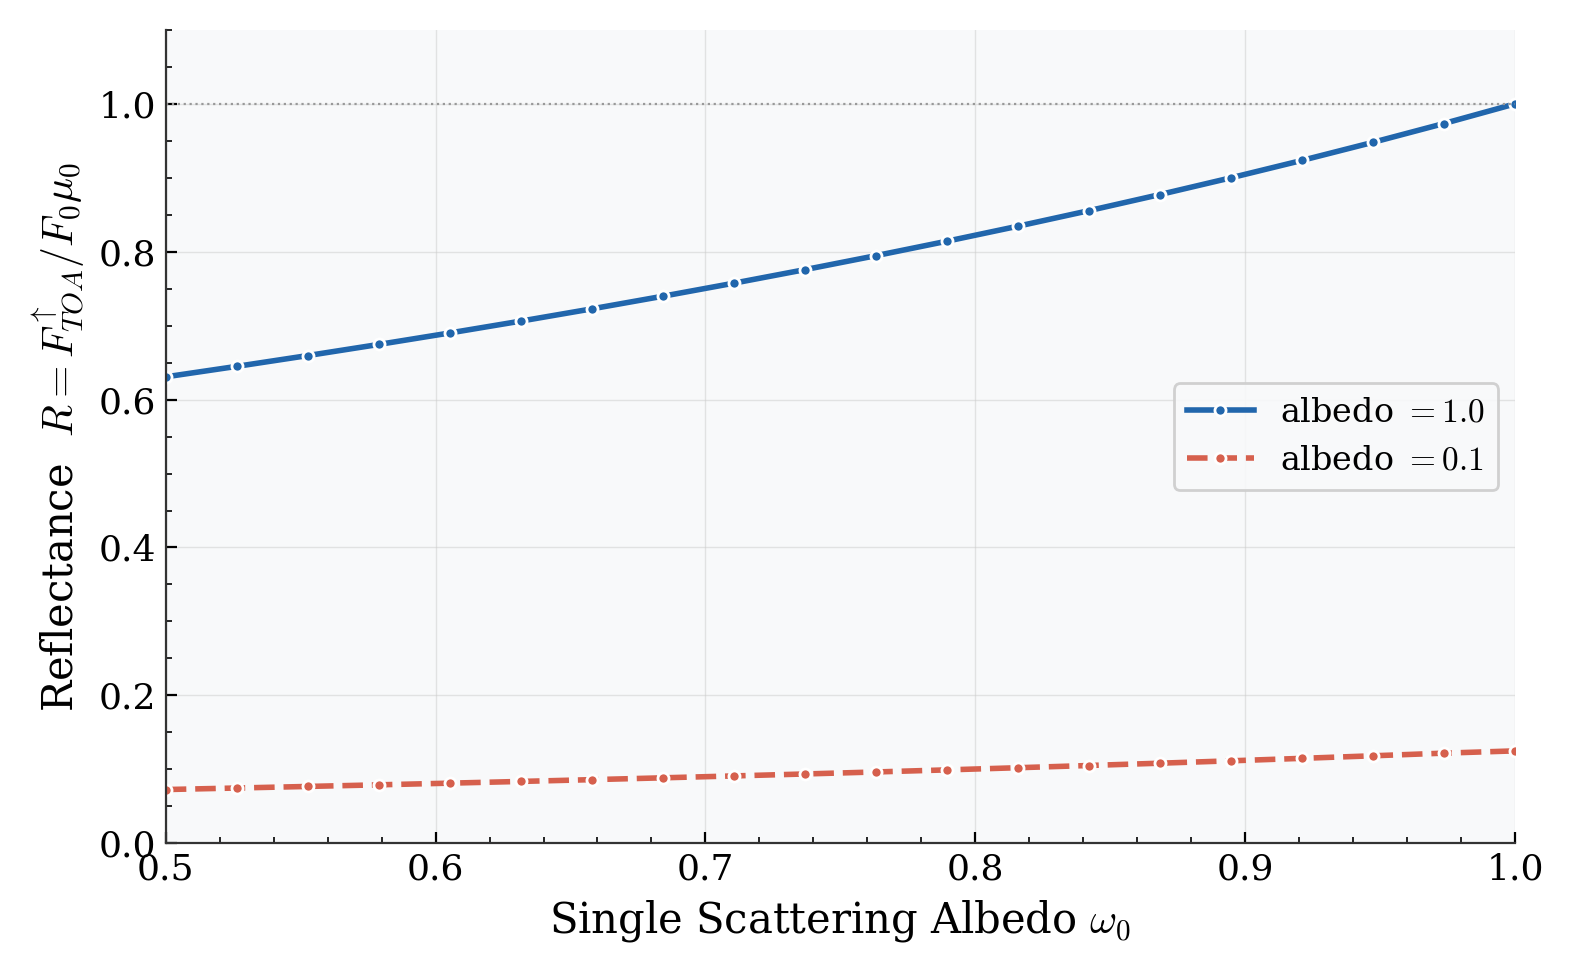
\includegraphics[width=0.49\textwidth]{Images_final_report/Level1_energy_conservation_AOD_03_g07_N36_theta030.png}%
	\hfill
	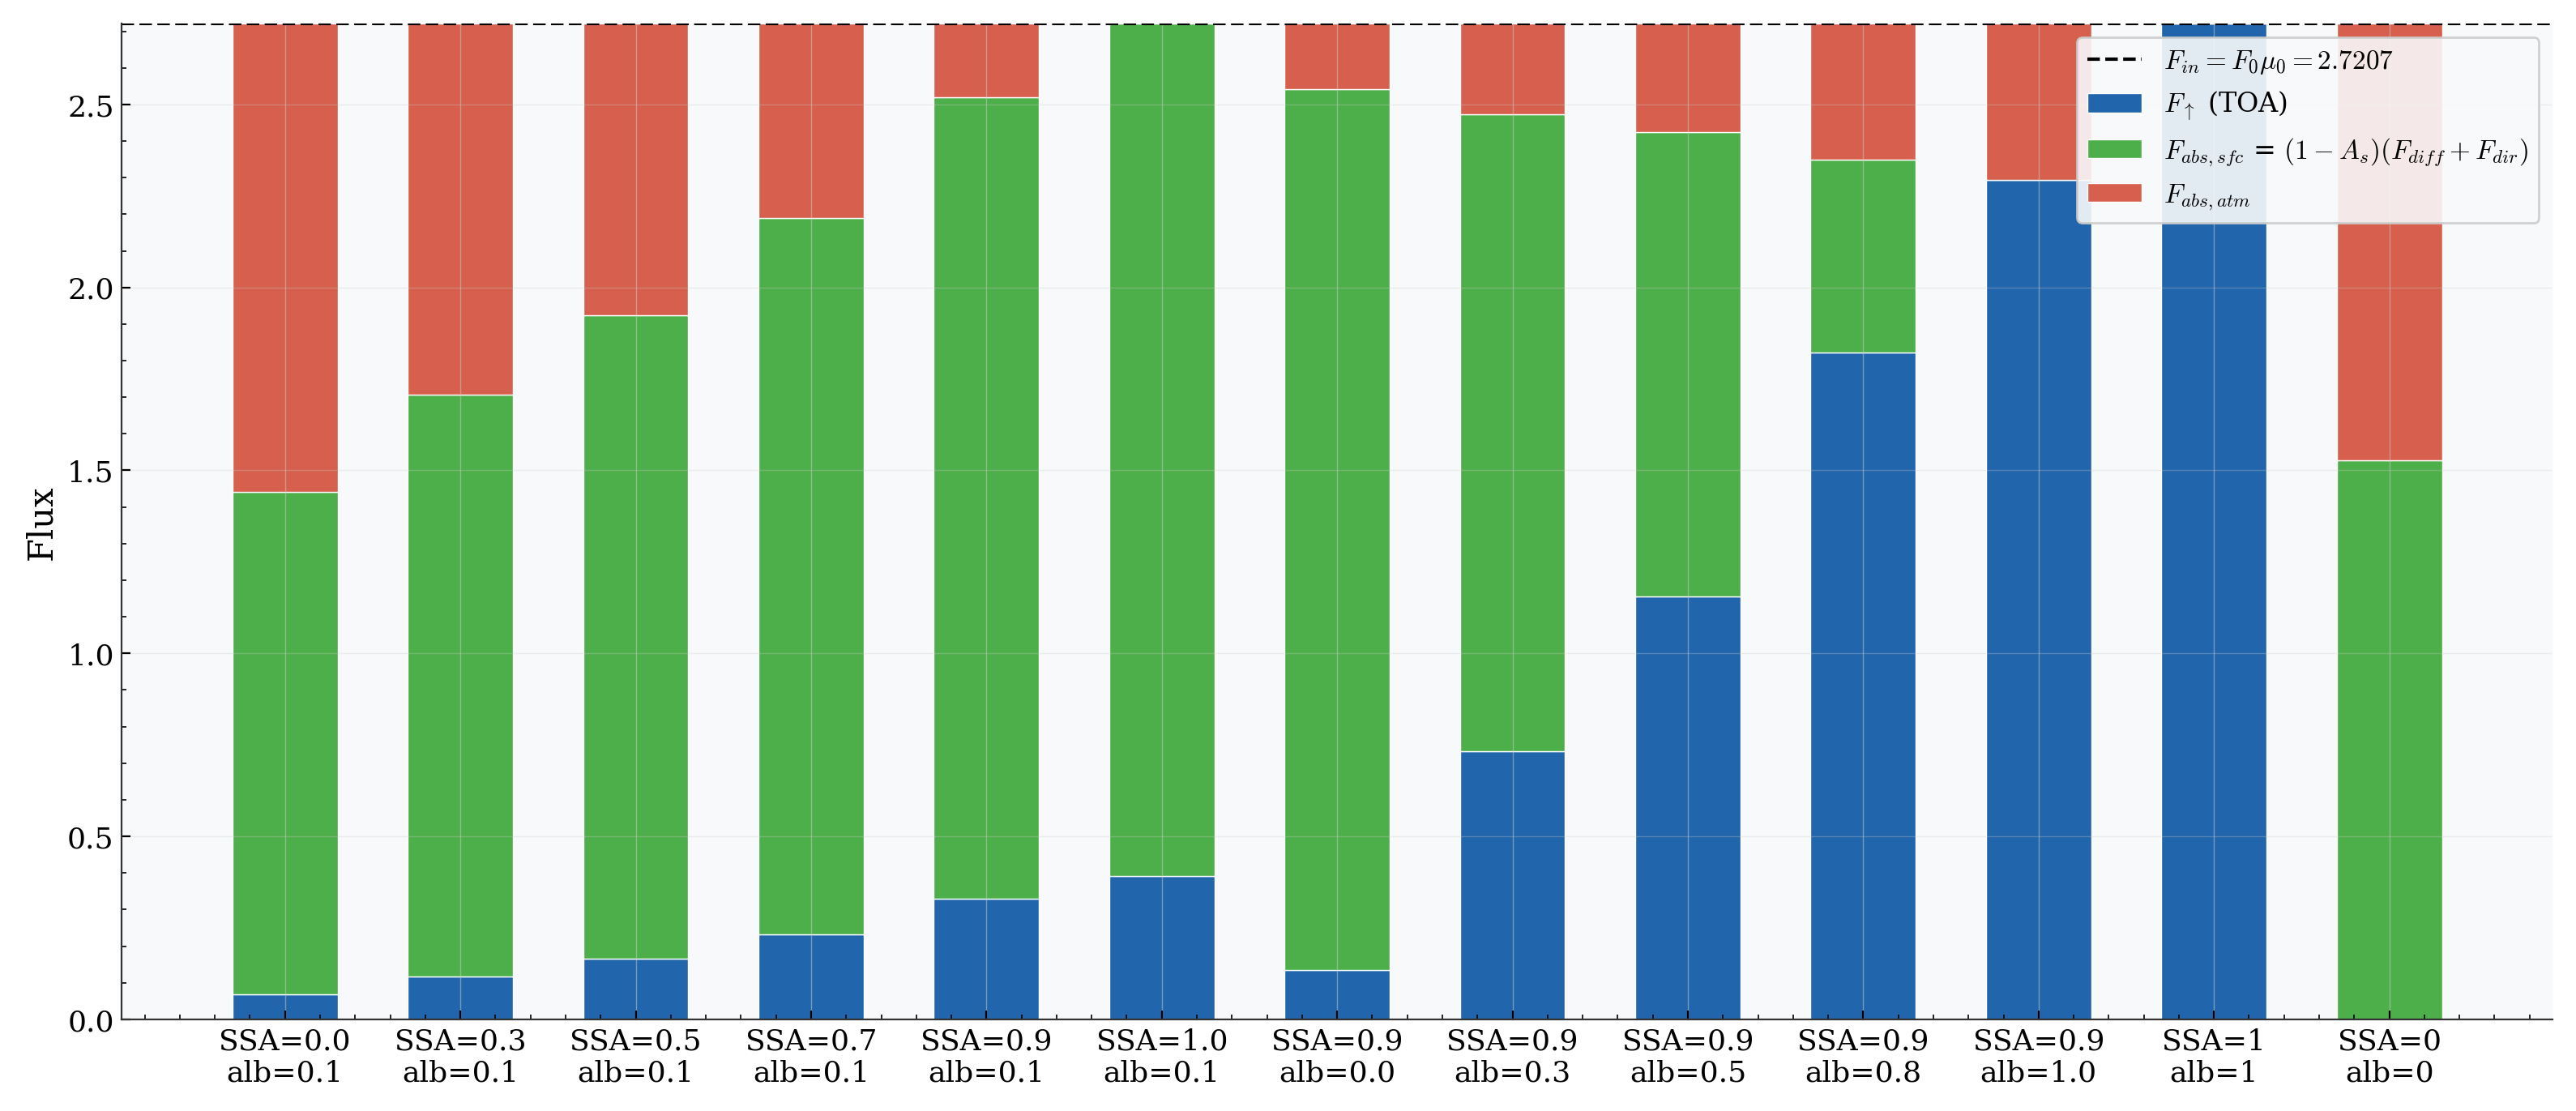
\includegraphics[width=0.49\textwidth]{Images_final_report/Energy_balance_AOD_05_N36_theta030.png}
	\caption{a)~TOA reflectance $R = F_{\mathrm{TOA}}^{\uparrow}/F_0\mu_0$ as a function of single scattering albedo $\omega_0$ for two surface albedo values. $\tau=0.3$, $g=0.7$, $N=36$ streams, $\theta_0=30^{\circ}$.
	b)~Stacked energy budget for a single-layer atmosphere ($\tau=0.5$, $g=0.7$, $N=36$ streams, $\theta_0=30^{\circ}$).
	Each bar decomposes the incoming flux $F_{\mathrm{in}}=F_0\mu_0=2.7207$ (dashed line) into three components:
	upwelling flux at TOA ($F_{\uparrow}$, blue), surface absorption ($F_{\mathrm{abs,sfc}}=(1-A_s)(F_{\mathrm{diff}}+F_{\mathrm{dir}})$, green),
	and atmospheric absorption ($F_{\mathrm{abs,atm}}$, red).
	Left group: SSA sweep at $A_s=0.1$; centre group: albedo sweep at $\omega_0=0.9$; right: limiting cases ($\omega_0=1,A_s=1$ and $\omega_0=0,A_s=0$).}
	\label{fig:energy_tests}
\end{figure}

\subsection{Discrete vs Continuous Solution}

\begin{figure}[H]
	\centering
	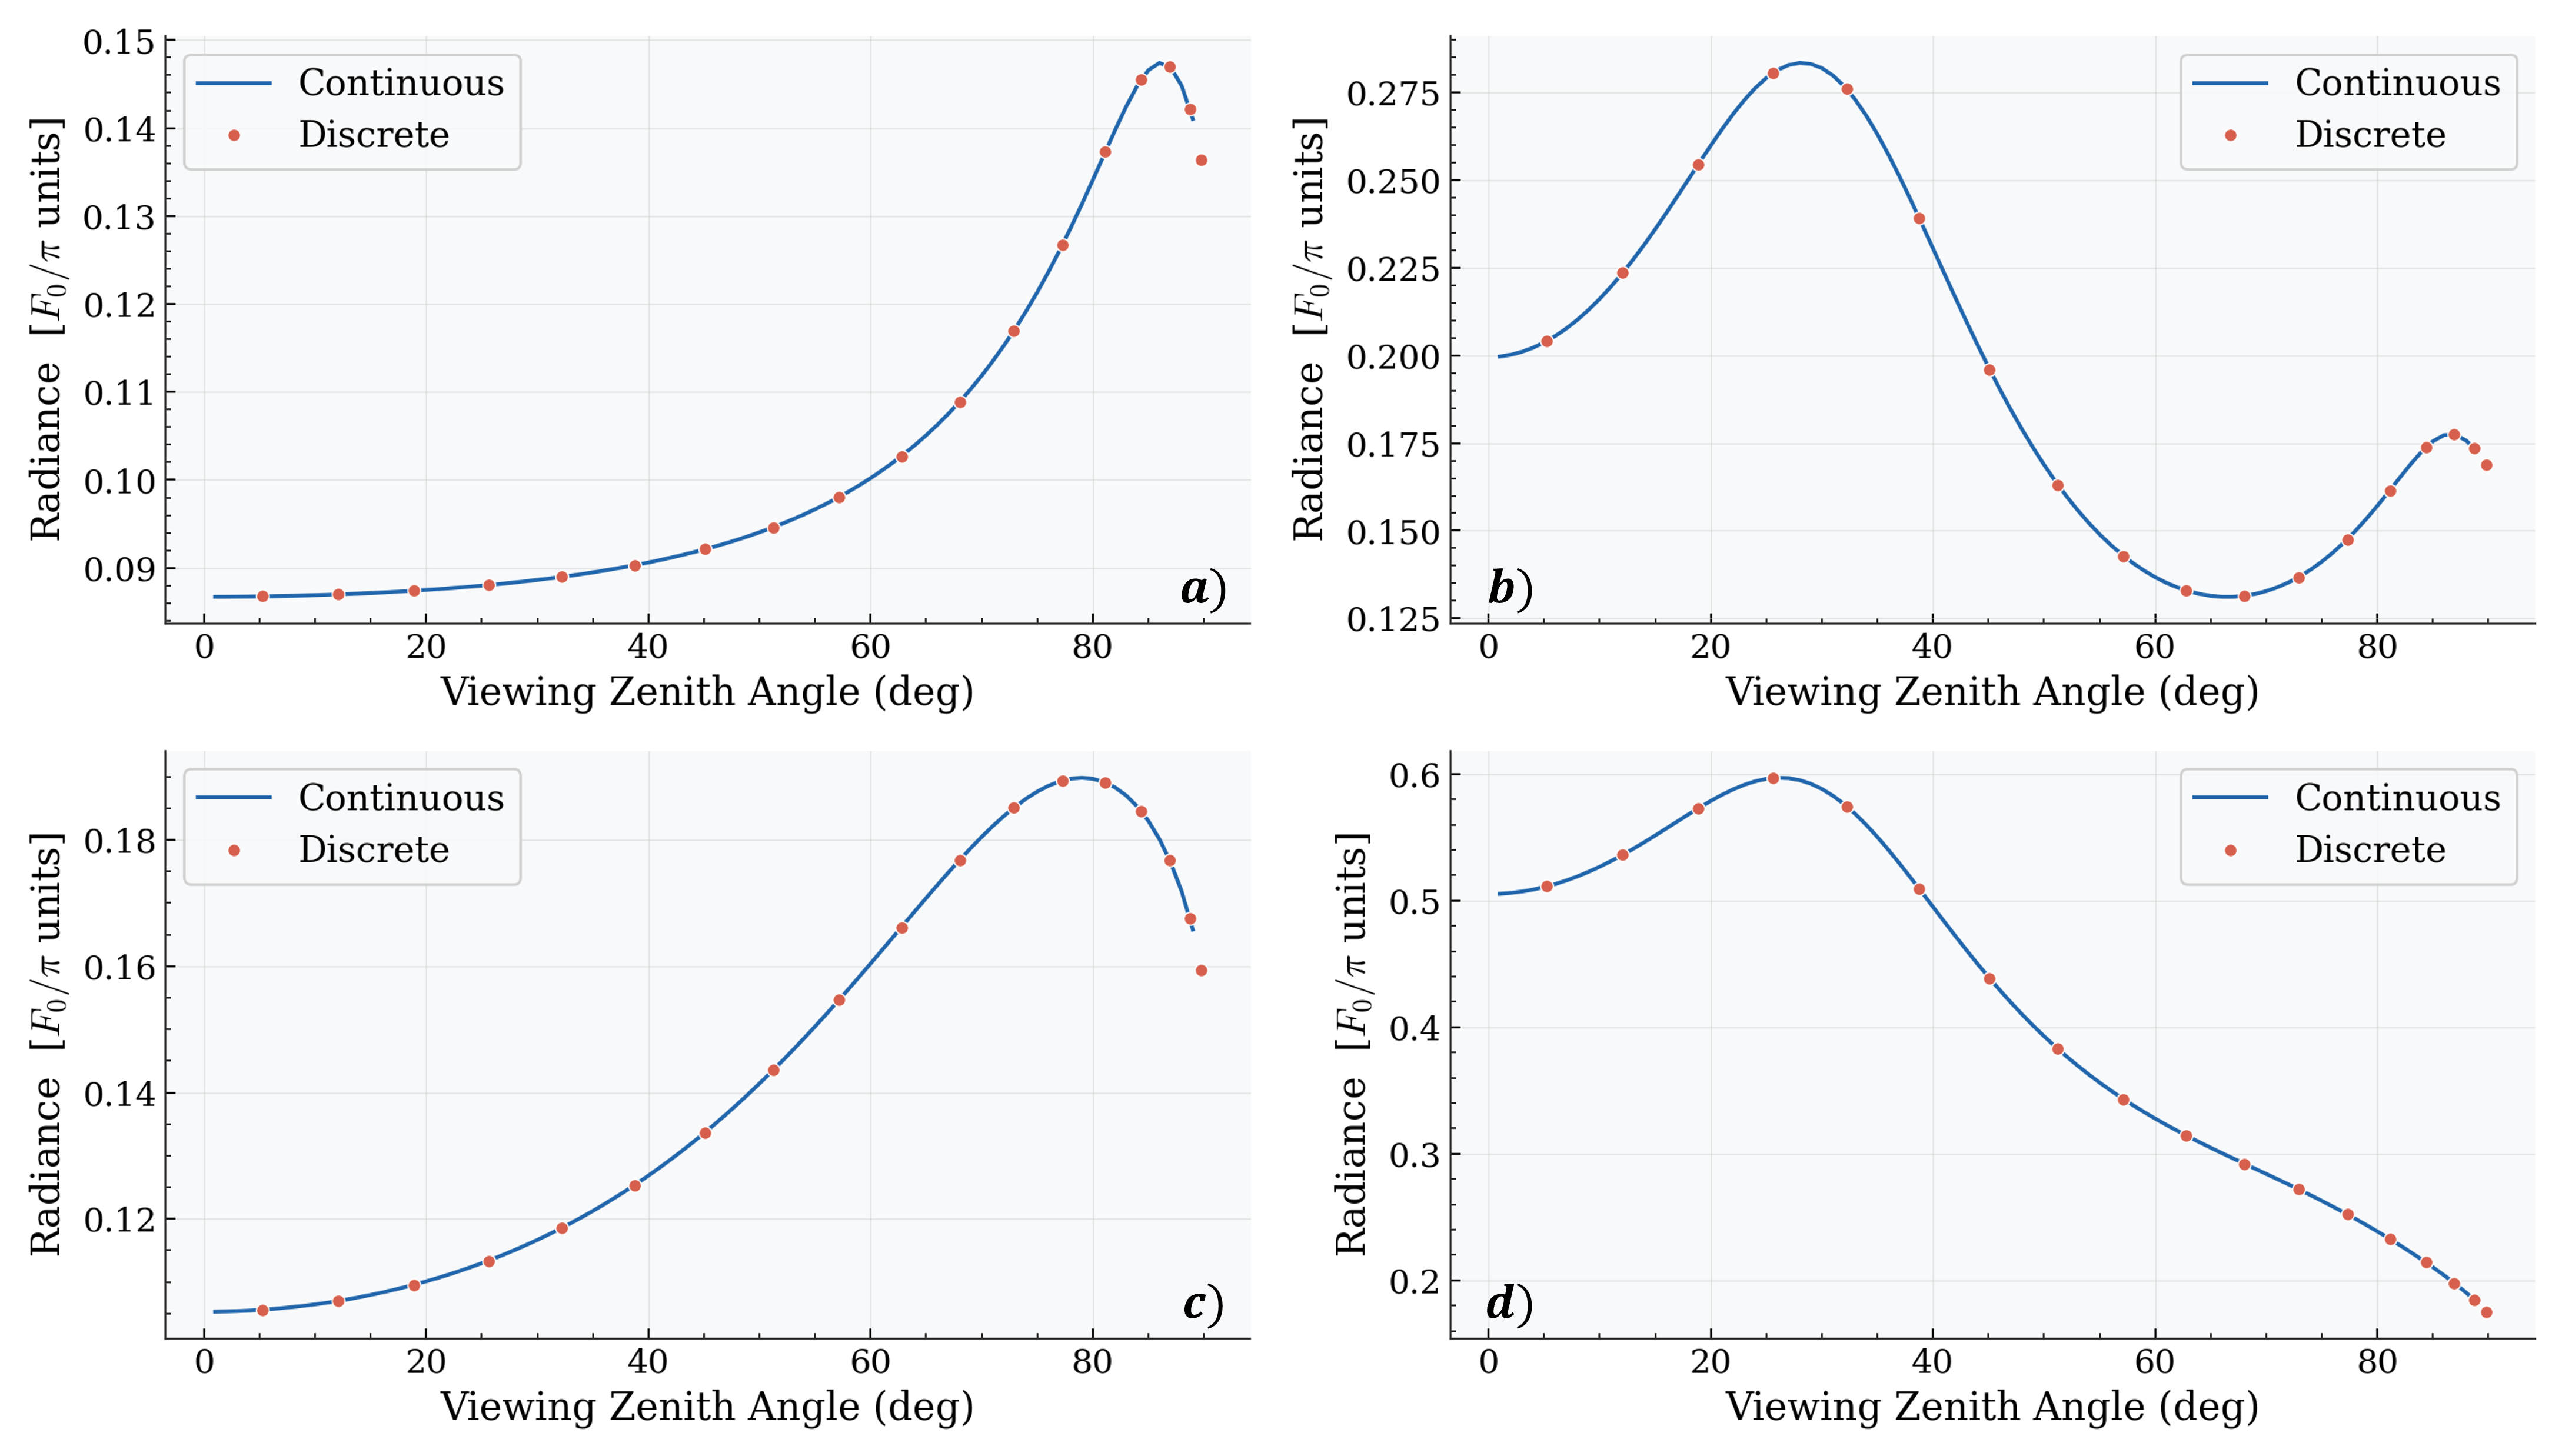
\includegraphics[width=0.7\textwidth]{Images_final_report/Discrete_vs_continuous_N36_theta030.png}
	\caption{Comparison between the discrete solution (Eq.~\ref{eq:general_solution}, dots) evaluated at the $N/2$ quadrature nodes and the continuous source-function interpolation (Eq.~\ref{eq:intensity_toa}, solid lines) evaluated at $1^{\circ}$ angular resolution.
	$N=36$ streams, $\theta_0=30^{\circ}$, delta-M scaling OFF.
	(a)~TOA upwelling, baseline scenario: $\tau=0.3$, $\omega_0=0.9$, $g=0.7$, $A_s=0.1$.
	(b)~BOA downwelling, baseline scenario.
	(c)~TOA upwelling, high AOD scenario: $\tau=1.5$, $\omega_0=0.9$, $g=0.7$, $A_s=0.1$.
	(d)~BOA downwelling, high AOD scenario.}
	\label{fig:discrete_vs_continuous}
\end{figure}

Figure~\ref{fig:discrete_vs_continuous} validates the source-function
interpolation (Eqs.~\ref{eq:formal_up}--\ref{eq:formal_down})
against the discrete solution at the quadrature nodes.  In all four
panels, the interpolated curve passes through the discrete points
with machine-precision agreement, confirming the interpolatory
property of the method \cite{stamnes1982}.  The continuous curves
reveal the full angular structure that the $N/2 = 18$ discrete points
can only sample: all TOA upwelling profiles (panels~a and~c) exhibit
the characteristic horizon enhancement discussed in
Eq.~\eqref{eq:horizon_saturation}.  At TOA for the baseline case
(panel~a), the radiance increases monotonically from ${\sim}0.09$ at
nadir to ${\sim}0.14$ at the horizon.  For the high-AOD case
(panel~c), a local intensity maximum appears near
$\theta_v \approx 60^{\circ}$--$70^{\circ}$ followed by a slight
decrease close to $90^{\circ}$.  This behaviour arises because at
very high $\tau$, the competition between the growing source-function
contribution and the exponential extinction of the surface-reflected
component $I_{\text{surf}}\,e^{-\tau_L/\mu}$ (which decays rapidly
as $\mu \to 0^+$) creates a turning point: beyond a critical angle,
the loss of the surface term outweighs the gain from atmospheric
scattering.  At BOA (panels~b and~d), the forward-scattering peak
near $\theta_v \approx 30^{\circ}$ is clearly resolved by the
interpolation but is only coarsely sampled by the discrete points,
illustrating the practical necessity of the source-function technique
for obtaining physically meaningful angular distributions.

\subsection{Extreme Physical Cases}

\begin{figure}[H]
	\centering
	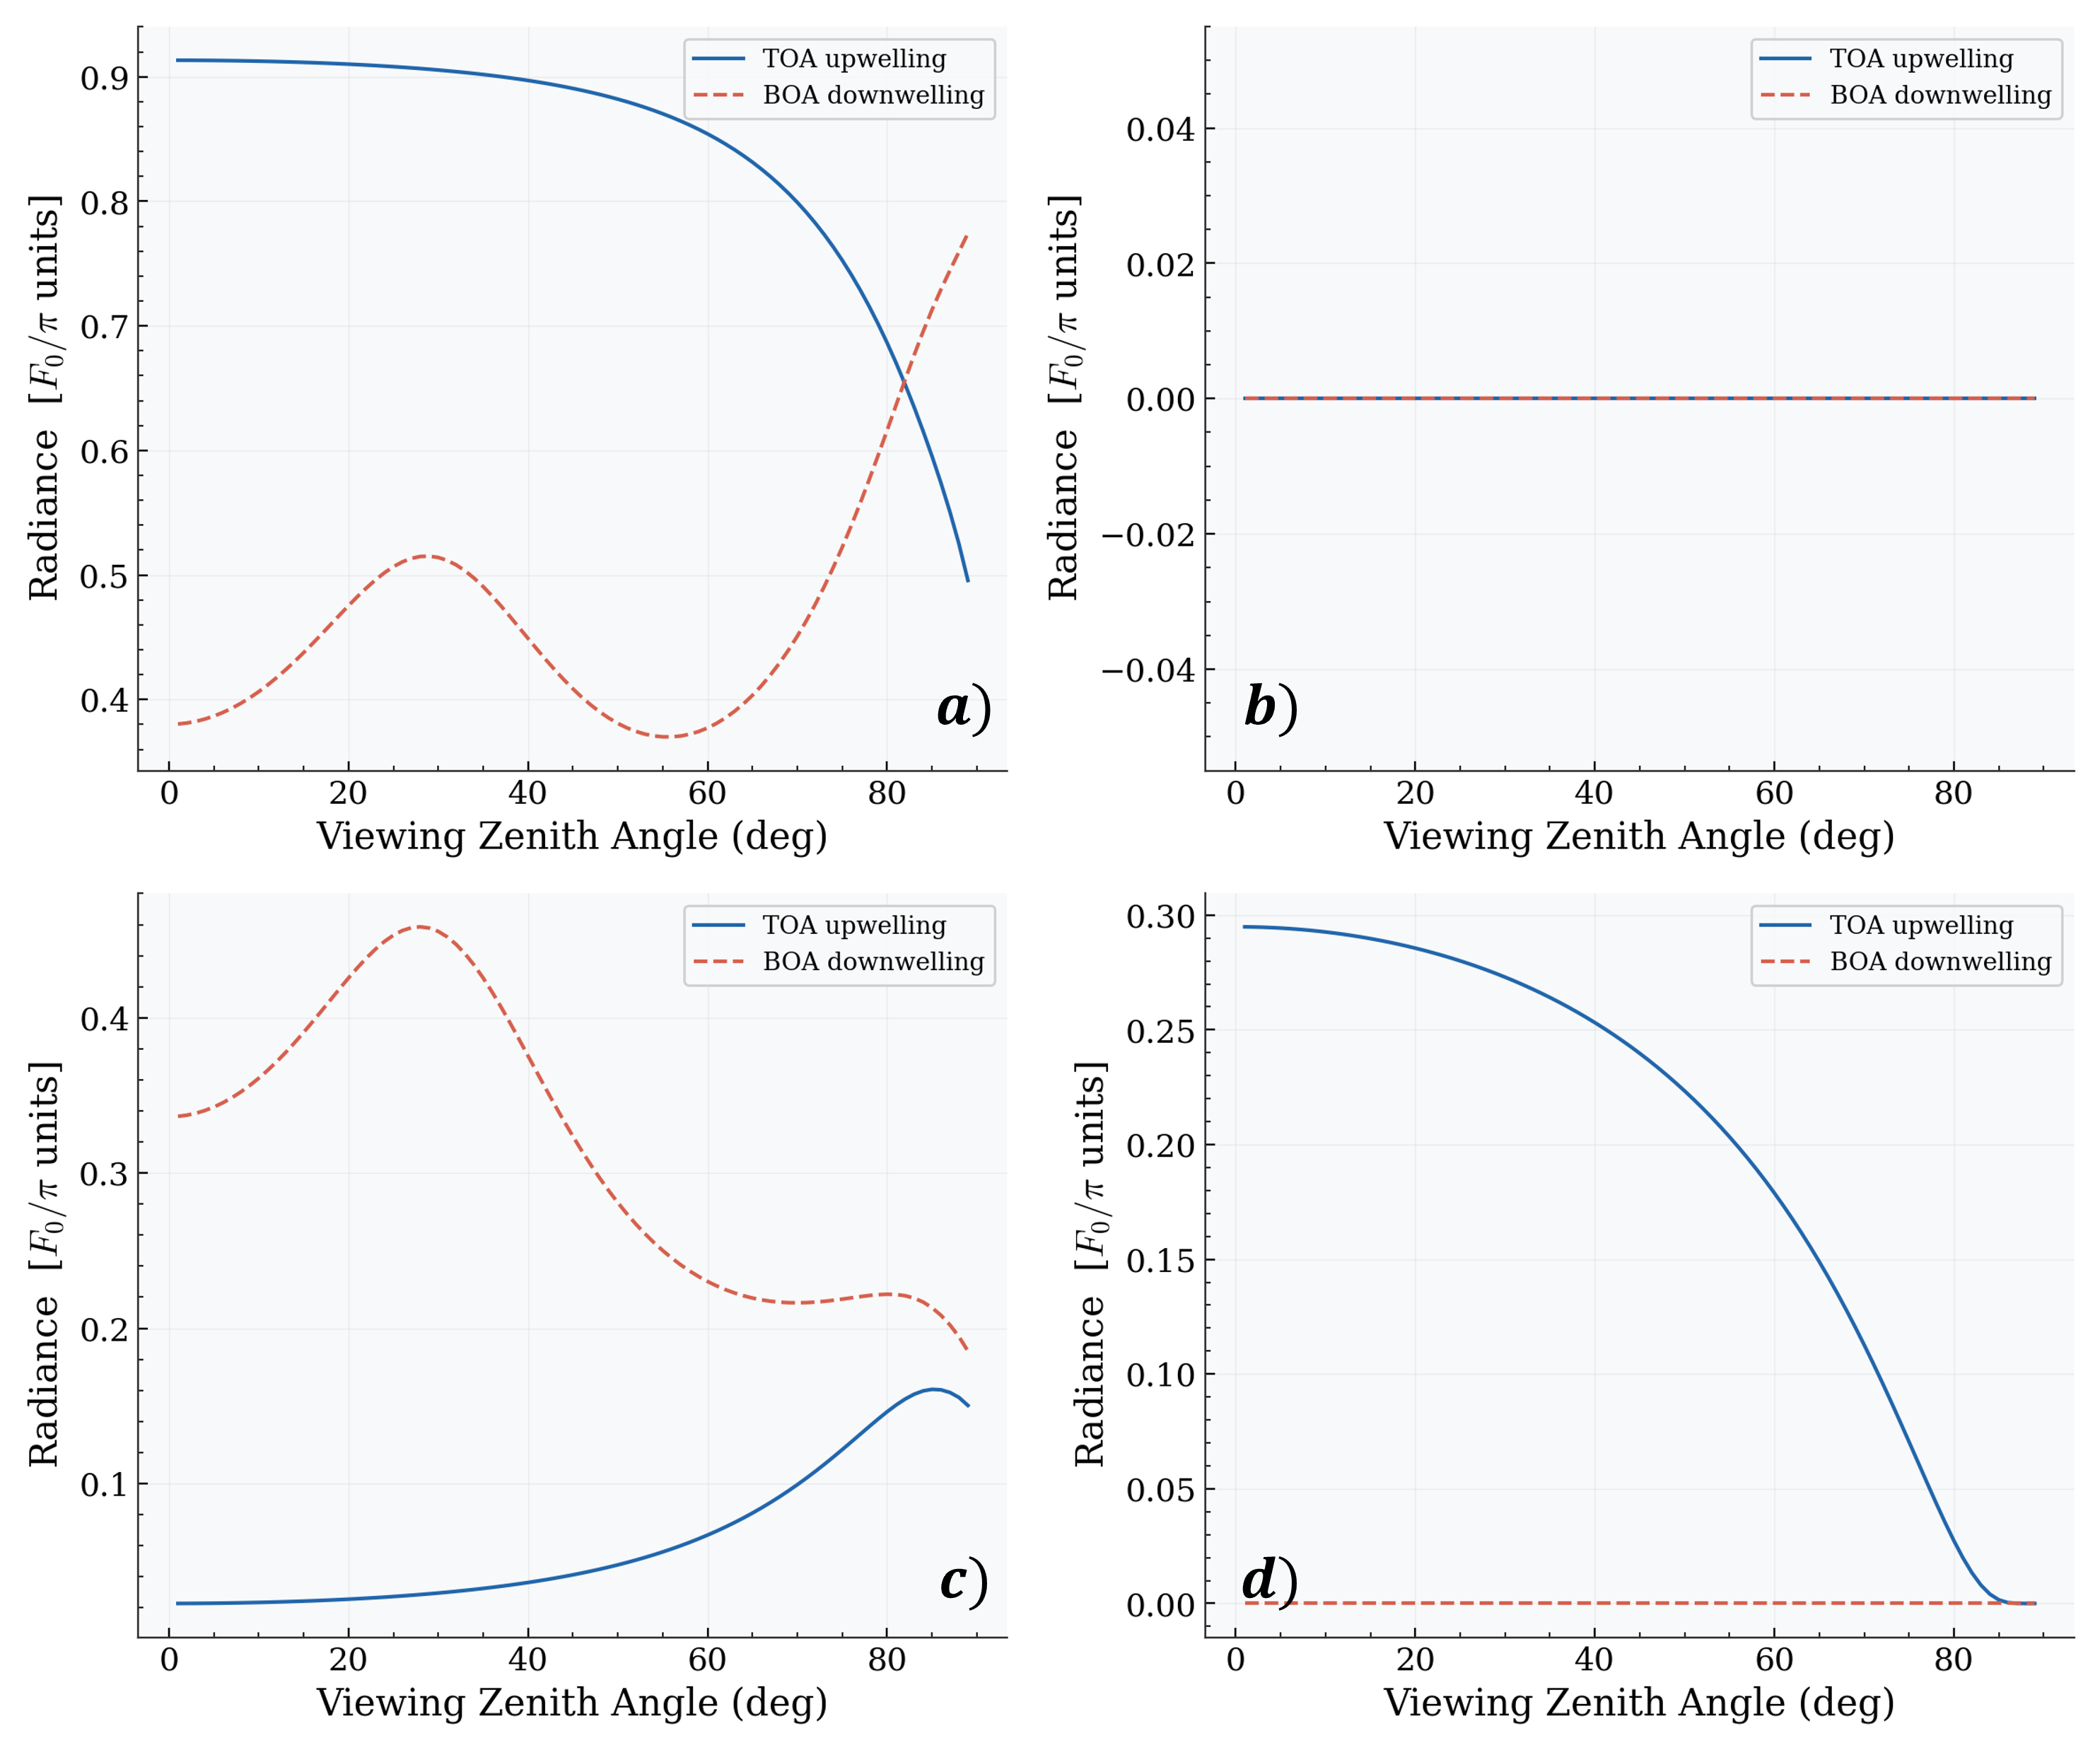
\includegraphics[width=0.7\textwidth]{Images_final_report/Extreme_cases_AOD_05_N36_theta030.png}
	\caption{Radiance fields (TOA upwelling and BOA downwelling) for four limiting physical scenarios.
	All cases: $\tau=0.5$, $N=36$ streams, $\theta_0=30^{\circ}$.
	(a)~$\omega_0=1$, $A_s=1$.
	(b)~$\omega_0=0$, $A_s=0$.
	(c)~$\omega_0=1$, $A_s=0$.
	(d)~$\omega_0=0$, $A_s=1$.}
	\label{fig:extreme_cases}
\end{figure}

Figure~\ref{fig:extreme_cases} tests the model at four extreme
combinations of $\omega_0$ and $A_s$.

\textbf{Panel~(a)} ($\omega_0 = 1$, $A_s = 1$): conservative
scattering with a perfect reflector.  The TOA radiance is the highest
of all cases (${\sim}0.90$ at nadir) and \emph{decreases} towards the
horizon.  This decrease occurs because the dominant signal is the
surface-reflected flux transmitted through the atmosphere:
$I_{\text{surf}} \propto A_s\,e^{-\tau/\mu}$, and as $\mu \to 0^+$
this transmission factor vanishes.  Meanwhile the scattering source
function is also saturated ($\omega_0 = 1$), but the isotropic surface
reflection provides more intensity than atmospheric scattering can at
near-nadir angles.  The competition between these two contributions
produces the observed decrease.  The BOA curve increases towards the
horizon due to the atmospheric scattering path-length effect.

\textbf{Panel~(b)} ($\omega_0 = 0$, $A_s = 0$): pure absorption
with a black surface.  Both TOA and BOA radiances are identically
zero, as physically expected: no scattering means no source function
($S = 0$), and no surface reflection means $I_{\text{surf}} = 0$.

\textbf{Panel~(c)} ($\omega_0 = 1$, $A_s = 0$): conservative
scattering with a black surface.  The TOA radiance increases towards
the horizon, following the pure atmospheric scattering pattern of
Eq.~\eqref{eq:horizon_saturation} without any competing surface
contribution.  The BOA curve shows a forward-scattering peak near
$\theta_v \approx 30^{\circ}$.

\textbf{Panel~(d)} ($\omega_0 = 0$, $A_s = 1$): pure absorption with
a perfect reflector.  The TOA radiance is entirely due to the
surface-reflected beam attenuated by two passages through the
atmosphere (down and up):
$I_{\text{TOA}} \propto A_s\,e^{-\tau/\mu_0}\,e^{-\tau/\mu}$.  Since
$\omega_0 = 0$, there is no scattering contribution, and the intensity
decreases monotonically from nadir ($\mu = 1$,
$I \propto e^{-\tau}$) to the horizon ($\mu \to 0^+$, $I \to 0$).
The BOA downwelling radiance is nearly zero because there is no
atmospheric scattering to redirect photons downward.

\subsection{Level~1: Single-Layer AOD Retrieval}

\begin{figure}[H]
	\centering
	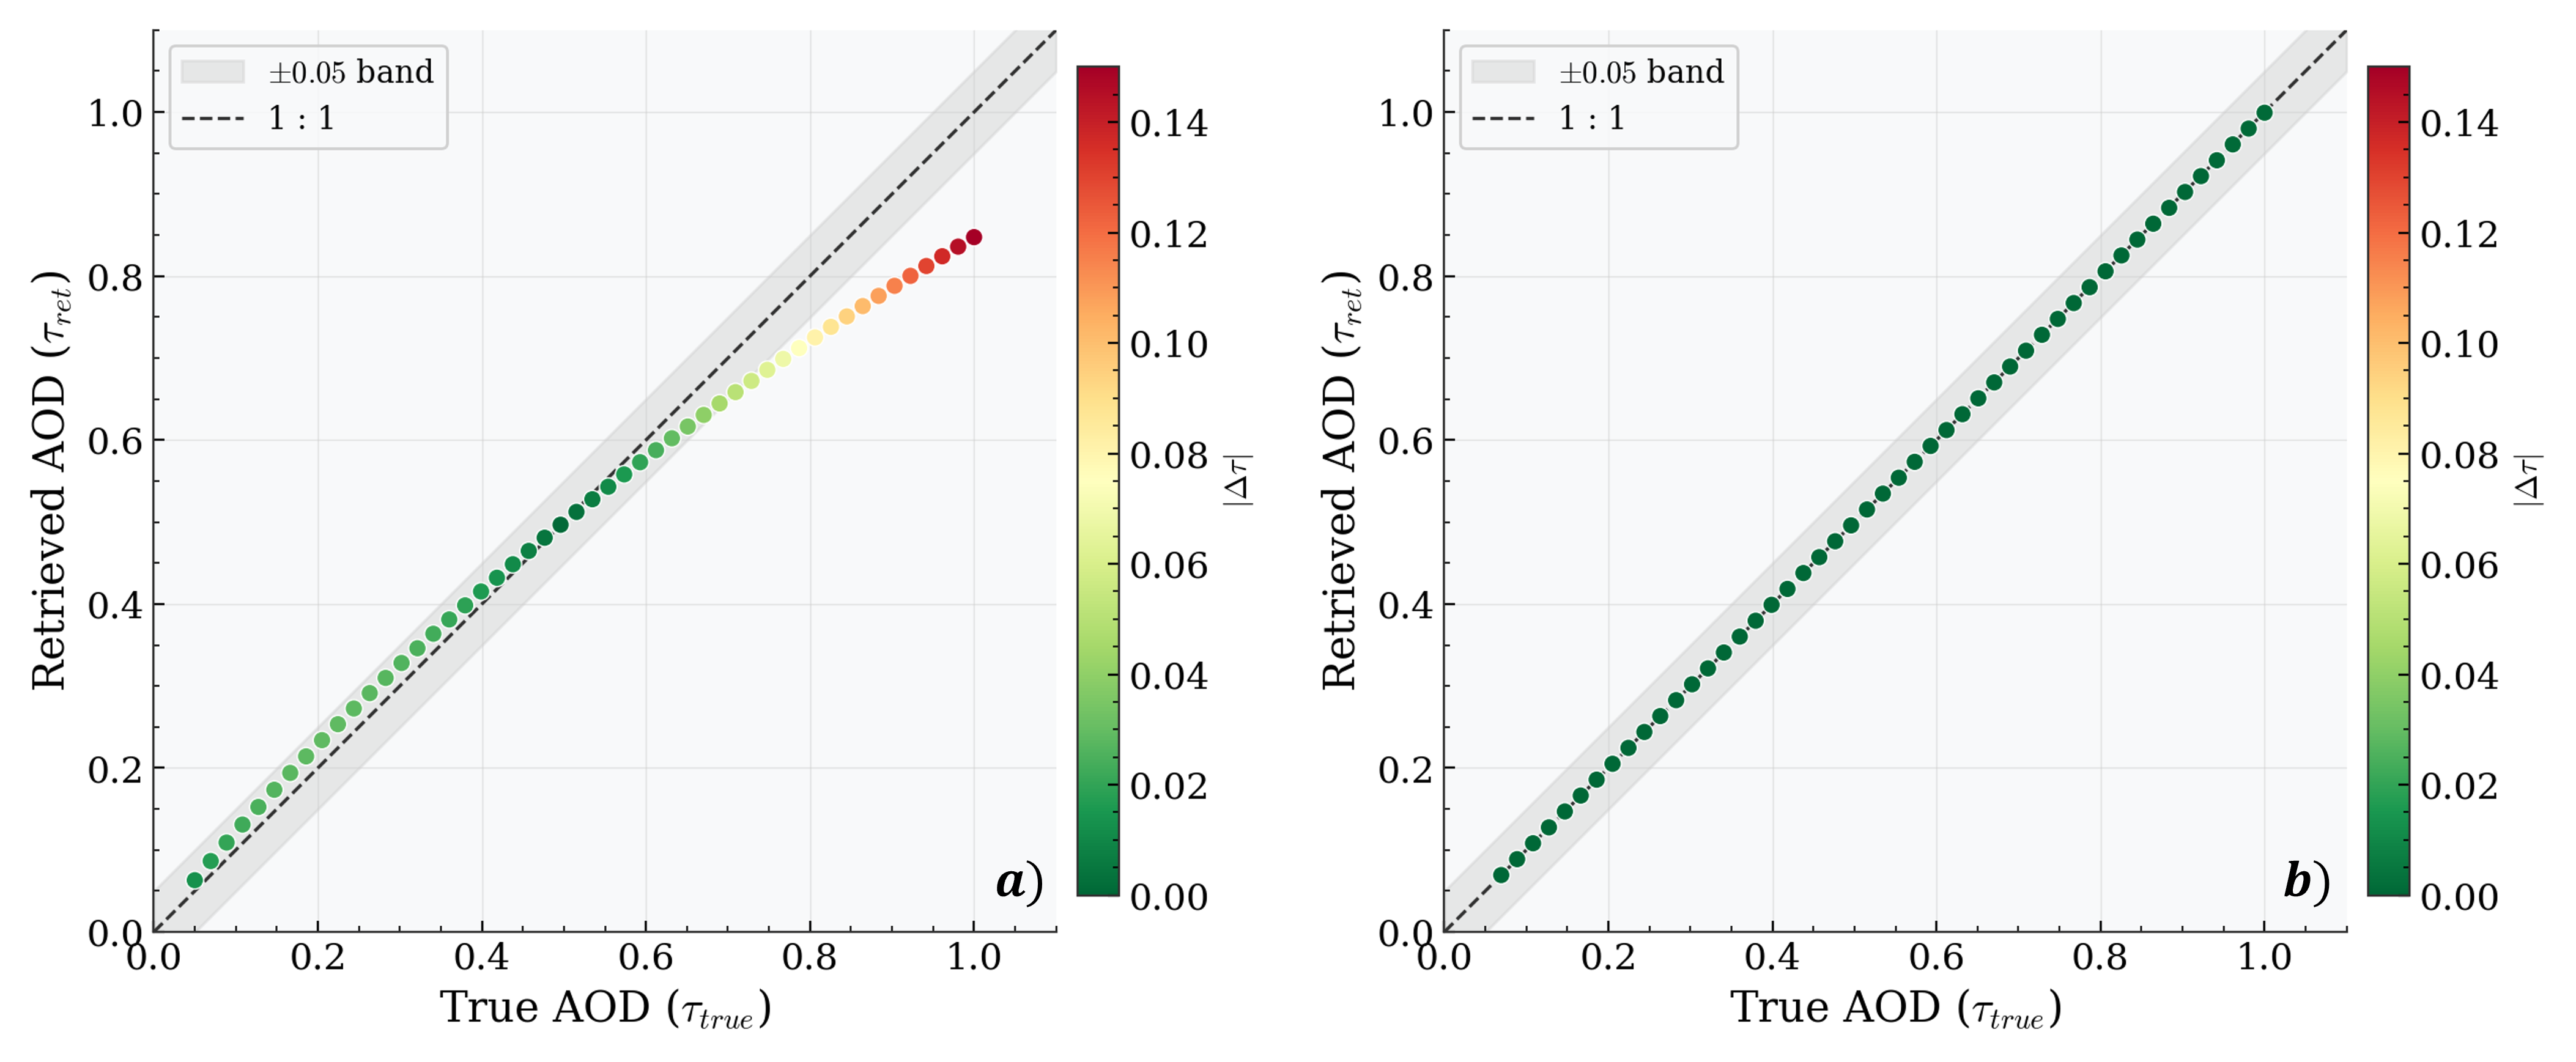
\includegraphics[width=0.7\textwidth]{Images_final_report/Level1_AOD_scatter_SSA_09_g07_N36_theta030.png}
	\caption{AOD retrieval scatter plots for a single homogeneous layer ($\omega_0=0.9$, $g=0.7$, $A_s=0.1$, $N=36$ streams, $\theta_0=30^{\circ}$).
	a)~Levenberg--Marquardt with Tikhonov regularisation
	b)~Optimal Estimation (Rodgers)}
	\label{fig:level1_aod}
\end{figure}

Figure~\ref{fig:level1_aod} compares the two retrieval methods for
the single-layer case, where the only unknown is the aerosol optical
depth~$\tau$.  The OE method (panel~b) recovers the true AOD with
negligible bias across the full range $\tau \in [0, 1]$, with all
points falling on the 1:1 line within the $\pm0.05$ band.  The
LM+Tikhonov method (panel~a) performs comparably for $\tau \lesssim
0.5$ but develops a systematic low bias at higher optical depths: the
retrieved AOD saturates below the true value, with the colour scale
indicating absolute errors $|\Delta\tau| > 0.10$ for $\tau > 0.7$.
This degradation arises because the Tikhonov penalty
(Eq.~\ref{eq:cost_tikh}) pulls the solution towards the a~priori
$\tau_a = 0.5$ with a strength proportional to~$\gamma$, and this
regularisation bias grows as the true state moves further from
$\mathbf{x}_a$.  In contrast, the OE formulation
(Eq.~\ref{eq:cost_oe}) weights the a~priori constraint by the inverse
covariance~$\mathbf{S}_a^{-1}$, allowing the data to dominate when
the measurements are informative.

\subsection{Level~2: 20-Layer Joint Retrieval}

\begin{figure}[H]
	\centering
	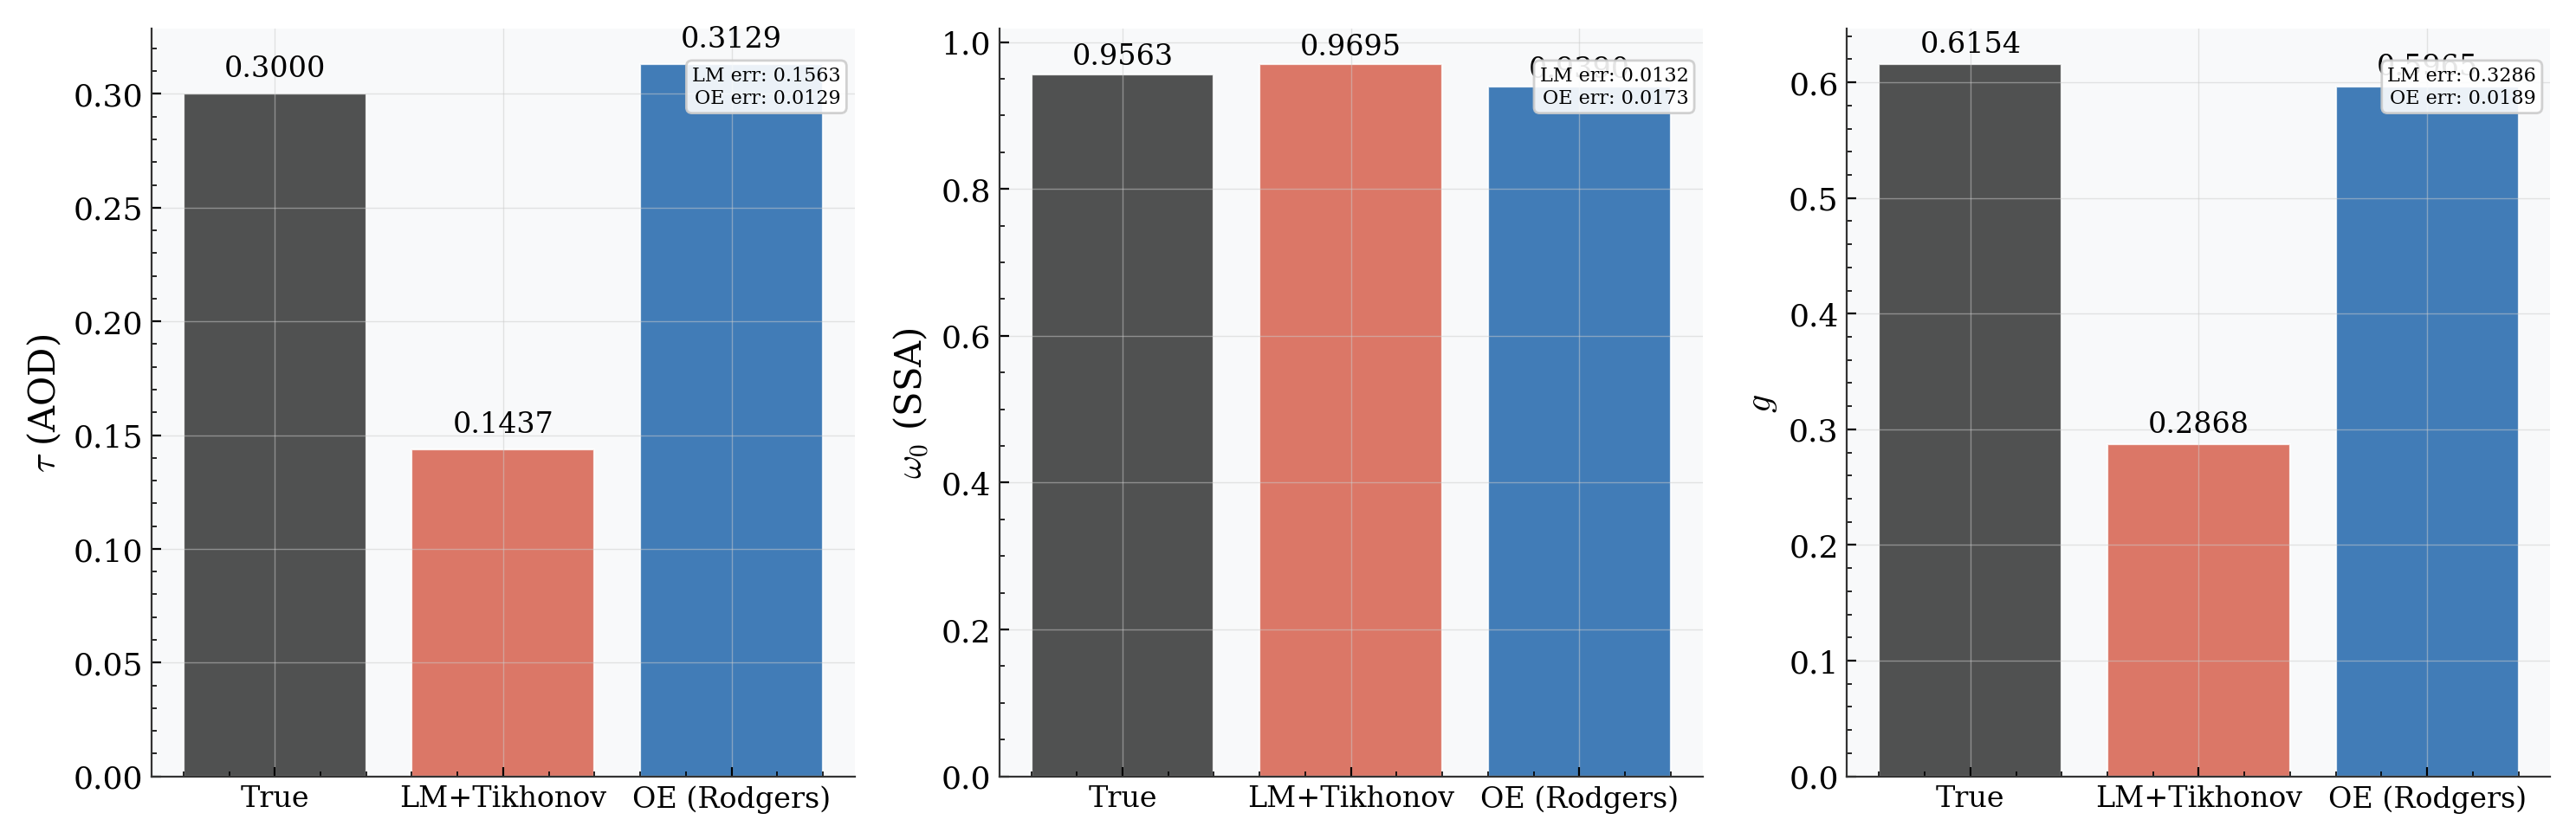
\includegraphics[width=\textwidth]{Images_final_report/Level2_LM_vs_OE_continental_AOD_03_N36_theta030.png}
	\caption{Comparison of retrieved aerosol parameters between LM+Tikhonov and Optimal Estimation (Rodgers) for a 20-layer continental aerosol atmosphere.
	True values: $\tau=0.300$, $\omega_0=0.9563$, $g=0.6154$.
	$N=36$ streams, $\theta_0=30^{\circ}$.
	(a)~AOD ($\tau$), (b)~single scattering albedo ($\omega_0$), (c)~asymmetry parameter ($g$).}
	\label{fig:level2_lm_vs_oe}
\end{figure}

\begin{figure}[H]
	\centering
	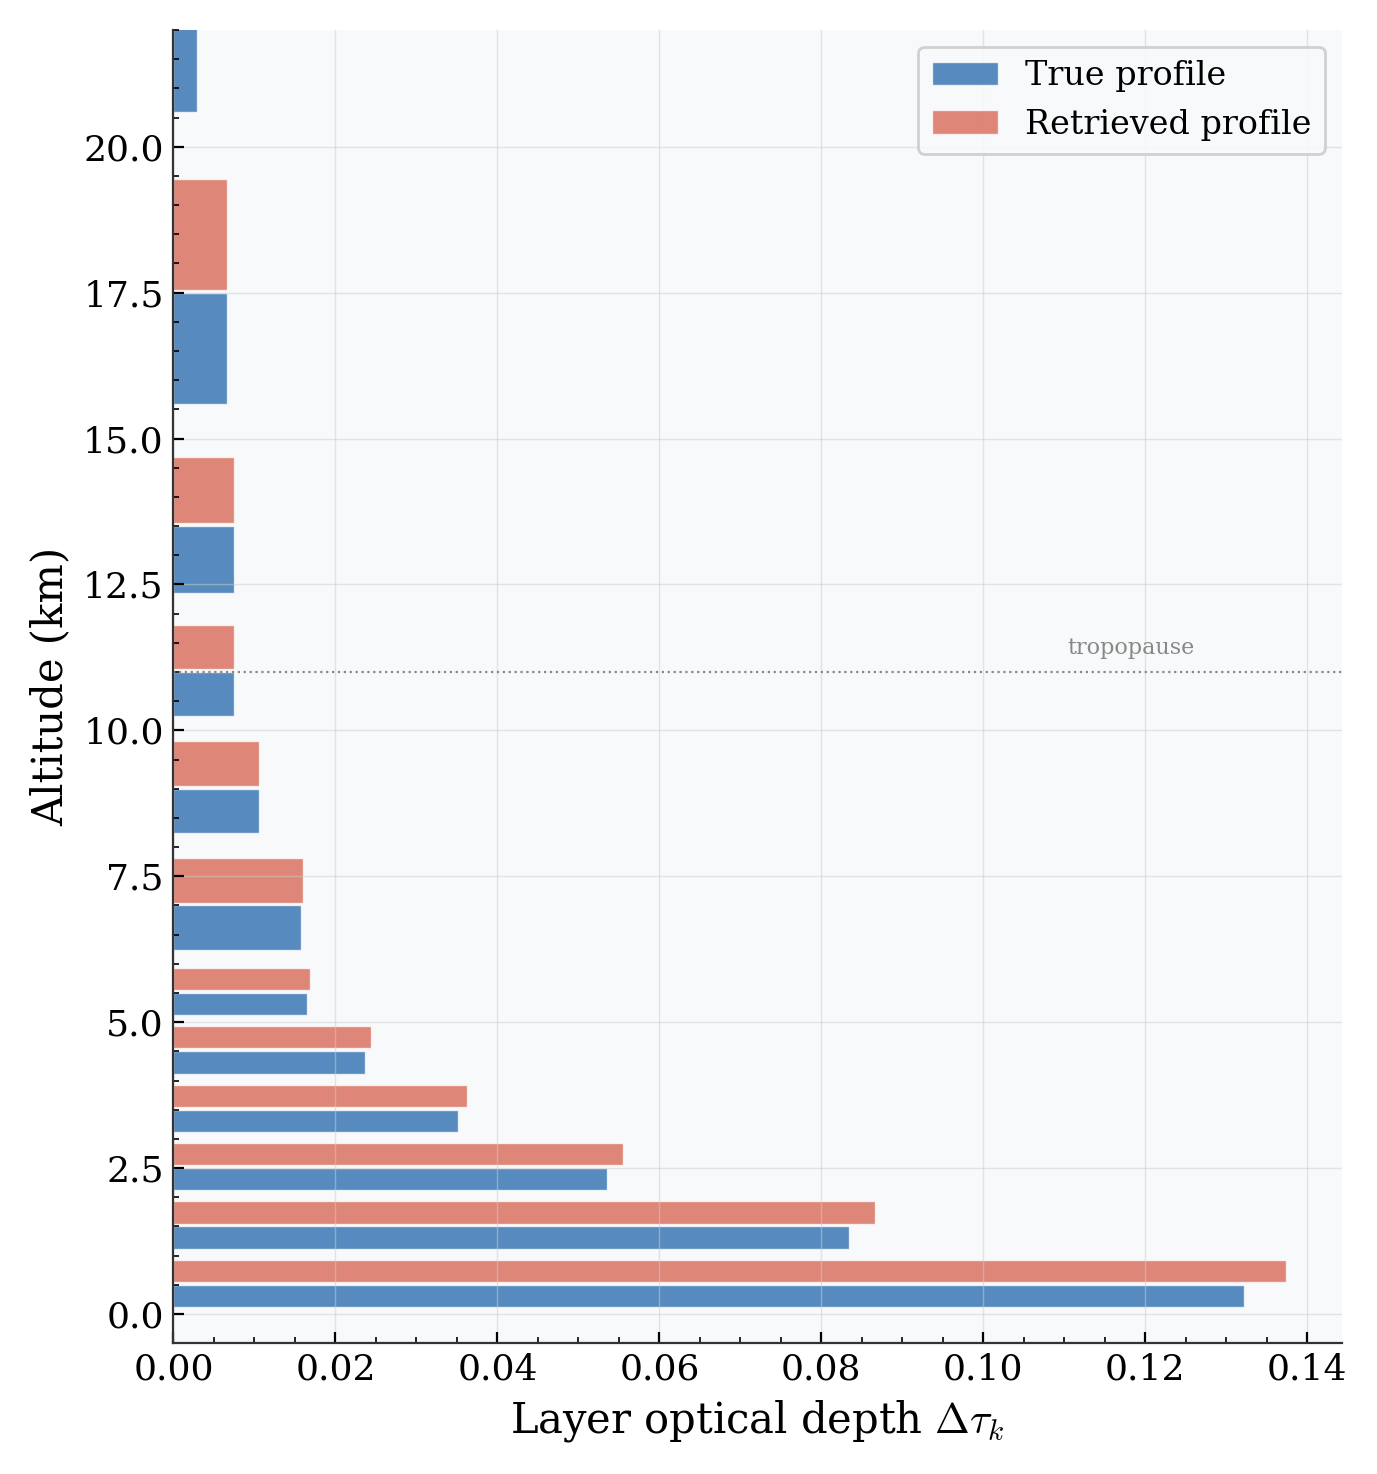
\includegraphics[width=0.5\textwidth]{Images_final_report/Level2_vertical_profile_continental_AOD_03_N36.png}
	\caption{Vertical profile of layer optical depth $\Delta\tau_k$ for the 20-layer atmosphere: true profile (blue) vs OE-retrieved profile (red).
	Continental aerosol type, $\tau_{\mathrm{total}}^{\mathrm{true}}=0.300$, $\tau_{\mathrm{total}}^{\mathrm{ret}}=0.313$.}
	\label{fig:level2_vertical}
\end{figure}

The joint retrieval of three parameters ($\tau$, $\omega_0$, $g$) in a
realistic 20-layer atmosphere (Figures~\ref{fig:level2_lm_vs_oe}
and~\ref{fig:level2_vertical}) reveals a marked difference between the
two methods.  The OE retrieval recovers all three parameters with
errors below 5\%: $\tau_{\text{ret}} = 0.3129$ (true: 0.300, error
4.3\%), $\omega_{0,\text{ret}} = 0.9695$ (true: 0.9563, error
1.4\%), and $g_{\text{ret}} = 0.6343$ (true: 0.6154, error 3.1\%).
In contrast, the LM+Tikhonov method severely underestimates the AOD
($\tau_{\text{ret}} = 0.1437$, error 52\%) and the asymmetry parameter
($g_{\text{ret}} = 0.2868$, error 53\%), while retrieving a
reasonable SSA.  This failure illustrates the well-known trade-off
between $\tau$ and $g$ in the inverse problem
\cite{rodgers2000}: an increase in $\tau$ combined with
an increase in $g$ can produce nearly identical TOA radiance fields,
because forward-scattering aerosols redirect less energy towards the
observer and thus partially compensate the effect of increased
extinction.  The scalar Tikhonov regularisation cannot resolve this
degeneracy, whereas the OE method exploits the full covariance
structure~$\mathbf{S}_a$ to constrain the coupled parameters.

The vertical profile (Figure~\ref{fig:level2_vertical}) confirms that
the OE retrieval preserves the exponential decrease with altitude
prescribed by the aerosol scale height $H_{\text{aer}} = 2$~km
(Eq.~\ref{eq:aer_profile}).  The retrieved column total
($\tau_{\text{ret}} = 0.313$) overestimates the truth ($\tau = 0.300$)
by only 4.3\%, and the layer-by-layer structure is well reproduced
below 5~km, where the bulk of the aerosol loading resides.  Above
the tropopause ($z > 11$~km), both profiles converge to the Rayleigh
background, indicating that the retrieval correctly attributes the
upper-atmosphere optical depth to molecular scattering alone.

\subsection{Level~3: Real-Data Retrieval}

\begin{figure}[H]
	\centering
	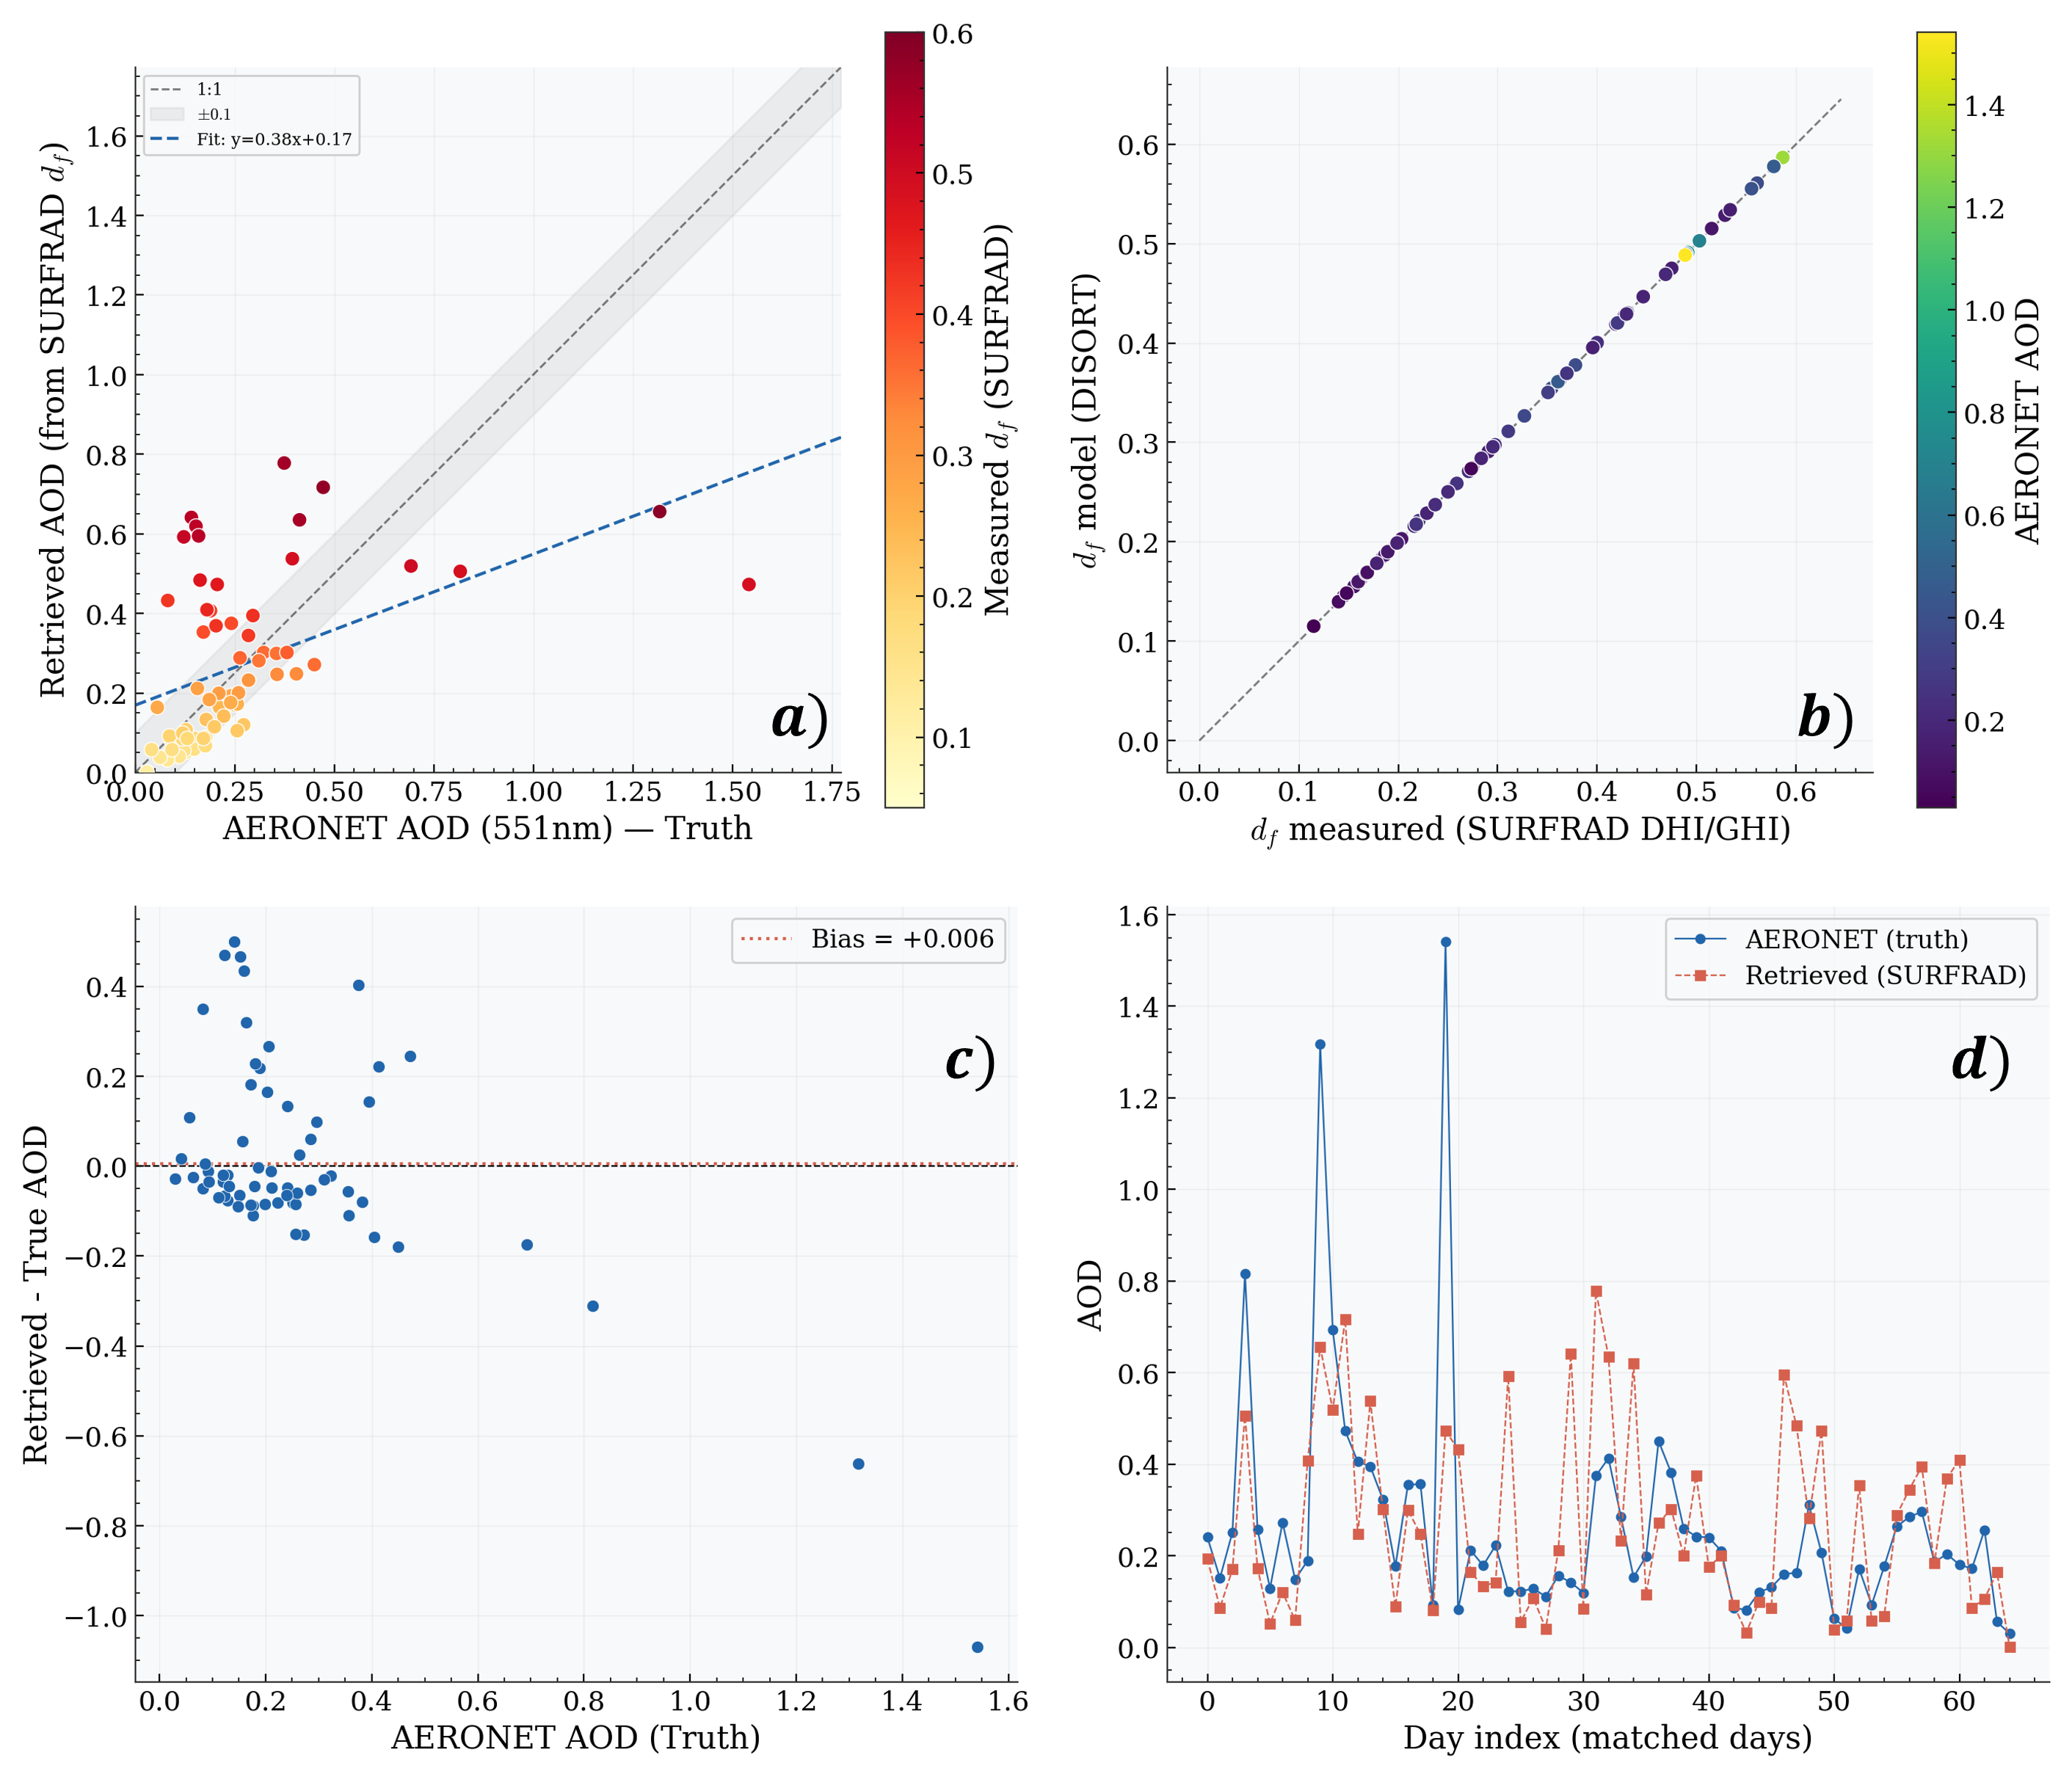
\includegraphics[width=0.6\textwidth]{Images_final_report/Level3_AERONET_retrieval_N36_theta030.png}
	\caption{Real-data AOD retrieval from SURFRAD surface radiation measurements, validated against AERONET direct-sun AOD at 550~nm (Bondville site, 65 matched days).
	$N=36$ streams, $\theta_0=30^{\circ}$.
	(a)~Retrieved AOD vs AERONET truth, colour-coded by measured diffuse fraction $d_f$ (see Section~\ref{sec:methods});
	(b)~Modelled vs measured diffuse fraction ($d_f = \mathrm{DHI/GHI}$), showing good agreement along the 1:1 line.
	(c)~Retrieval error (retrieved $-$ true) vs AERONET AOD; bias~$=+0.006$.
	(d)~Time series of AERONET (blue) and SURFRAD-retrieved (red) AOD over the 65 matched days.}
	\label{fig:level3_retrieval}
\end{figure}

Figure~\ref{fig:level3_retrieval} presents the real-data AOD retrieval
via diffuse fraction matching.  The overall bias is $+0.006$
(panel~c), indicating that the model is essentially unbiased on
average.  However, panel~(a) reveals a critical limitation: for
AERONET AOD $\gtrsim 0.3$, the retrieved AOD systematically
underestimates the truth, with errors exceeding $-0.5$ for the
heaviest aerosol events ($\tau > 1$).  The fit line slope ($y =
0.38x + 0.17$) deviates substantially from 1:1.  This degradation
has a clear physical origin: the diffuse fraction $d_f = \text{DHI}/\text{GHI}$
saturates at high AOD.  From the RTE perspective, as $\tau$ increases,
the direct-beam component $F_0 \mu_0 e^{-\tau/\mu_0}$ decays
exponentially while the diffuse flux grows only sub-linearly (because
multiple scattering redistributes energy but cannot create it); thus
$d_f$ approaches an asymptotic value near 1, and the bijective
relationship $d_f(\tau)$ required for the bisection inversion
(Section~\ref{sec:methods}) becomes nearly flat, dramatically
reducing sensitivity.  For the configuration used here ($\mu_0 =
\cos 30^{\circ} \approx 0.866$), the direct beam transmission
$e^{-\tau/\mu_0}$ drops below 1\% of $F_0$ at $\tau \approx 4$, and
the derivative $\partial d_f / \partial \tau \to 0$.  A small
uncertainty in the measured $d_f$ then maps into a large uncertainty
in the retrieved AOD.  Furthermore, the 1D plane-parallel assumption
neglects horizontal photon transport and 3D cloud effects that become
significant in high-AOD, turbid conditions
\cite{thomas2002}.  The colour coding in panel~(a)
confirms this interpretation: points with high measured $d_f$ (warm
colours) cluster in the high-AOD region where the retrieval fails.
Panel~(b) demonstrates that the forward model accurately reproduces
the measured diffuse fraction along the 1:1 line for $d_f < 0.4$,
validating the DISORT solver's flux calculations under moderate
aerosol conditions.

\subsection{Parameter Sensitivity Studies}

\subsubsection{Study A: Sensitivity to Single Scattering Albedo}

\begin{figure}[H]
	\centering
	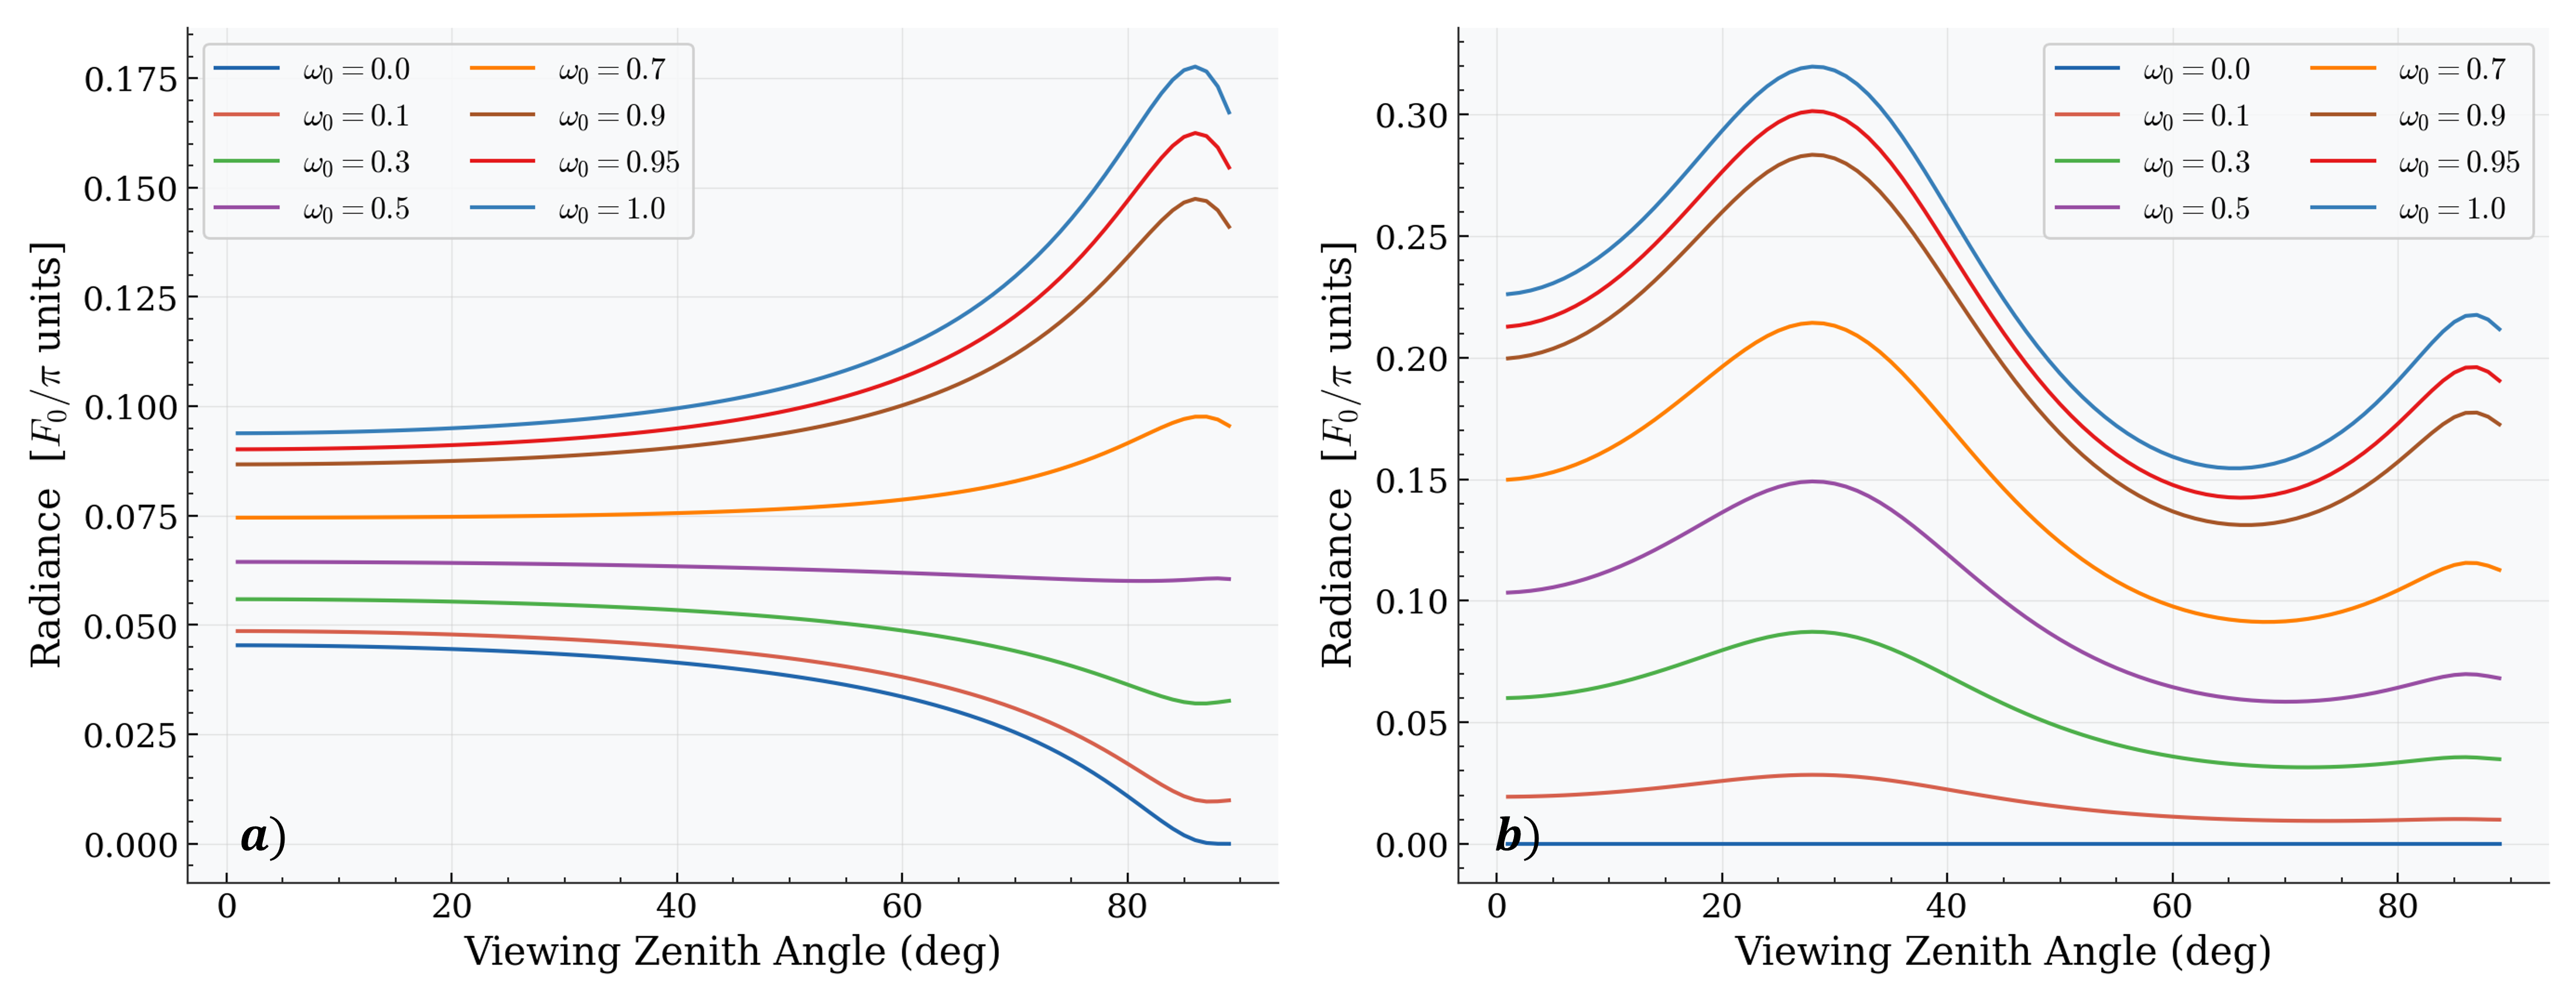
\includegraphics[width=0.7\textwidth]{Images_final_report/Study_A_SSA_sweep_AOD_03_g07_albedo_01_N36_theta030.png}
	\caption{Sensitivity to single scattering albedo $\omega_0$.
	Fixed parameters: $\tau=0.3$, $g=0.7$, $A_s=0.1$, $N=36$ streams, $\theta_0=30^{\circ}$.
	$\omega_0$ varies from 0.0 (purely absorbing) to 1.0 (conservative scattering).
	(a)~TOA upwelling radiance. (b)~BOA downwelling radiance.}
	\label{fig:study_a}
\end{figure}

Figure~\ref{fig:study_a} reveals a qualitative transition in the
angular structure as $\omega_0$ crosses approximately 0.5.  For
$\omega_0 \geq 0.5$ (dominant scattering), the radiance increases
monotonically towards the horizon at both TOA and BOA, following the
path-length saturation effect of
Eq.~\eqref{eq:horizon_saturation}: the source function
$S \propto \omega_0$ is strong enough that the growing optical path at
grazing angles produces a net gain.  For $\omega_0 < 0.5$ (dominant
absorption), the horizon enhancement weakens or disappears.
Physically, when absorption dominates, the source function $S_0$ is
small (proportional to the scattering fraction~$\omega_0$), and the
extinction along the long oblique path removes more photons than
scattering can supply.  The radiance at TOA (panel~a) for
$\omega_0 = 0$ is dominated by the surface-reflected component
$I_{\text{surf}} e^{-\tau/\mu}$, which decreases towards the horizon
because the transmission factor $e^{-\tau/\mu}$ vanishes as $\mu \to
0^+$.  At BOA (panel~b), the $\omega_0 = 0$ curve is essentially zero
because there is no scattering source and the surface reflection does
not contribute to the downwelling field.  The ordering of the curves
at any angle follows directly from the source function:
$S_0 \propto \omega_0$, so higher SSA produces proportionally more
scattered intensity.

\subsubsection{Study B: Sensitivity to Aerosol Optical Depth}

\begin{figure}[H]
	\centering
	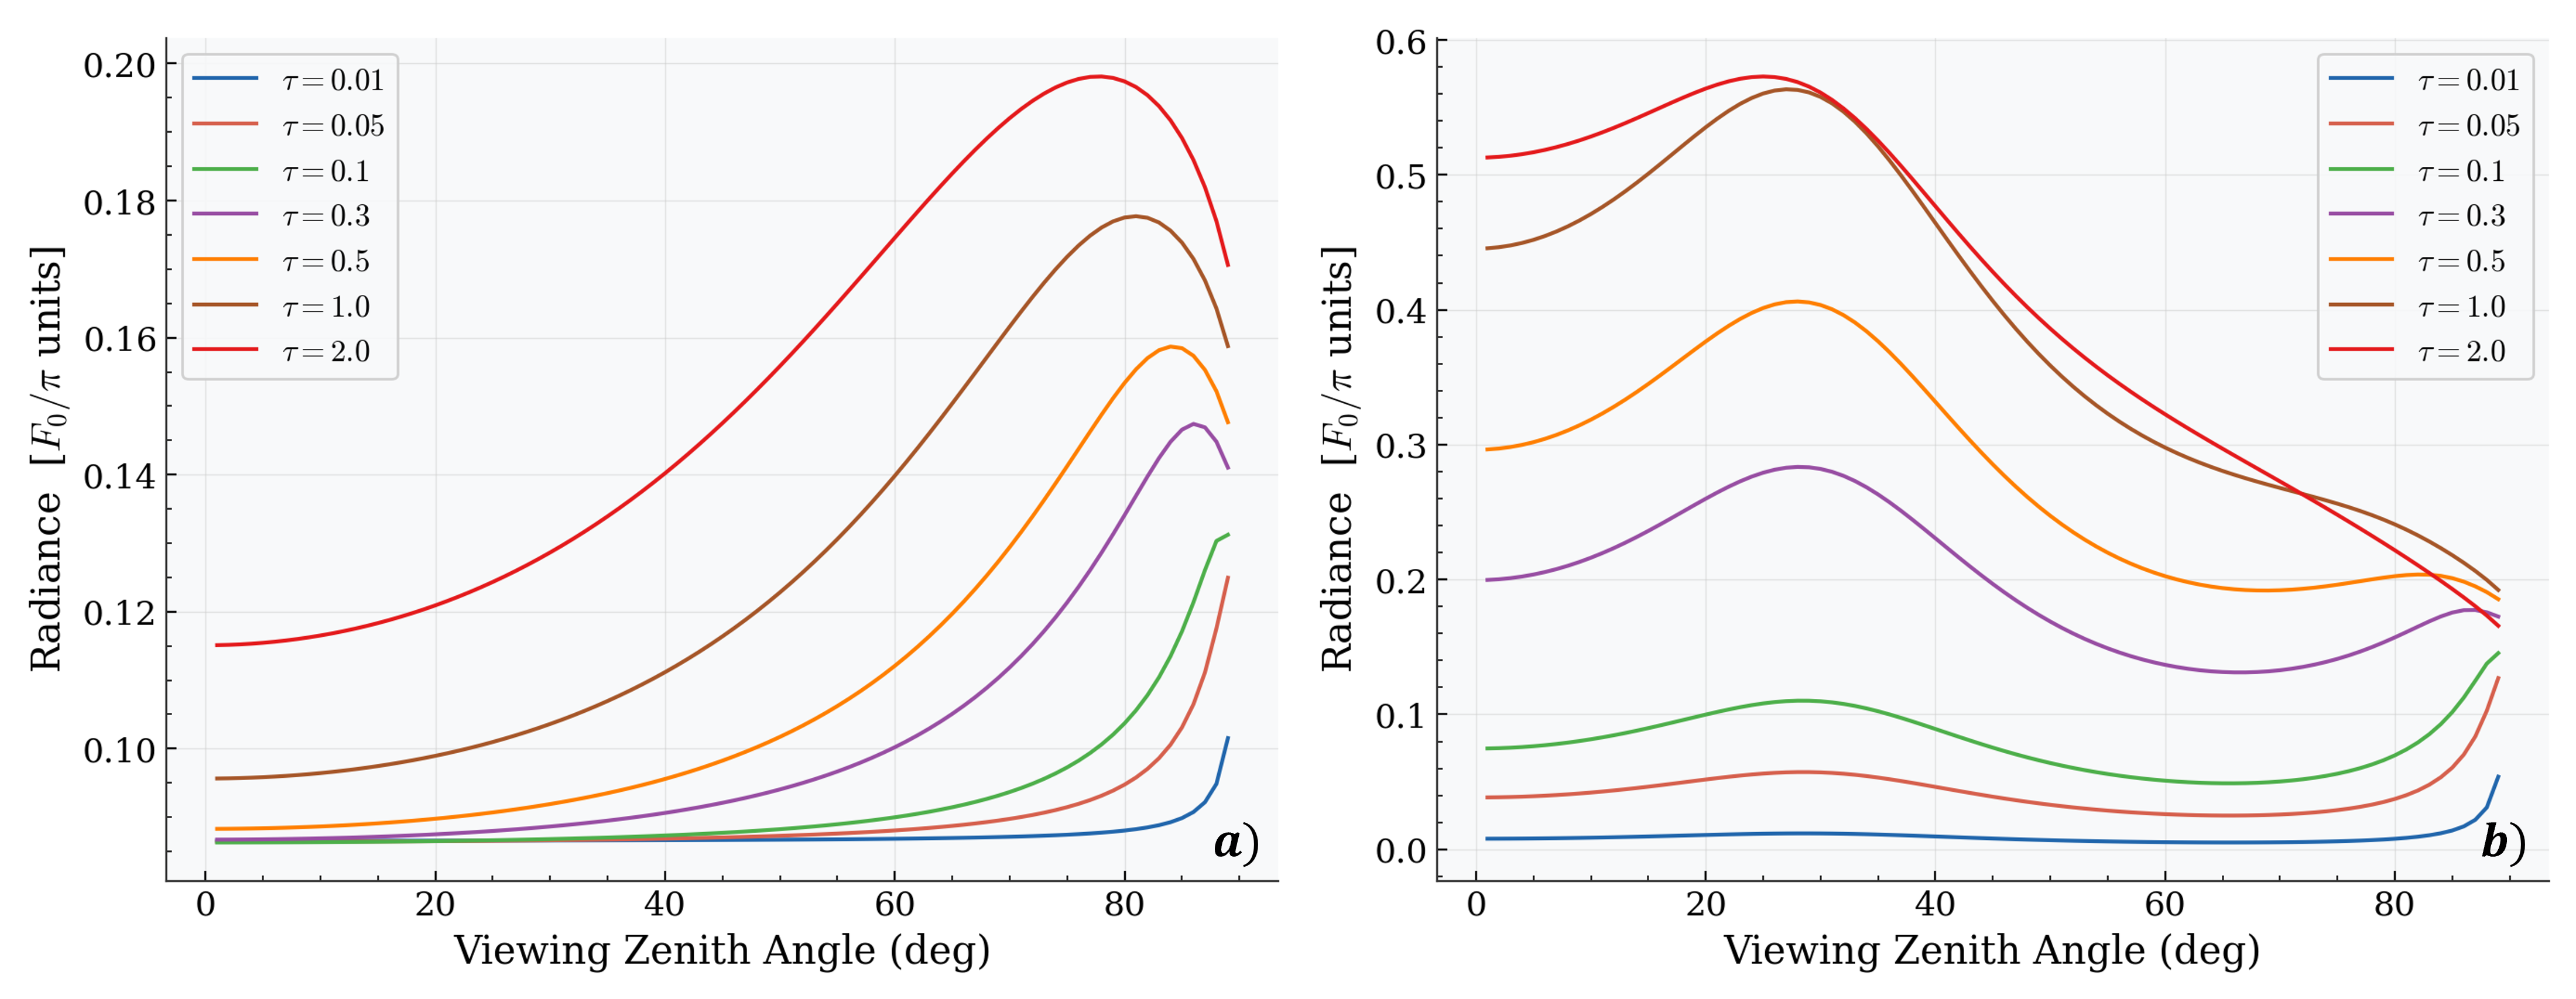
\includegraphics[width=0.7\textwidth]{Images_final_report/Study_B_AOD_sweep_SSA_09_g07_albedo_01_N36_theta030.png}
	\caption{Sensitivity to aerosol optical depth $\tau$.
	Fixed parameters: $\omega_0=0.9$, $g=0.7$, $A_s=0.1$, $N=36$ streams, $\theta_0=30^{\circ}$.
	$\tau$ varies from 0.01 to 2.0.
	(a)~TOA upwelling radiance. (b)~BOA downwelling radiance.}
	\label{fig:study_b}
\end{figure}

Figure~\ref{fig:study_b} shows that increasing $\tau$ enhances the
radiance at both TOA and BOA across all viewing angles.  The physical
mechanism is straightforward: larger $\tau$ implies more scattering
material in the column, so the source function receives more
contributions from the solar beam at each layer.  From the formal
solution, the scattered intensity scales as $I_{\text{scat}} \propto
S_0(1 - e^{-\Delta\tau/\mu})$, which grows with $\Delta\tau$ at
every angle.  At TOA (panel~a), all curves converge to relatively
low values at nadir ($\theta_v = 0^{\circ}$, $\mu = 1$) because
the short vertical path limits the scattering contribution, while the
horizon enhancement is amplified by larger $\tau$ because the
saturation value~$S_0$ itself increases with the amount of scattering
material.  At BOA (panel~b), the forward-scattering peak near
$\theta_v \approx 30^{\circ}$ (the solar aureole) grows dramatically
with $\tau$: for $\tau = 2.0$, the forward peak reaches ${\sim}0.55$
$F_0/\pi$ units, compared to ${\sim}0.02$ for $\tau = 0.01$.  This
peak arises from the phase function $p(-\mu, -\mu_0)$ being maximum
when the viewing direction approaches the solar beam direction, and
its magnitude scales with the total scattering optical depth
$\tau \omega_0$.

\subsubsection{Study C: Sensitivity to Asymmetry Parameter}

\begin{figure}[H]
	\centering
	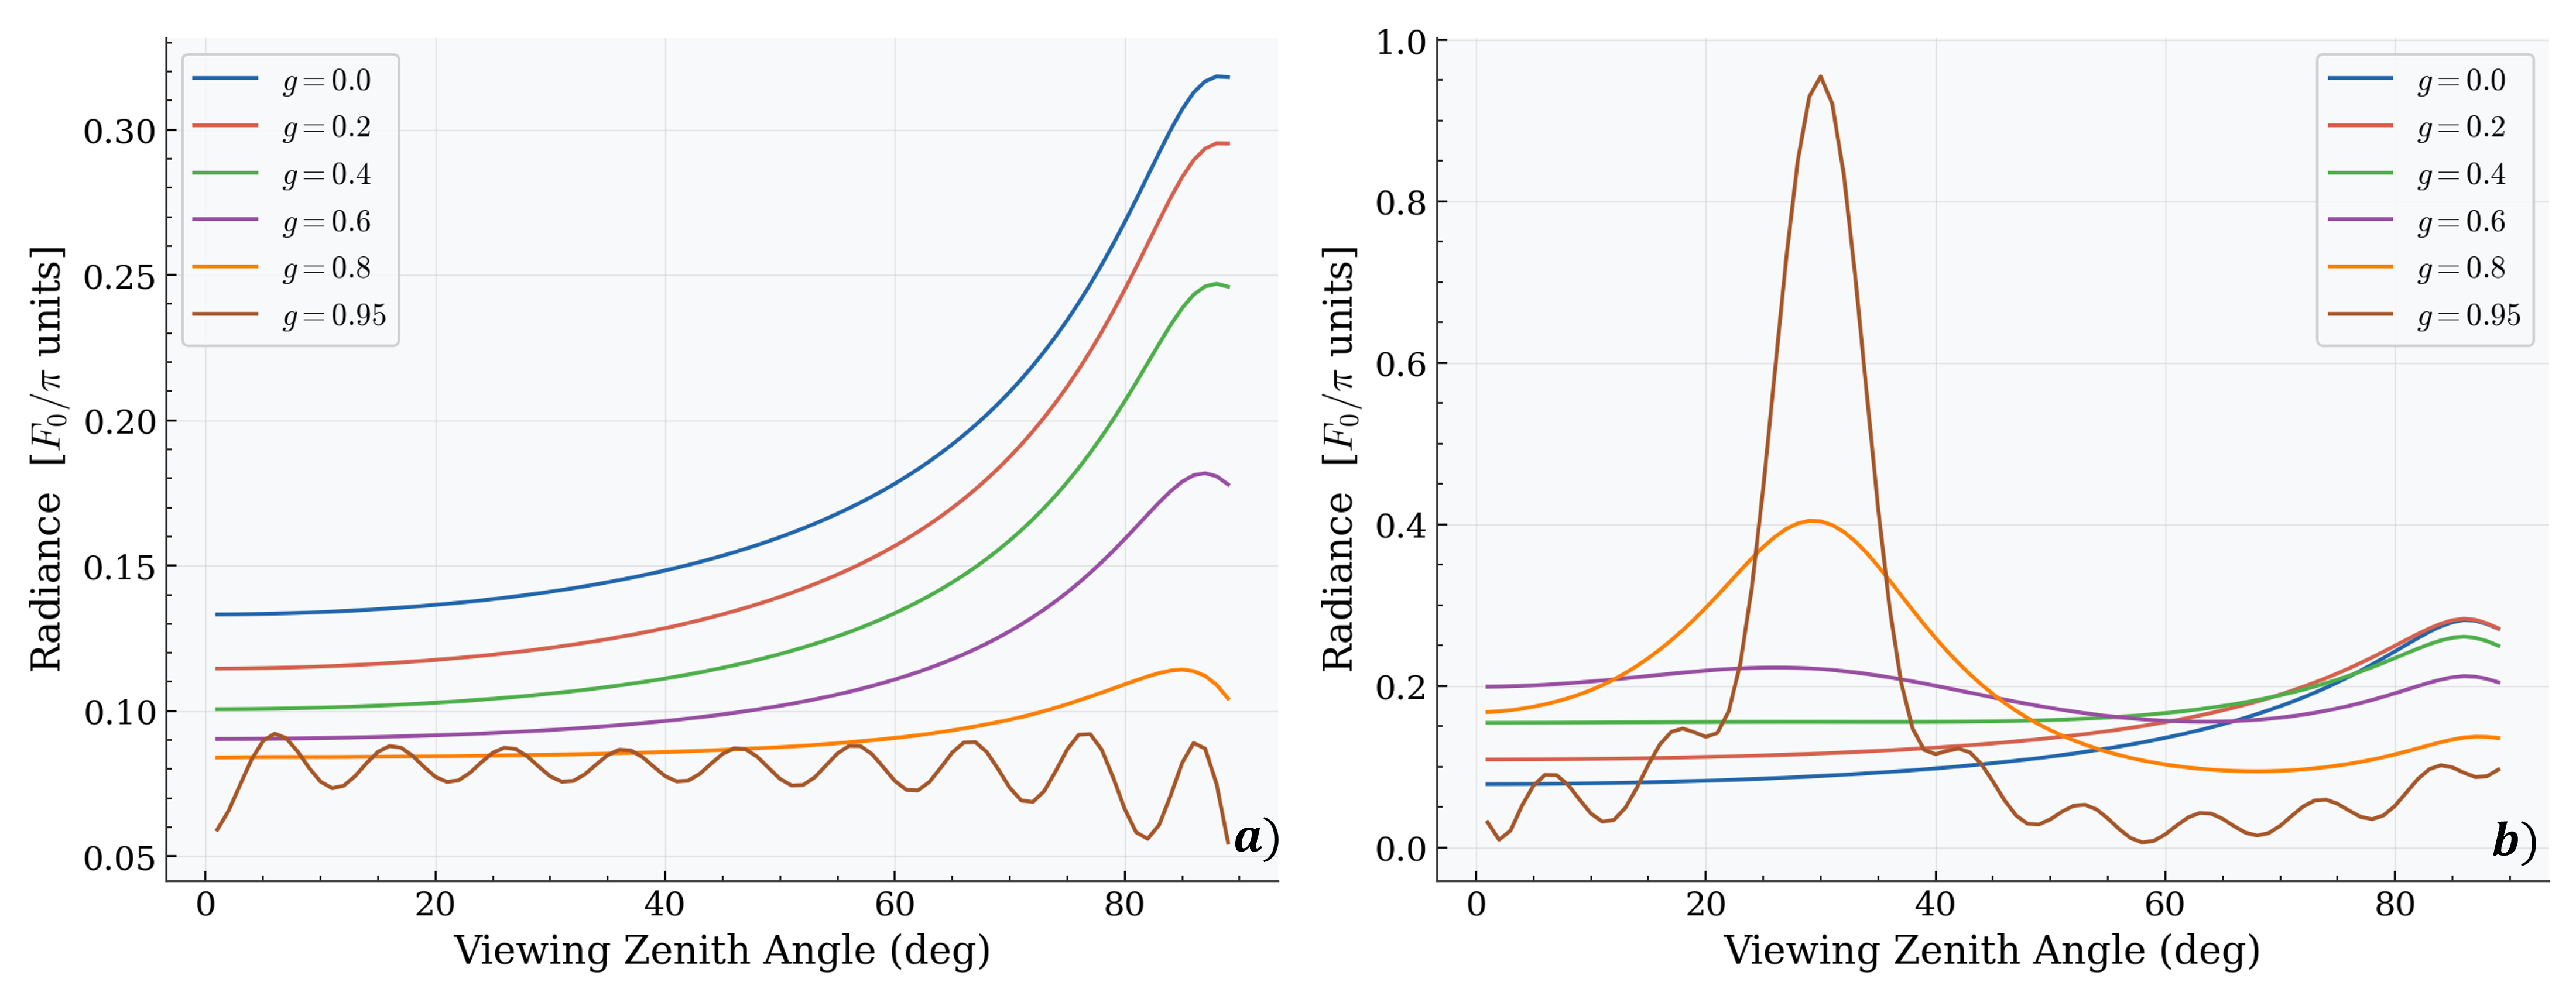
\includegraphics[width=0.7\textwidth]{Images_final_report/Study_C_g_sweep_AOD_03_SSA_09_albedo_01_N36_theta030.png}
	\caption{Sensitivity to asymmetry parameter $g$.
	Fixed parameters: $\tau=0.3$, $\omega_0=0.9$, $A_s=0.1$, $N=36$ streams, $\theta_0=30^{\circ}$.
	$g$ varies from 0.0 (isotropic) to 0.95 (strongly forward-peaked).
	(a)~TOA upwelling radiance. (b)~BOA downwelling radiance.}
	\label{fig:study_c}
\end{figure}

Figure~\ref{fig:study_c} demonstrates the strong and non-trivial
effect of the asymmetry parameter.  At TOA (panel~a), increasing $g$
from 0 to 0.8 \emph{decreases} the upwelling radiance at all angles.
This is physically expected: a larger $g$ redirects more of the
scattered energy into the forward hemisphere (downward), reducing
the fraction available for backscattering towards the TOA observer.
Quantitatively, for the Henyey--Greenstein phase function
(Eq.~\ref{eq:phase_azimuthal}), the backscatter fraction at
$\cos\Theta = -1$ is $p(-1) = (1 - g^2)/(1 + g)^3$, which decreases
from 1 (at $g = 0$) to 0.0256 (at $g = 0.8$).  At BOA (panel~b), the
opposite occurs: increasing $g$ concentrates the scattered radiation
into a narrow forward peak centred at $\theta_v \approx \theta_0 =
30^{\circ}$ (the solar aureole).  For $g = 0.8$, this peak reaches
${\sim}0.95$ $F_0/\pi$ units---nearly five times the isotropic value.

The $g = 0.95$ curve exhibits pronounced numerical oscillations at
both TOA and BOA.  This is a direct consequence of the Legendre
truncation: the HG phase function is expanded as $p(\cos\Theta) =
\sum_{l=0}^{N-1} (2l+1)\,g^l\,P_l(\cos\Theta)$
(Eq.~\ref{eq:phase_azimuthal}), and the last retained coefficient is
$\chi_{N-1} = g^{N-1}$.  For $N = 36$ and $g = 0.95$,
$\chi_{35} = (2 \times 35 + 1) \times 0.95^{35} = 71 \times 0.166 =
11.8$, which is far from negligible, indicating that the truncation
cuts off a significant portion of the phase function's energy.  The
resulting Gibbs-like oscillations propagate into the radiance field
through the source function~$S(\tau, \mu)$
(Eq.~\ref{eq:formal_up}).  This numerical artefact is analysed in
detail in Section~\ref{sec:legendre_truncation} and
Appendix~\ref{app:figures}.

\subsubsection{Study D: Sensitivity to Surface Albedo}

\begin{figure}[H]
	\centering
	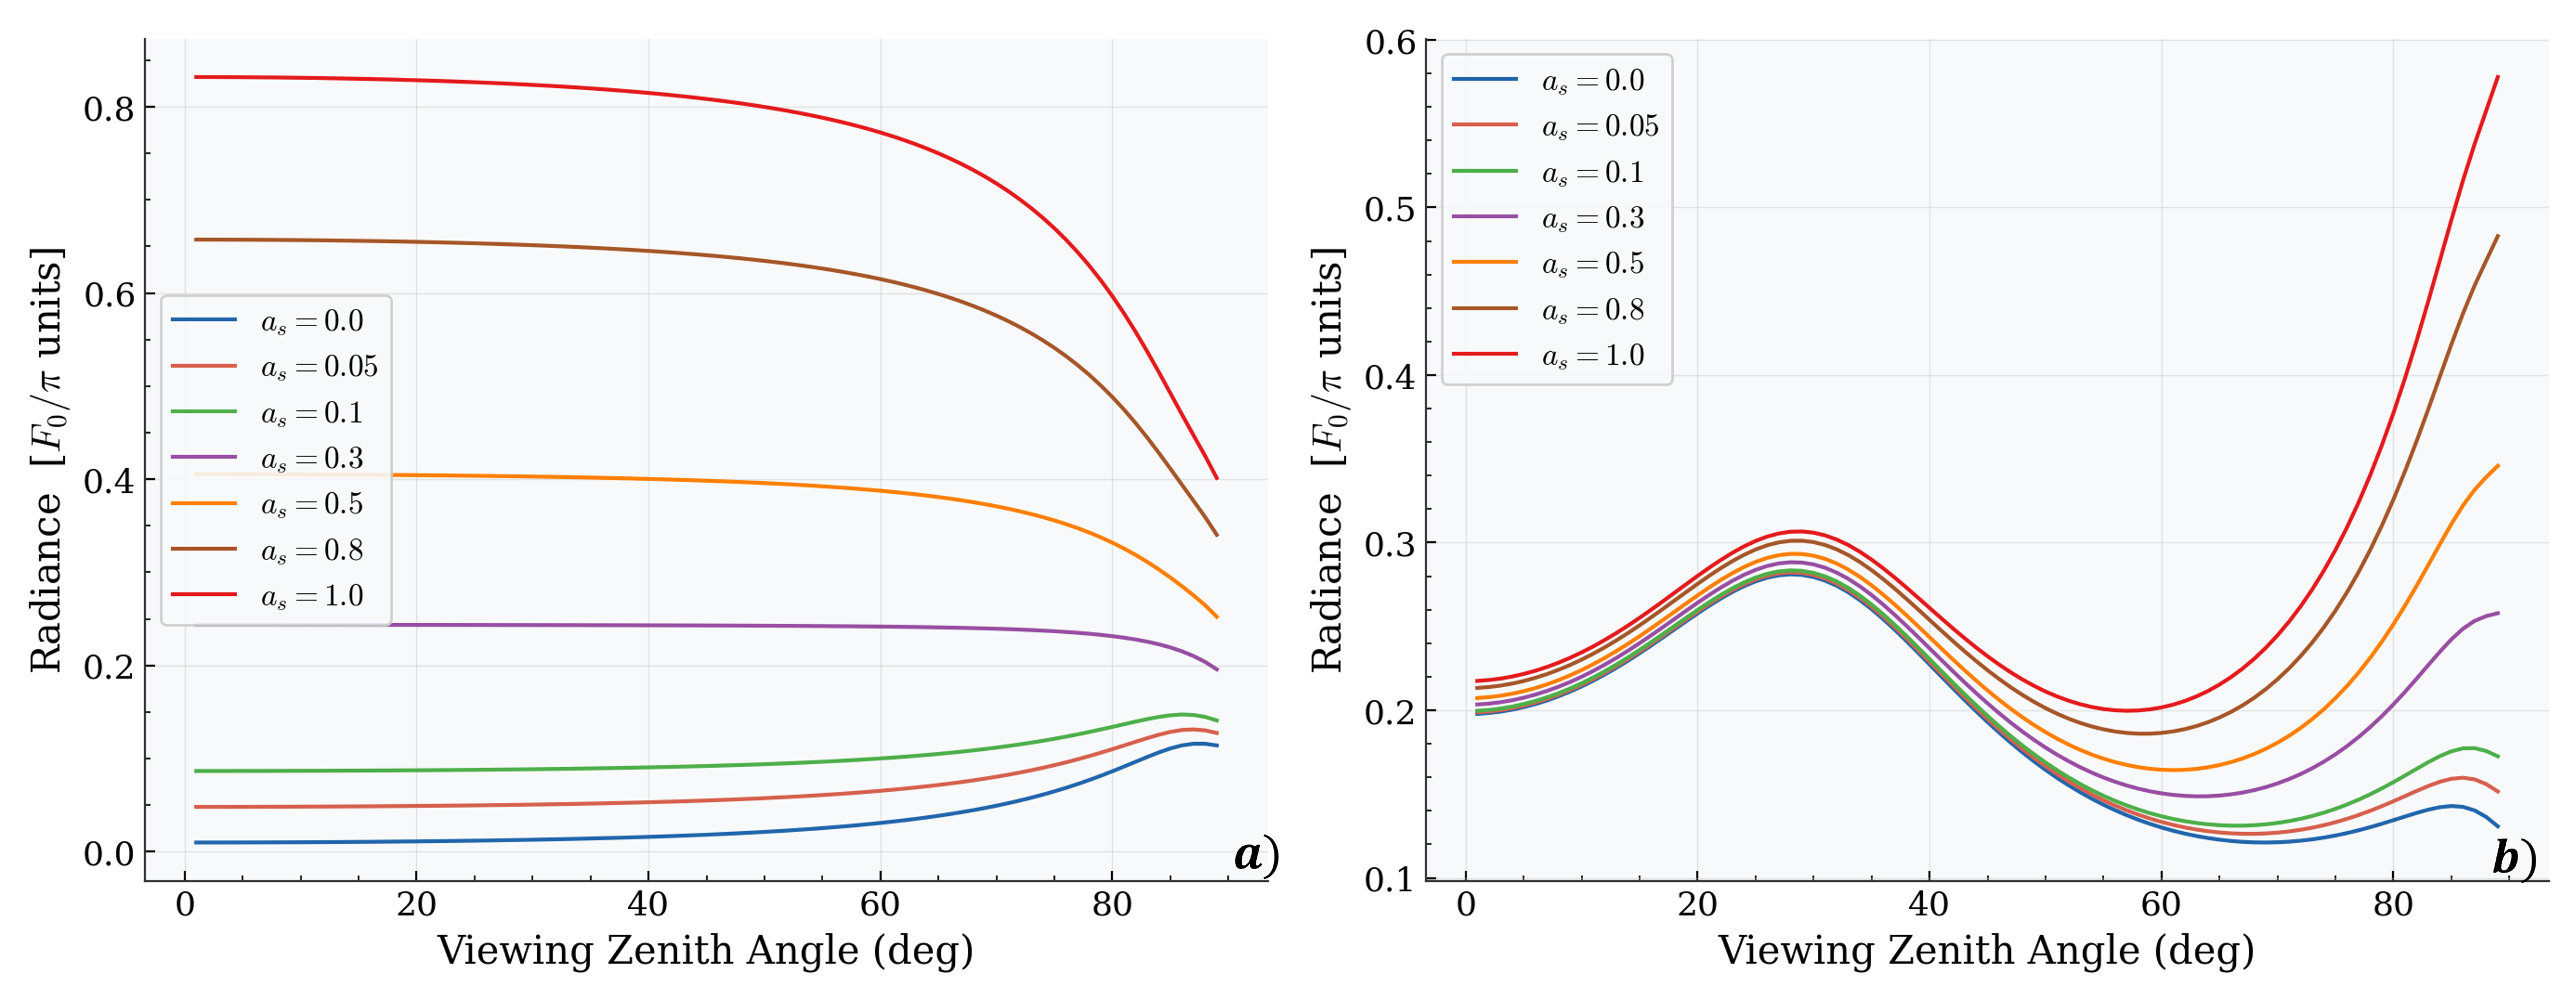
\includegraphics[width=0.7\textwidth]{Images_final_report/Study_D_albedo_sweep_AOD_03_SSA_09_g07_N36_theta030.png}
	\caption{Sensitivity to surface albedo $A_s$.
	Fixed parameters: $\tau=0.3$, $\omega_0=0.9$, $g=0.7$, $N=36$ streams, $\theta_0=30^{\circ}$.
	$A_s$ varies from 0.0 (black surface) to 1.0 (perfect reflector).
	(a)~TOA upwelling radiance. (b)~BOA downwelling radiance.}
	\label{fig:study_d}
\end{figure}

Figure~\ref{fig:study_d} shows that increasing the surface albedo
$A_s$ elevates the TOA radiance (panel~a) uniformly across all
viewing angles.  The mechanism follows from the lower boundary
condition (Eq.~\ref{eq:bc_boa}): a higher $A_s$ reflects more of the
downwelling flux isotropically into the upward hemisphere, producing a
surface-reflected component $I_{\text{surf}} \propto A_s$ that is
transmitted to the TOA observer after attenuation by the factor
$e^{-\tau/\mu}$.  For nearly transparent atmospheres ($\tau = 0.3$),
this surface contribution dominates: at nadir ($\mu = 1$), the
transmission $e^{-0.3} \approx 0.74$ is high, and the TOA intensity
is nearly proportional to $A_s$.  At BOA (panel~b), the effect of
$A_s$ is subtler: higher surface albedo enhances the downwelling
radiance through multiple reflections between the surface and the
atmosphere (the trapping effect), but the sensitivity is weaker
because the primary BOA signal comes from atmospheric scattering of
the direct beam.

\subsubsection{Study E: Sensitivity to Solar Zenith Angle}

\begin{figure}[H]
	\centering
	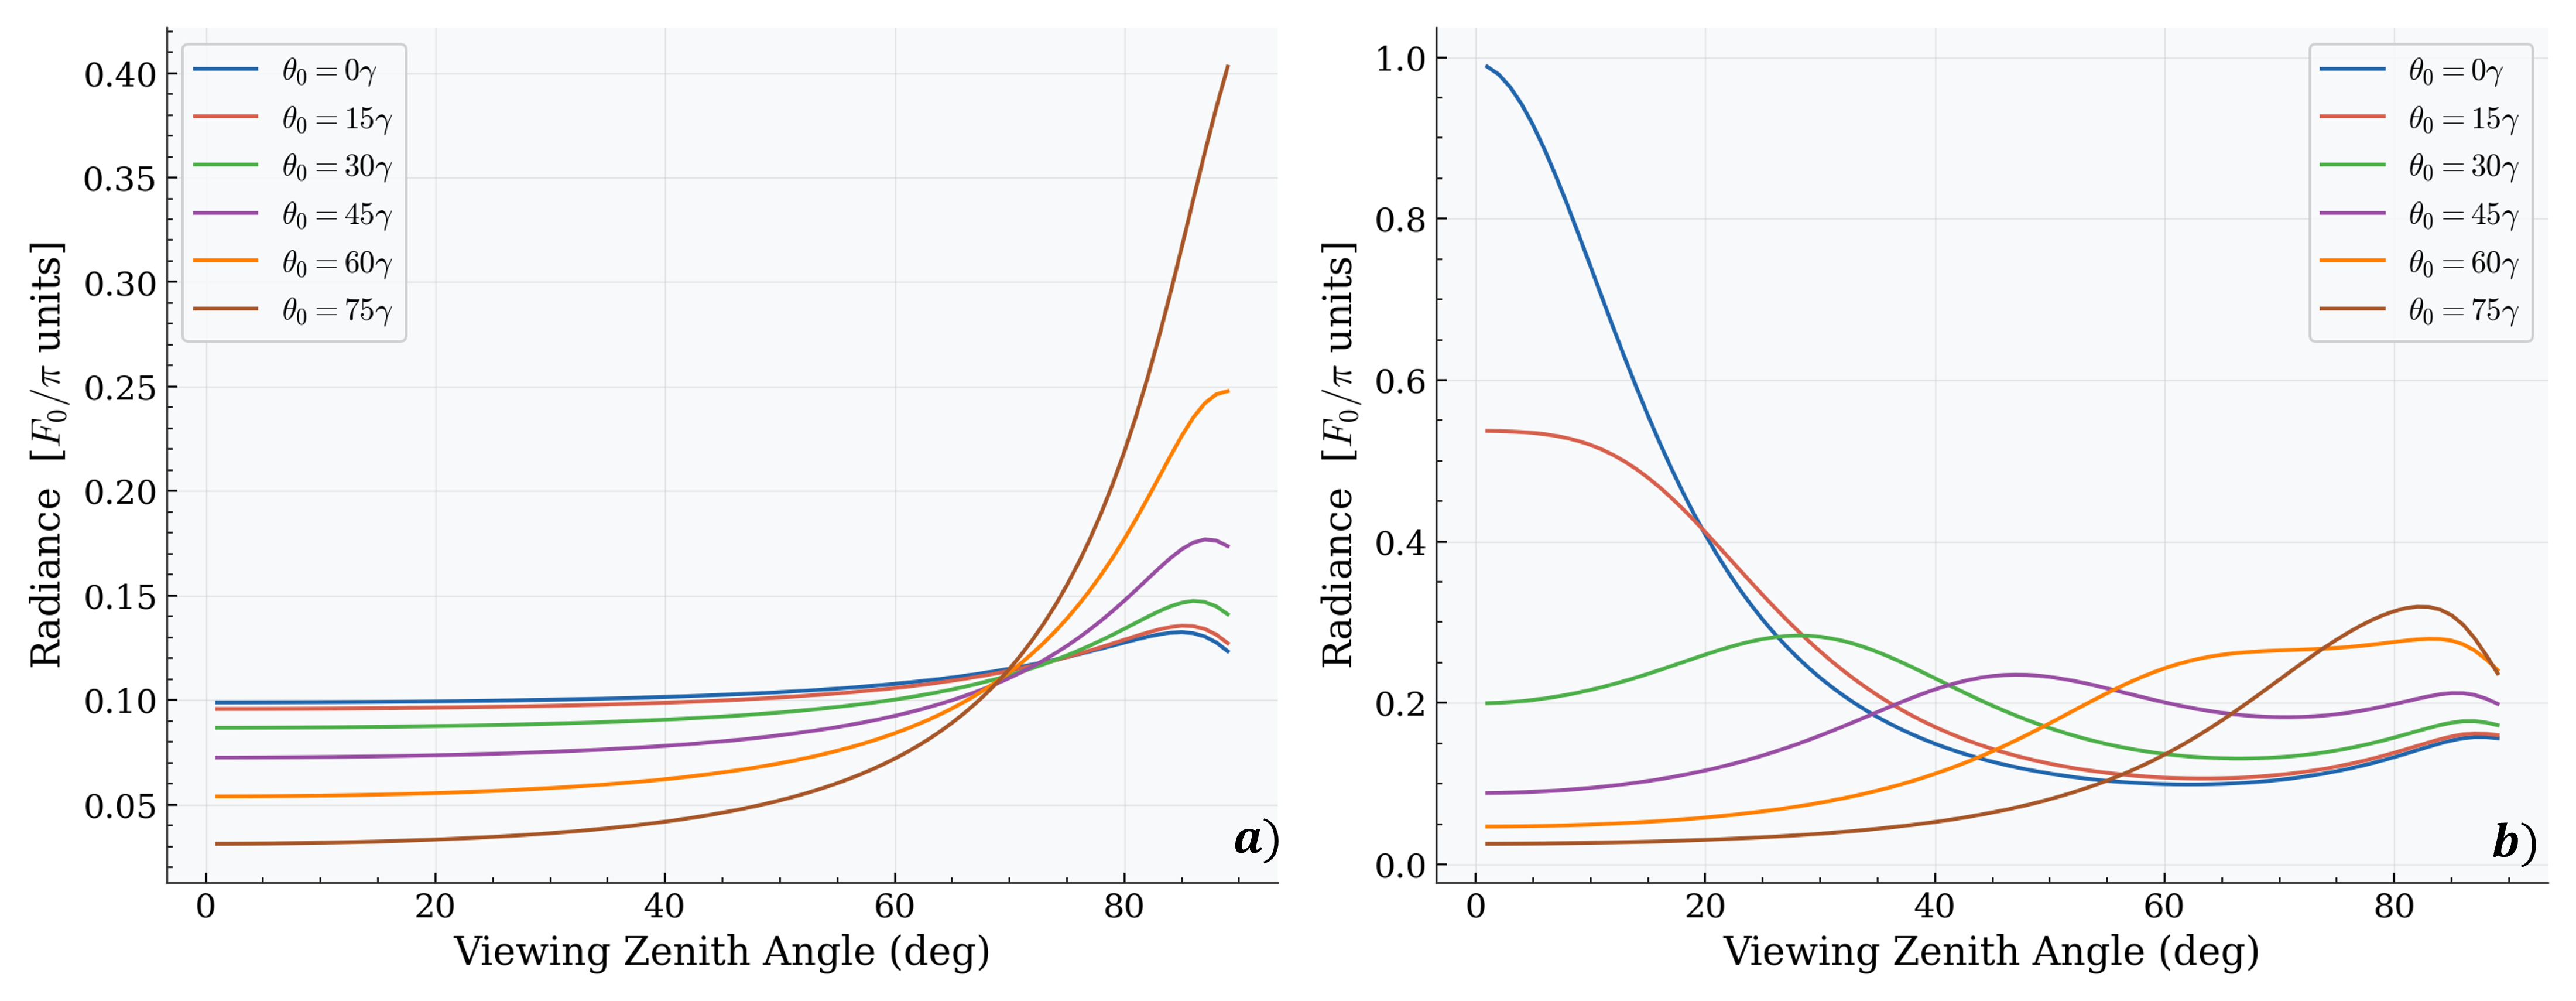
\includegraphics[width=0.7\textwidth]{Images_final_report/Study_E_SZA_sweep_AOD_03_SSA_09_g07_albedo_01_N36.png}
	\caption{Sensitivity to solar zenith angle $\theta_0$.
	Fixed parameters: $\tau=0.3$, $\omega_0=0.9$, $g=0.7$, $A_s=0.1$, $N=36$ streams.
	$\theta_0$ varies from $0^{\circ}$ (overhead sun) to $75^{\circ}$ (low sun).
	(a)~TOA upwelling radiance. (b)~BOA downwelling radiance.}
	\label{fig:study_e}
\end{figure}

Figure~\ref{fig:study_e} reveals a particularly instructive angular
pattern.  At BOA (panel~b), the forward-scattering peak shifts from
$\theta_v = 0^{\circ}$ (for $\theta_0 = 0^{\circ}$, overhead sun) to
$\theta_v \approx 75^{\circ}$ (for $\theta_0 = 75^{\circ}$, low sun),
tracking the solar direction as expected from the phase function
$p(-\mu, -\mu_0)$, which peaks when $\mu \approx \mu_0$ (viewing
along the solar beam).  For low sun ($\theta_0 = 75^{\circ}$), the
forward peak merges with the horizon enhancement, producing the
largest BOA radiance.  The BOA peak at $\theta_0 = 0^{\circ}$ is the
tallest (${\sim}1.0$ $F_0/\pi$ units) because overhead illumination
concentrates the aureole into the narrowest angular range.

At TOA (panel~a), the pattern is more nuanced.  For high sun
($\theta_0 \leq 30^{\circ}$), the radiance is relatively flat and
low because the solar beam traverses a short atmospheric path
($\tau/\mu_0$ is small), producing modest scattering.  For low sun
($\theta_0 = 60^{\circ}$--$75^{\circ}$), the beam source term
$Q \propto e^{-\tau/\mu_0}$ is attenuated more strongly, but the
longer slant path increases the effective scattering volume; the
dominant effect near the horizon is again the path-length saturation
of Eq.~\eqref{eq:horizon_saturation}.

\subsubsection{Study F: Realistic Atmospheric Scenarios}

\begin{figure}[H]
	\centering
	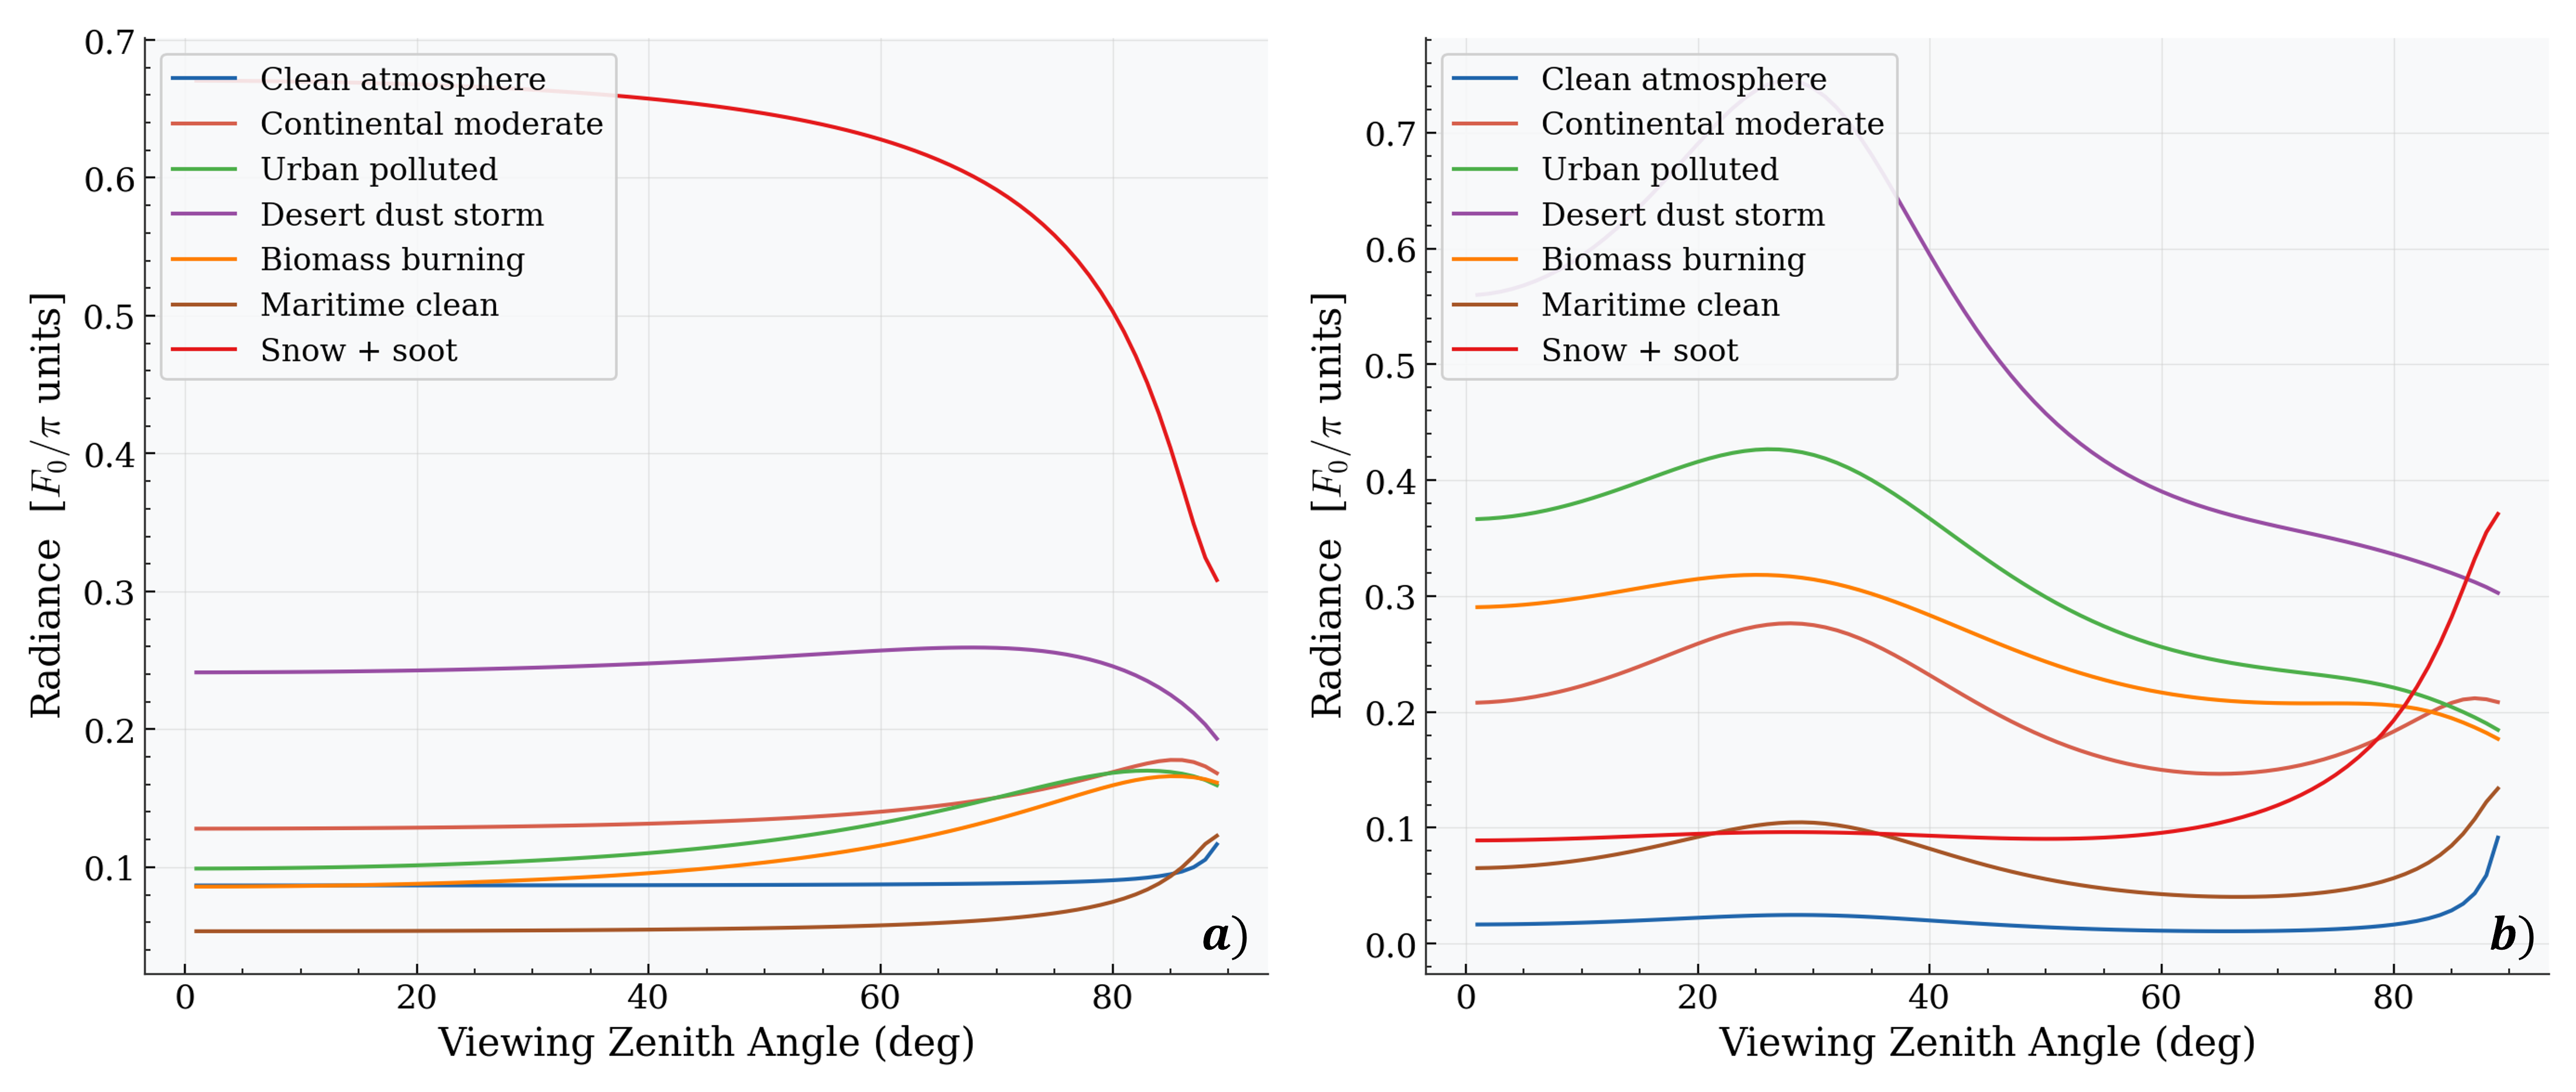
\includegraphics[width=0.7\textwidth]{Images_final_report/Study_F_scenarios_N36_theta030.png}
	\caption{Radiance fields for seven realistic atmospheric scenarios ($N=36$ streams, $\theta_0=30^{\circ}$).
		(a)~TOA upwelling radiance. (b)~BOA downwelling radiance.}
	\label{fig:study_f}
\end{figure}

Figure~\ref{fig:study_f} synthesises the individual parameter
sensitivities by comparing seven scenarios that span the diversity of
real atmospheric conditions.  At TOA (panel~a), the snow+soot scenario
($\tau = 0.15$, $\omega_0 = 0.70$, $A_s = 0.85$) produces the highest
radiance despite having a low AOD, because its very high surface
albedo dominates the upwelling signal; the radiance decreases towards
the horizon because the surface-reflected component is attenuated by
$e^{-\tau/\mu}$ (same effect as the extreme case in
Figure~\ref{fig:extreme_cases}d).  The desert dust storm ($\tau =
1.50$) generates the second-largest TOA radiance, driven by its high
optical depth.  At BOA (panel~b), the desert dust storm shows the
strongest forward-scattering peak ($\theta_v \approx 30^{\circ}$),
consistent with its large $\tau$ and $g$; the clean and maritime
scenarios produce minimal downwelling radiance, as expected for their
low optical depths ($\tau \leq 0.08$).

\subsection{Legendre Truncation and Stream Convergence}
\label{sec:legendre_truncation}

The numerical oscillations observed for $g = 0.95$ in
Figure~\ref{fig:study_c} originate from the finite Legendre expansion
of the phase function.  The Henyey--Greenstein phase function has
Legendre coefficients $\chi_l = g^l$
(Eq.~\ref{eq:phase_azimuthal}), so the expansion converges only when
$(2l+1)\,g^l \to 0$ for $l \to N$.  For $g = 0.7$ and $N = 36$, the
last coefficient is $(2 \times 35 + 1) \times 0.7^{35} = 71 \times
3.2 \times 10^{-6} \approx 2.3 \times 10^{-4}$, which is negligible:
the truncation is effectively exact, and
Figure~\ref{fig:legendre_truncation}(a) confirms that all truncation
orders ($N = 16$, 36, 64, 80) overlap with the exact HG curve.  For
$g = 0.9$, $\chi_{35} = 71 \times 0.9^{35} = 71 \times 0.025 = 1.8$,
and clear Gibbs oscillations appear for $N = 16$ while $N \geq 36$
still provides an acceptable approximation
(Figure~\ref{fig:legendre_truncation}b).  For $g = 0.95$,
$\chi_{35} = 71 \times 0.166 = 11.8$: truncation at $N = 36$ retains
less than half of the phase function energy, and even $N = 80$
($\chi_{79} = 159 \times 0.95^{79} = 159 \times 0.017 = 2.7$)
exhibits residual oscillations
(Figure~\ref{fig:legendre_truncation}c).

The delta-M method (Eq.~\ref{eq:deltam_decomp}) mitigates this
problem by extracting the forward-scattering peak into a delta
function and solving the RTE with rescaled optical properties
(Eq.~\ref{eq:deltam_scaling}).  Figure~\ref{fig:g095_streams}
compares the solution with delta-M ON (left column) and OFF (right
column) for $g = 0.95$ at different stream counts.  Without delta-M
(panels~b, d), even $N = 128$ streams produce visible oscillations at
TOA, because the unscaled asymmetry parameter $g = 0.95$ requires
$l > 130$ Legendre terms for convergence.  With delta-M ON (panels~a,
c), the rescaled asymmetry parameter $g^* = (g - f)/(1 - f)$ is
substantially reduced (for $N = 36$, $f = g^{36} = 0.95^{36} = 0.16$,
giving $g^* = (0.95 - 0.16)/(1 - 0.16) = 0.94$; for $N = 64$,
$f = 0.95^{64} = 0.037$, $g^* = 0.95$; for $N = 128$,
$f = 0.95^{128} = 0.0013$, $g^* = 0.950$), but the crucial effect is
that the rescaled phase function $p'(\cos\Theta)$ has its sharp peak
removed, so $N = 64$ streams with delta-M ON already provide a smooth
and converged solution.  At BOA (panels~c, d), the forward-scattering
peak near $\theta_v \approx 30^{\circ}$ converges much faster because
the source-function integration naturally captures the forward lobe
through the phase function $p(-\mu, -\mu_0)$ evaluated at the solar
direction.


% ====================================================================
\section{Uncertainty Analysis}
\label{sec:uncertainty}
% ====================================================================

The uncertainty budget comprises forward-model errors, noise propagation, and regularisation bias.

The DISORT solver introduces two controllable approximations.  The Legendre truncation at order~$N$ produces negligible error for $g = 0.7$ ($\chi_{35} \sim 10^{-4}$) but causes 5--10\% radiance oscillations for $g = 0.95$ ($\chi_{35} \approx 11.8$); the delta-M method reduces this below 1\% for $N \geq 64$ (Figure~\ref{fig:g095_streams}).  The source-function interpolation reproduces the discrete solution at quadrature nodes with machine precision, with inter-node errors of $O(1/N^2)$.  The 1D plane-parallel geometry is adequate for uniform cloud-free conditions but becomes a dominant error source in turbid, heterogeneous scenes \cite{thomas2002}.

The sensitivity studies (Figures~\ref{fig:study_a}--\ref{fig:study_e}) show that the TOA radiance is most sensitive to $\omega_0$ and $A_s$, moderately to $\tau$, and weakly to~$g$, implying that $g$~retrievals are inherently noisier.  The OE posterior covariance $\hat{\mathbf{S}} = (\mathbf{K}^T \mathbf{S}_\epsilon^{-1} \mathbf{K} + \mathbf{S}_a^{-1})^{-1}$ \cite{rodgers2000} formalises this hierarchy.

The dominant retrieval uncertainty is systematic regularisation bias, not random noise.  The scalar Tikhonov penalty yields a 52\% AOD error in the 20-layer case by pulling the solution towards the a~priori regardless of data content, whereas OE reduces this to 4.3\% by weighting the constraint through $\mathbf{S}_a^{-1}$ (Figures~\ref{fig:level1_aod} and~\ref{fig:level2_lm_vs_oe}).

For the Level~3 real-data retrieval, the primary uncertainty is the saturation of $d_f(\tau)$ at high AOD: for $\tau \lesssim 0.3$ the inversion is stable (bias $\sim +0.006$), but beyond this threshold a 1\% uncertainty in $d_f$ maps into AOD errors exceeding 0.1.  Additional sources include the fixed aerosol type, fixed $\theta_0 = 30^{\circ}$, and omission of gaseous absorption.

% ====================================================================
\section{Conclusions}
\label{sec:conclusions}
% ====================================================================

A complete forward--inverse modelling chain for aerosol optical property retrieval based on the Discrete Ordinates radiative transfer method was developed and validated.  The main findings are summarised below.

\textbf{Forward model.}  The multi-layer DISORT solver satisfies energy conservation to machine precision (Figure~\ref{fig:energy_tests}), reproduces analytical limiting cases (Figure~\ref{fig:extreme_cases}), and provides continuous angular radiance fields via source-function interpolation that agree with the discrete solution at quadrature nodes (Figure~\ref{fig:discrete_vs_continuous}), confirming the correctness of the eigenvalue formulation and stabilisation scheme.

\textbf{Inverse method comparison.}  Optimal Estimation consistently outperforms LM+Tikhonov.  In the 20-layer joint retrieval, OE achieves errors below 5\% for all parameters ($\tau$: 4.3\%, $\omega_0$: 1.4\%, $g$: 3.1\%), while Tikhonov exceeds 50\% in AOD and~$g$ due to its inability to resolve the $\tau$--$g$ degeneracy (Figure~\ref{fig:level2_lm_vs_oe}).  The vertical profile reconstruction confirms that OE preserves the exponential decrease of aerosol loading with altitude (Figure~\ref{fig:level2_vertical}).

\textbf{Real-data retrieval.}  Application to 65 matched SURFRAD/AERONET days demonstrates an unbiased retrieval (bias $= +0.006$) for $\tau \lesssim 0.3$, with degradation at higher AOD driven by $d_f(\tau)$ saturation (Figure~\ref{fig:level3_retrieval}).  The underlying reason is that at high AOD the direct beam $F_0\mu_0 e^{-\tau/\mu_0}$ is nearly extinguished, so almost all surface irradiance is diffuse and $d_f \to 1$ regardless of further increases in~$\tau$; the inversion then loses its single degree of freedom.  This limitation motivates multi-angular or multi-spectral retrieval approaches.

\textbf{Parameter sensitivities and numerical convergence.}  The radiance field is most sensitive to $\omega_0$ and $A_s$, moderately to $\tau$, and weakly to~$g$ except through the BOA forward-scattering peak (Figures~\ref{fig:study_a}--\ref{fig:study_f}).  For strongly forward-scattering aerosols ($g > 0.9$), the delta-M method suppresses Legendre truncation oscillations and achieves convergence with $N = 64$ streams (Figure~\ref{fig:g095_streams}), while $N = 36$ suffices for $g \leq 0.8$.

The principal limitations are the 1D plane-parallel geometry and the assumption of a single aerosol type.  Future work could incorporate multi-spectral measurements to break the $\tau$--$g$ degeneracy, couple the solver with a size-distribution retrieval to infer microphysical properties from the Mie kernel, and assimilate multi-angular observations to improve vertical profile resolution.

% ====================================================================
%                        BIBLIOGRAPHY
% ====================================================================
\newpage
\bibliographystyle{unsrtnat}
% \bibliography{references}  % Uncomment when you have a references.bib file

% Manual references (remove when using .bib):
\begin{thebibliography}{99}

  \bibitem{ipcc2021}
    IPCC,
    \textit{Climate Change 2021: The Physical Science Basis.
    Contribution of Working Group~I to the Sixth Assessment Report}.
    Cambridge University Press, 2021.

  \bibitem{kaufman2002}
    Y.~J.~Kaufman, D.~Tanr\'e, and O.~Boucher,
    ``A satellite view of aerosols in the climate system,''
    \textit{Nature}, vol.~419, pp.~215--223, 2002.

  \bibitem{seinfeld2016}
    J.~H.~Seinfeld and S.~N.~Pandis,
    \textit{Atmospheric Chemistry and Physics: From Air Pollution to
    Climate Change}, 3rd~ed.
    John Wiley \& Sons, 2016.

  \bibitem{rodgers2000}
    C.~D.~Rodgers,
    \textit{Inverse Methods for Atmospheric Sounding: Theory and Practice}.
    World Scientific, 2000.

  \bibitem{hadamard1902}
    J.~Hadamard,
    ``Sur les probl\`emes aux d\'eriv\'ees partielles et leur
    signification physique,''
    \textit{Princeton University Bulletin}, vol.~13, pp.~49--52, 1902.

  \bibitem{tikhonov1977}
    A.~N.~Tikhonov and V.~Y.~Arsenin,
    \textit{Solutions of Ill-Posed Problems}.
    Winston \& Sons, 1977.

  \bibitem{stamnes1988}
    K.~Stamnes, S.-C.~Tsay, W.~Wiscombe, and K.~Jayaweera,
    ``Numerically stable algorithm for discrete-ordinate-method radiative
    transfer in multiple scattering and emitting layered media,''
    \textit{Appl.\ Opt.}, vol.~27, no.~12, pp.~2502--2509, 1988.

  \bibitem{holben1998}
    B.~N.~Holben \textit{et al.},
    ``AERONET---A federated instrument network and data archive for
    aerosol characterization,''
    \textit{Remote Sens.\ Environ.}, vol.~66, pp.~1--16, 1998.

  \bibitem{chandrasekhar1950}
    S.~Chandrasekhar,
    \textit{Radiative Transfer}.
    Oxford University Press, 1950.

  \bibitem{thomas2002}
    G.~E.~Thomas and K.~Stamnes,
    \textit{Radiative Transfer in the Atmosphere and Ocean}.
    Cambridge University Press, 1999.

  \bibitem{disortreport}
    K.~Stamnes, S.-C.~Tsay, W.~Wiscombe, and I.~Laszlo,
    ``DISORT, a General-Purpose Fortran Program for
    Discrete-Ordinate-Method Radiative Transfer in Scattering and
    Emitting Layered Media: Documentation of Methodology,''
    Tech.\ rep., Dept.\ of Physics and Engineering Physics,
    Stevens Institute of Technology, Hoboken, NJ, 2000.

  \bibitem{liou2002}
    K.~N.~Liou,
    \textit{An Introduction to Atmospheric Radiation}, 2nd~ed.
    Academic Press, 2002.

  \bibitem{wiscombe1977}
    W.~J.~Wiscombe,
    ``The delta-M method: Rapid yet accurate radiative flux calculations
    for strongly asymmetric phase functions,''
    \textit{J.\ Atmos.\ Sci.}, vol.~34, pp.~1408--1422, 1977.

  \bibitem{bohren1983}
    C.~F.~Bohren and D.~R.~Huffman,
    \textit{Absorption and Scattering of Light by Small Particles}.
    John Wiley \& Sons, 1983.

  \bibitem{vandeHulst1957}
    H.~C.~van~de~Hulst,
    \textit{Light Scattering by Small Particles}.
    John Wiley \& Sons, 1957.

  \bibitem{wiscombe1980}
    W.~J.~Wiscombe,
    ``Improved Mie scattering algorithms,''
    \textit{Appl.\ Opt.}, vol.~19, no.~9, pp.~1505--1509, 1980.

  \bibitem{hess1998}
    M.~Hess, P.~Koepke, and I.~Schult,
    ``Optical properties of aerosols and clouds: The software package
    OPAC,''
    \textit{Bull.\ Amer.\ Meteor.\ Soc.}, vol.~79, pp.~831--844, 1998.

  \bibitem{bodhaine1999}
    B.~A.~Bodhaine, N.~B.~Wood, E.~G.~Dutton, and J.~R.~Slusser,
    ``On Rayleigh optical depth calculations,''
    \textit{J.\ Atmos.\ Ocean.\ Technol.}, vol.~16, pp.~1854--1861, 1999.

  \bibitem{levenberg1944}
    K.~Levenberg,
    ``A method for the solution of certain non-linear problems in least
    squares,''
    \textit{Quart.\ Appl.\ Math.}, vol.~2, pp.~164--168, 1944.

  \bibitem{marquardt1963}
    D.~W.~Marquardt,
    ``An algorithm for least-squares estimation of nonlinear parameters,''
    \textit{J.\ Soc.\ Indust.\ Appl.\ Math.}, vol.~11, no.~2,
    pp.~431--441, 1963.

  \bibitem{phillips1962}
    D.~L.~Phillips,
    ``A technique for the numerical solution of certain integral
    equations of the first kind,''
    \textit{J.\ ACM}, vol.~9, pp.~84--97, 1962.

  \bibitem{twomey1963}
    S.~Twomey,
    ``On the numerical solution of Fredholm integral equations of the
    first kind by the inversion of the linear system produced by
    quadrature,''
    \textit{J.\ ACM}, vol.~10, pp.~97--101, 1963.

  \bibitem{hansen1992}
    P.~C.~Hansen,
    ``Analysis of discrete ill-posed problems by means of the L-curve,''
    \textit{SIAM Rev.}, vol.~34, no.~4, pp.~561--580, 1992.

  \bibitem{rudin1992}
    L.~I.~Rudin, S.~Osher, and E.~Fatemi,
    ``Nonlinear total variation based noise removal algorithms,''
    \textit{Physica~D}, vol.~60, pp.~259--268, 1992.

  \bibitem{usatm1976}
    NOAA, NASA, and USAF,
    \textit{U.S.\ Standard Atmosphere, 1976}.
    U.S.\ Government Printing Office, Washington, D.C., 1976.

  \bibitem{sykes1951}
    J.~B.~Sykes,
    ``Approximate integration of the equation of transfer,''
    \textit{Mon.\ Not.\ R.\ Astron.\ Soc.}, vol.~111, pp.~377--386, 1951.

  \bibitem{stamnes1981}
    K.~Stamnes and R.~A.~Swanson,
    ``A new look at the discrete ordinate method for radiative transfer
    calculations in anisotropically scattering atmospheres,''
    \textit{J.\ Atmos.\ Sci.}, vol.~38, pp.~387--399, 1981.

  \bibitem{stamnes1984}
    K.~Stamnes and P.~Conklin,
    ``A new multi-layer discrete ordinate approach to radiative transfer
    in vertically inhomogeneous atmospheres,''
    \textit{J.\ Quant.\ Spectrosc.\ Radiat.\ Transfer}, vol.~31,
    no.~3, pp.~273--282, 1984.

  \bibitem{stamnes1982}
    K.~Stamnes,
    ``On the computation of angular distributions of radiation in
    planetary atmospheres,''
    \textit{J.\ Quant.\ Spectrosc.\ Radiat.\ Transfer}, vol.~28,
    no.~1, pp.~47--51, 1982.

\end{thebibliography}

% ====================================================================
%                        APPENDICES
% ====================================================================
\newpage
\appendix
\section{Additional Figures}
\label{app:figures}

\begin{figure}[H]
	\centering
	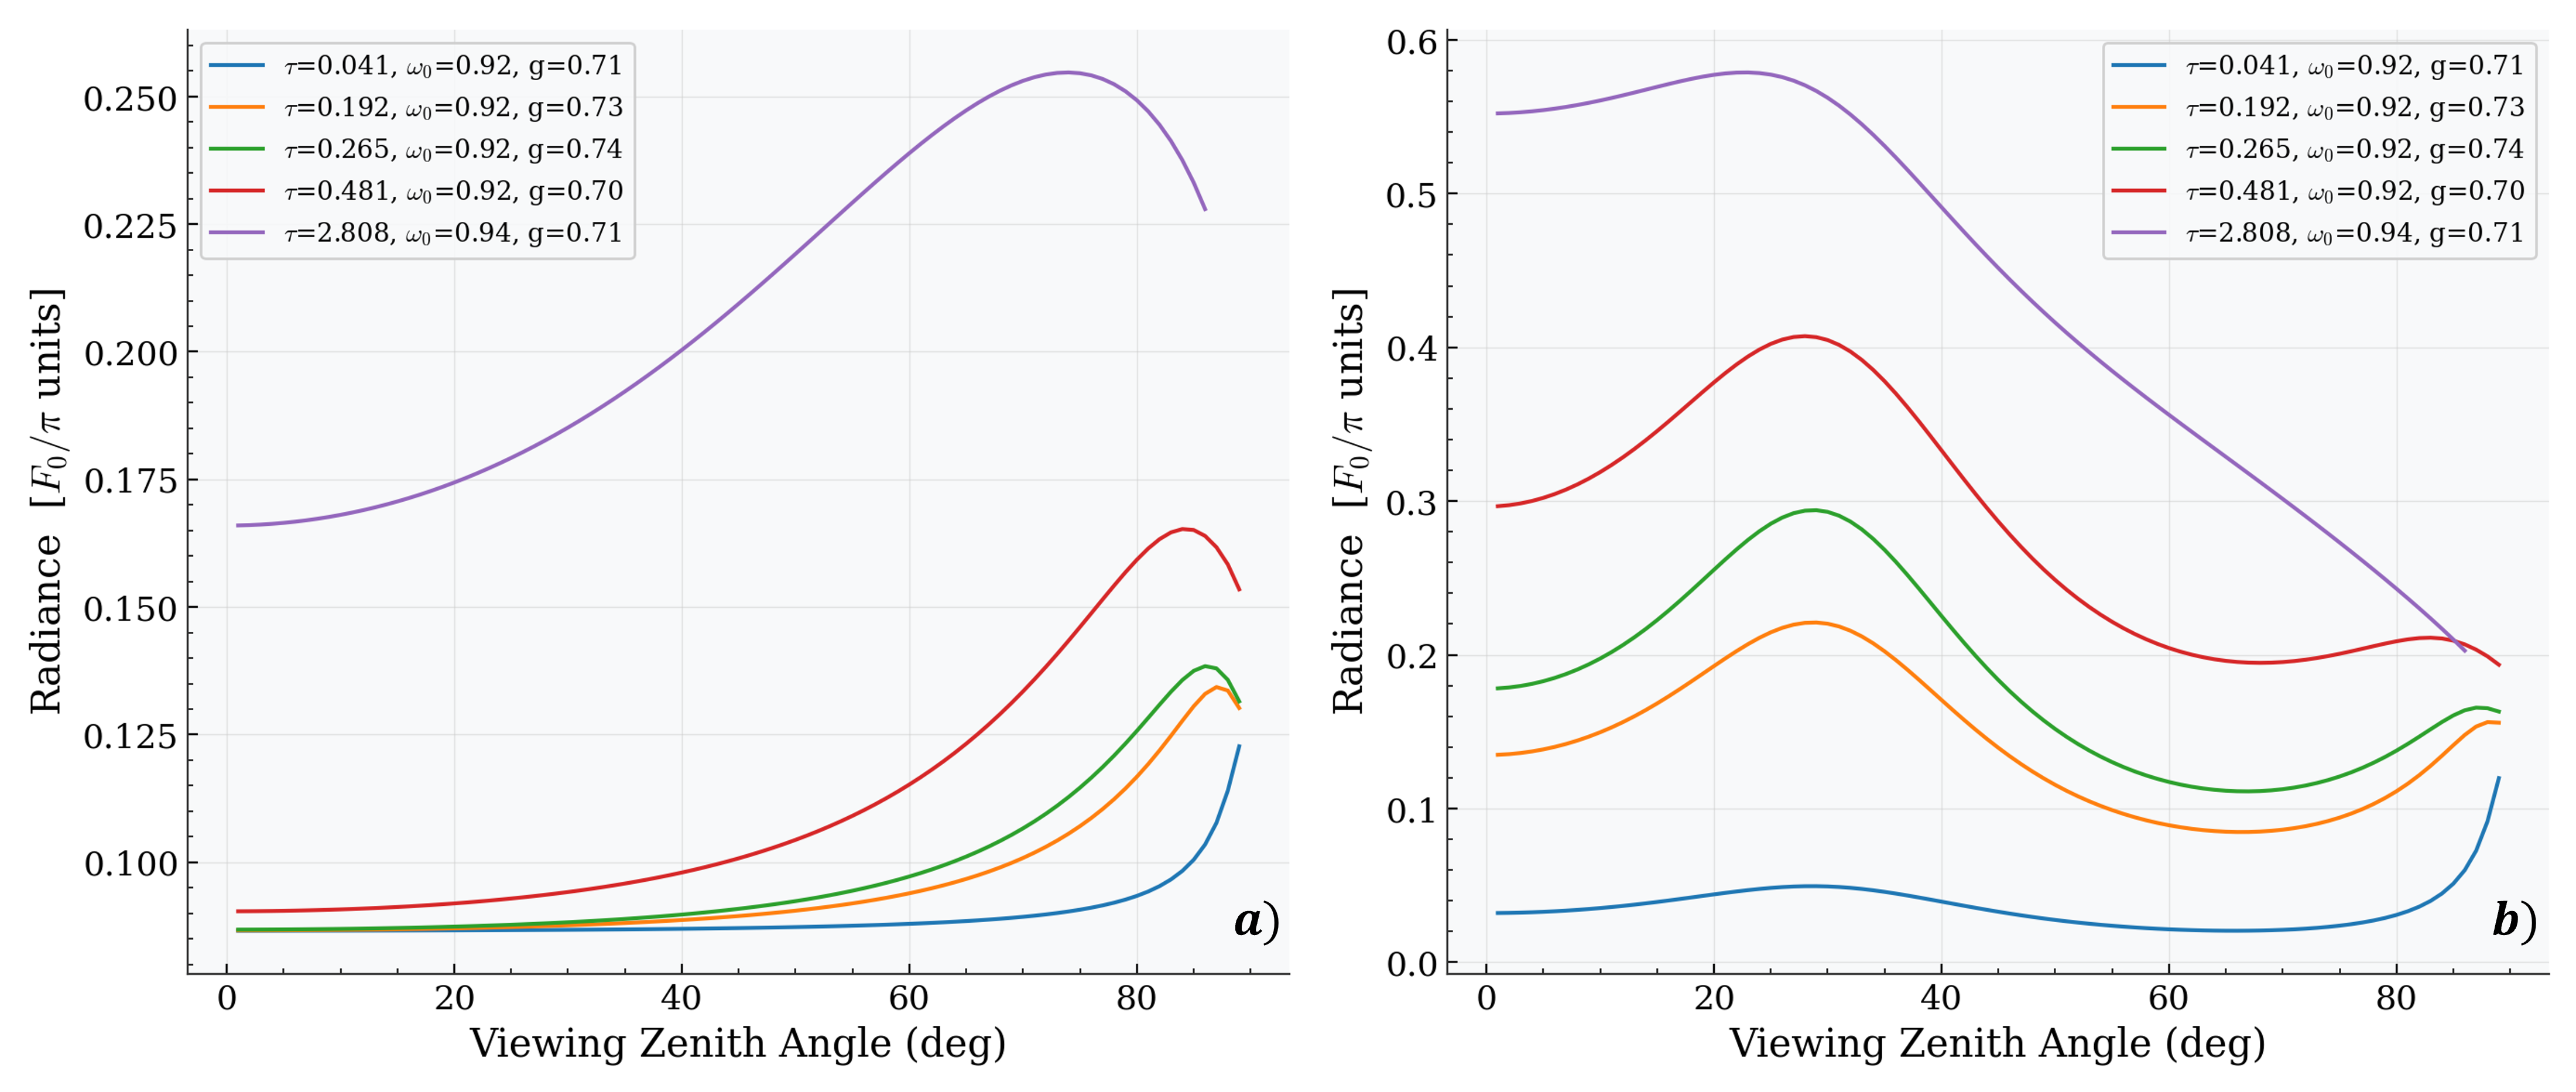
\includegraphics[width=\textwidth]{Images_final_report/Level3_AERONET_radiance_field_N36_theta030.png}
	\caption{DISORT-modelled radiance fields using AERONET-measured aerosol parameters for five selected days at the Bondville site.
	$N=36$ streams, $\theta_0=30^{\circ}$.
	(a)~TOA upwelling radiance. (b)~BOA downwelling radiance.
	Each curve is labelled with the corresponding AERONET values ($\tau$, $\omega_0$, $g$).}
	\label{fig:level3_radiance}
\end{figure}

\begin{figure}[H]
	\centering
	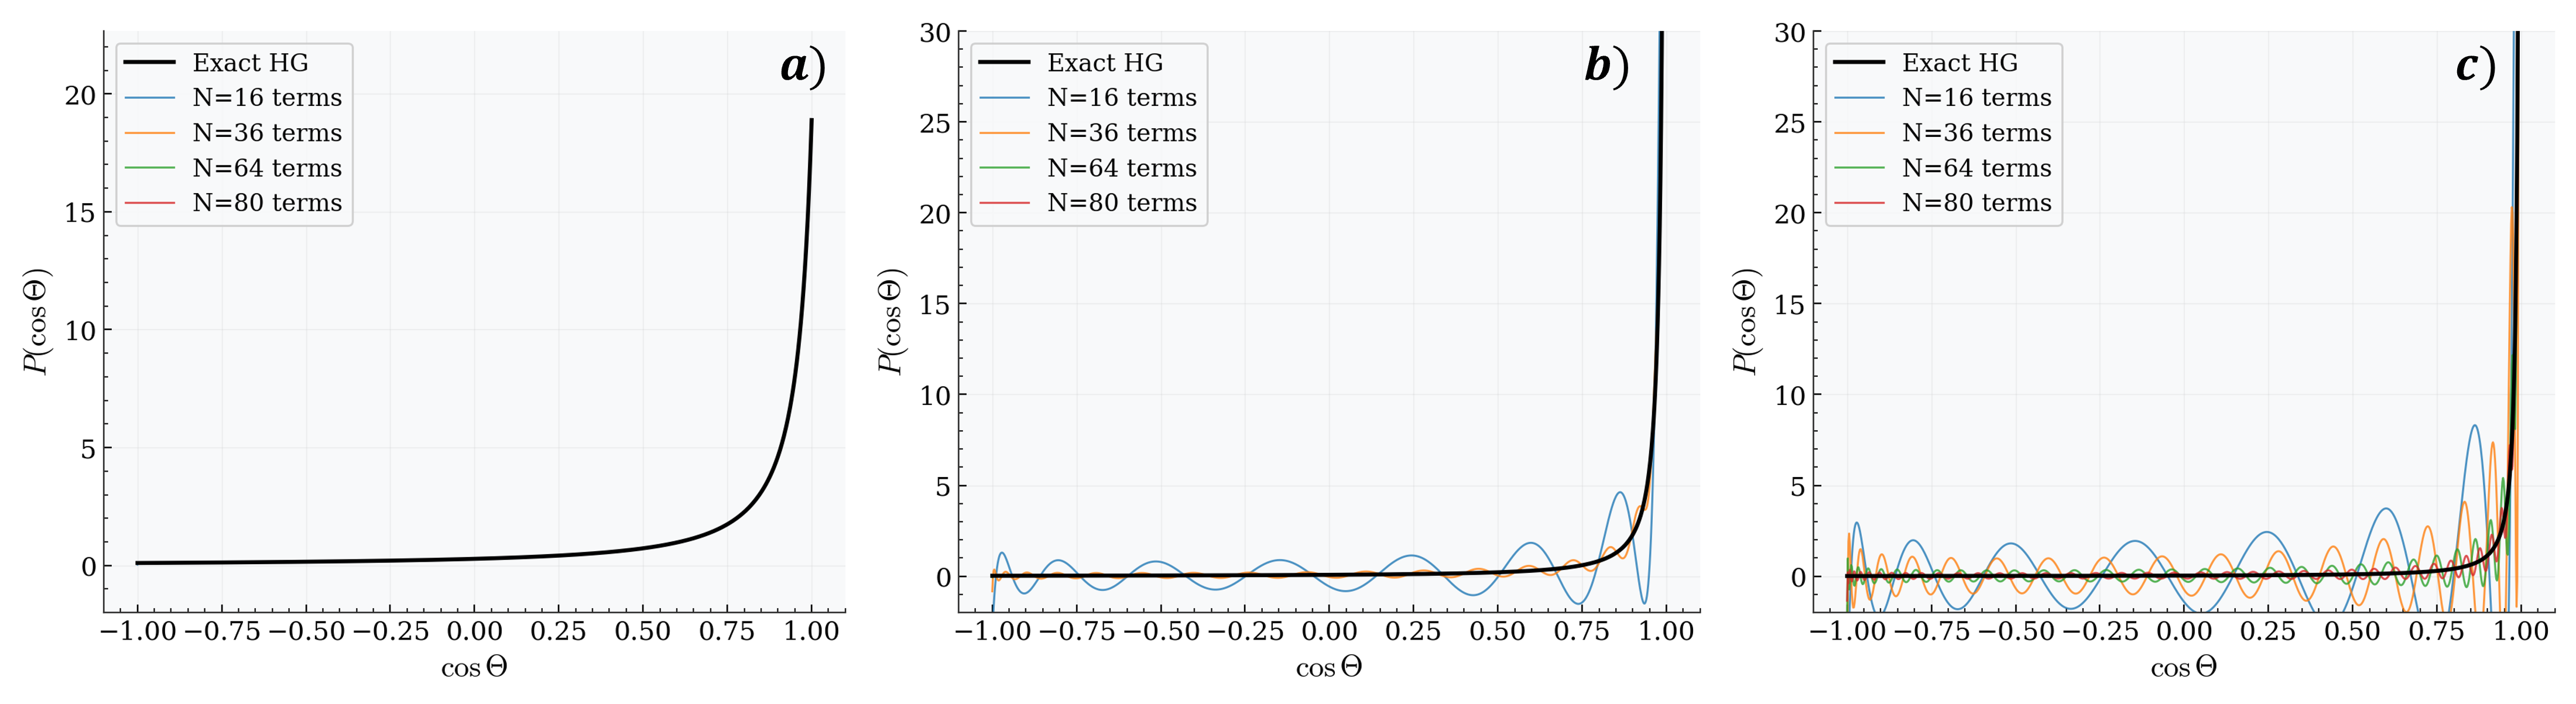
\includegraphics[width=\textwidth]{Images_final_report/diag_legendre_truncation_g07_g09_g095.png}
	\caption{Legendre polynomial expansion of the Henyey--Greenstein phase function truncated at $N = 16$, 36, 64, and 80 terms (coloured lines), compared with the exact analytical expression (black line).
	(a)~$g = 0.7$: all truncation orders converge to the exact result.
	(b)~$g = 0.9$: $N = 16$ shows Gibbs oscillations; $N \geq 36$ is adequate.
	(c)~$g = 0.95$: even $N = 80$ exhibits residual oscillations near the forward peak, demonstrating the need for delta-M scaling at high asymmetry parameters.}
	\label{fig:legendre_truncation}
\end{figure}

\begin{figure}[H]
	\centering
	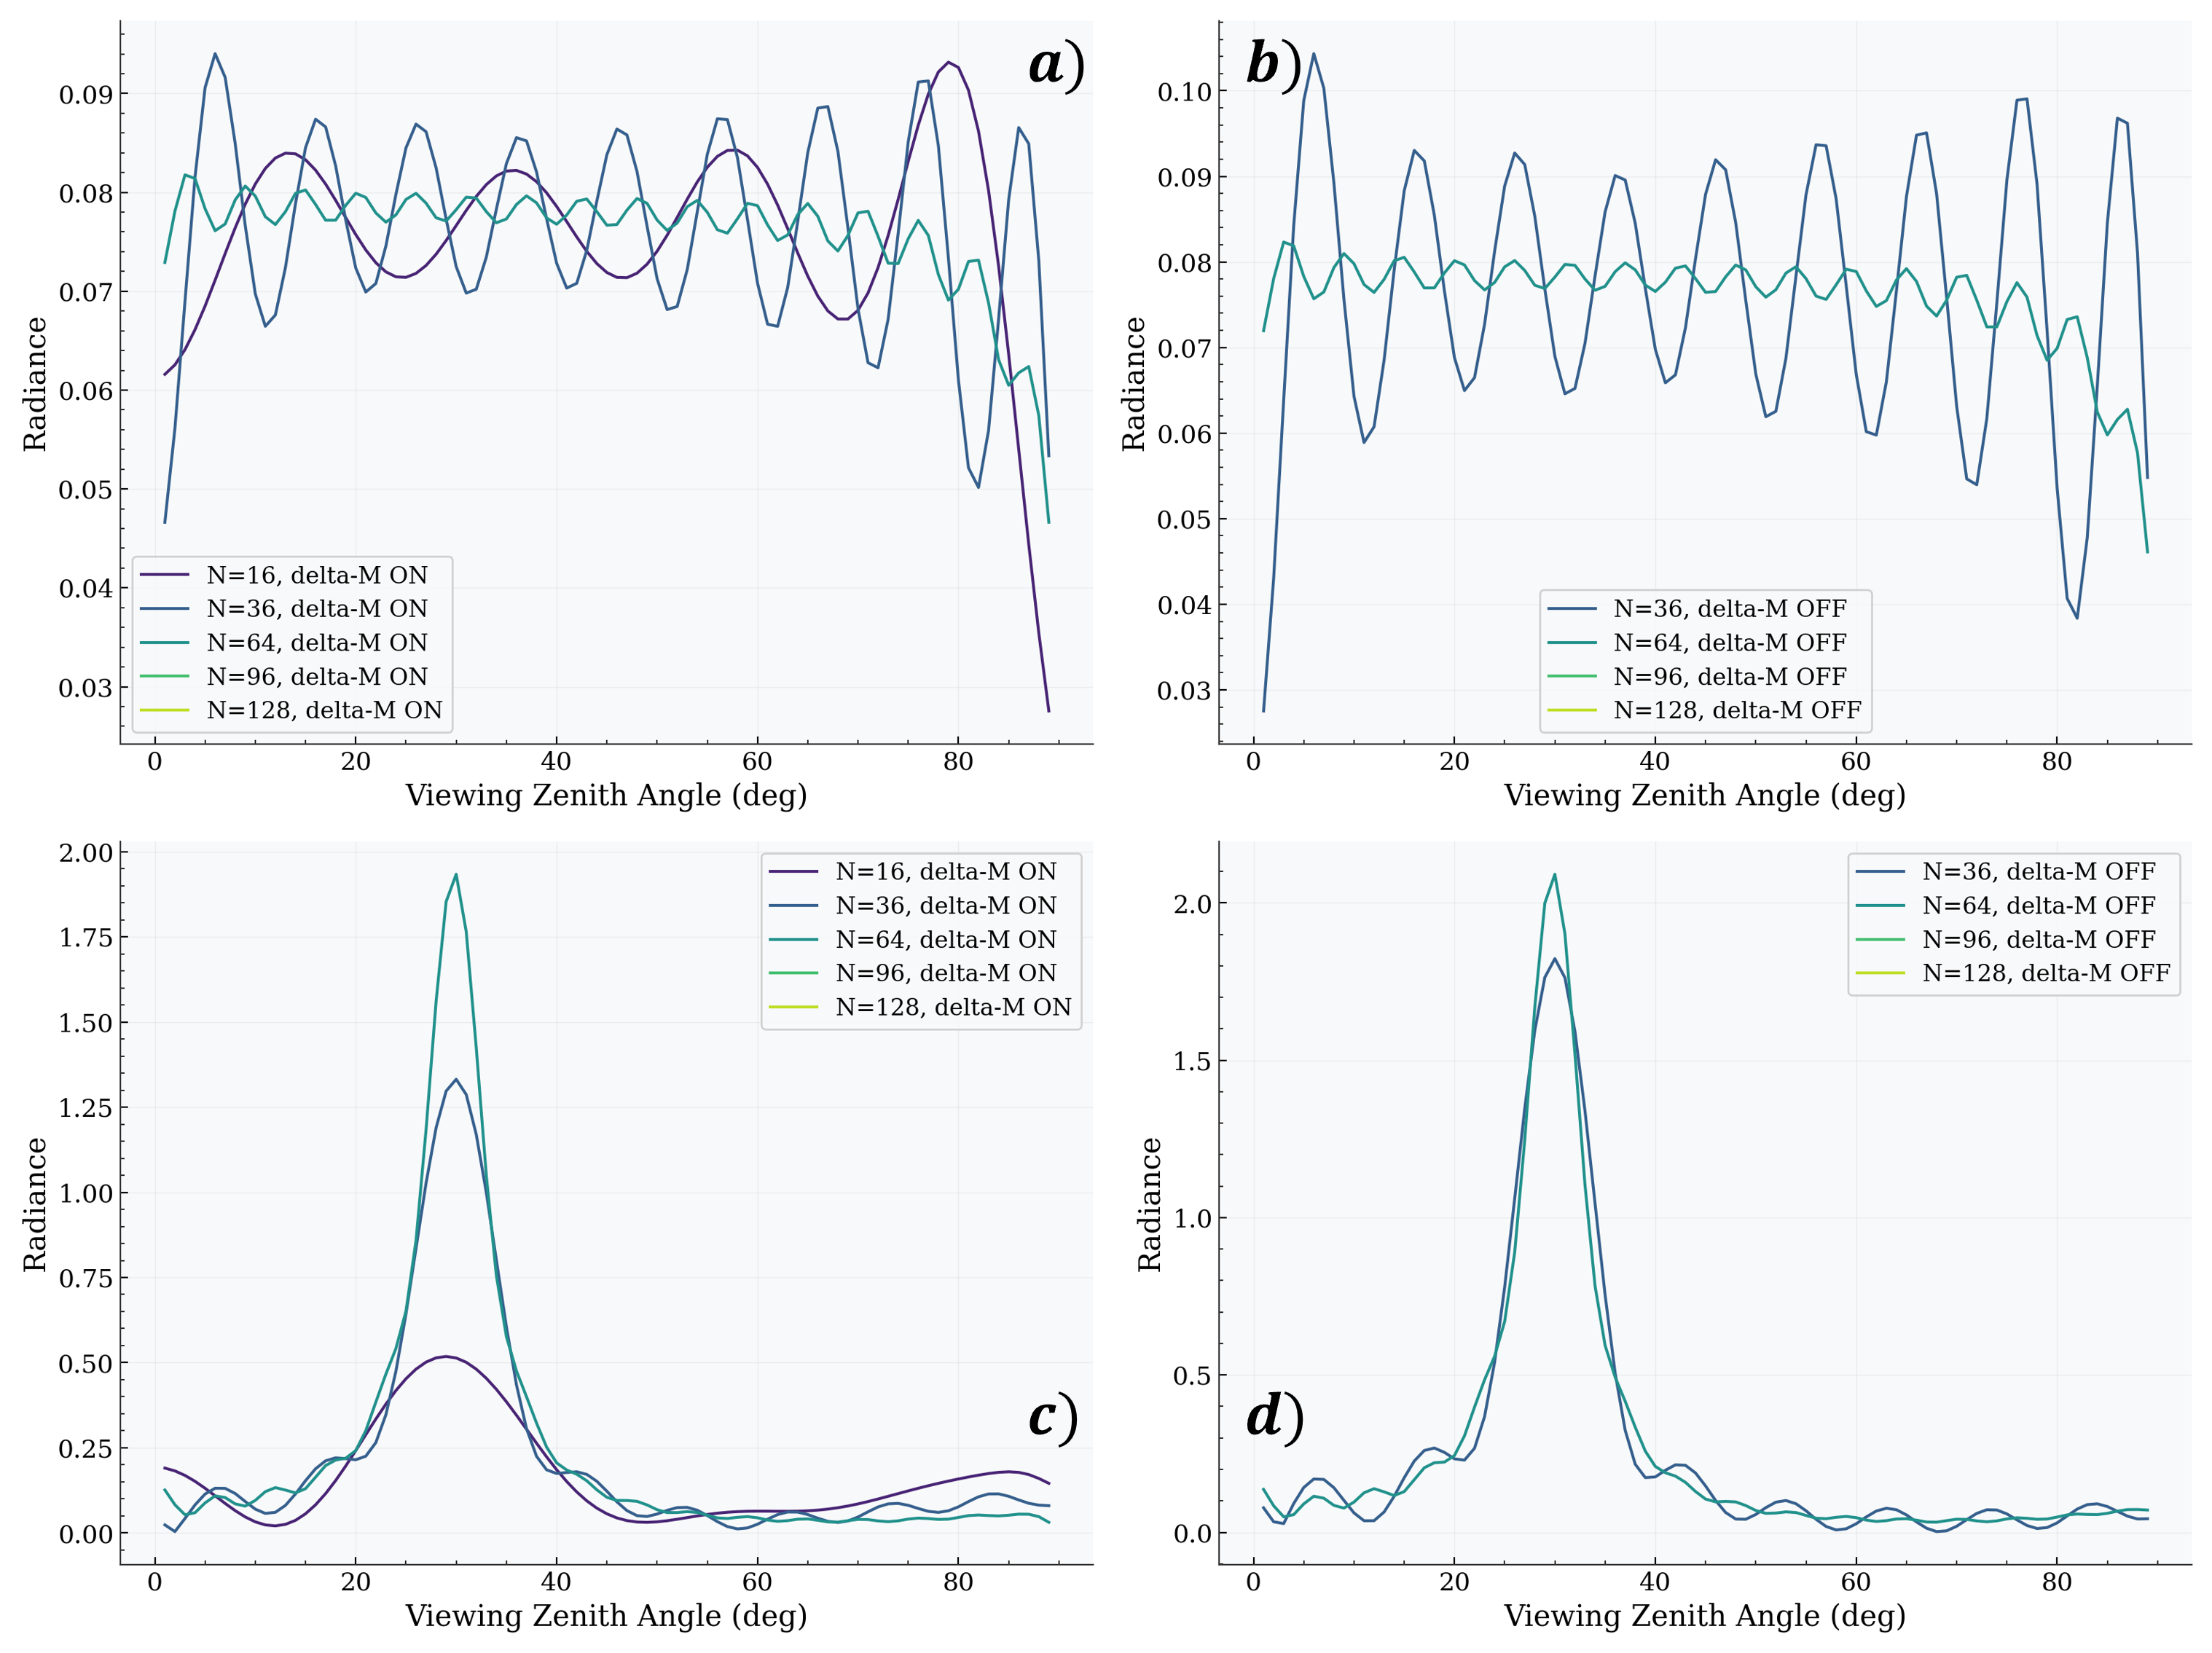
\includegraphics[width=\textwidth]{Images_final_report/diag_g095_streams_AOD_05_SSA_09_g095_theta030.png}
	\caption{Stream convergence study for a strongly forward-scattering phase function ($g=0.95$, $\tau=0.5$, $\omega_0=0.9$, $A_s=0.1$, $\theta_0=30^{\circ}$).
		Left column: delta-M scaling ON; right column: delta-M scaling OFF.
		(a)~TOA upwelling with delta-M ON.
		(b)~TOA upwelling with delta-M OFF.
		(c)~BOA downwelling with delta-M ON.
		(d)~BOA downwelling with delta-M OFF.}
	\label{fig:g095_streams}
\end{figure}
\end{document}
